% !TEX root = ../sethomas_thesis_main.tex
\section{Validation using a Case Study: A Multi-Output SMA Mandrel}\label{sec:smacm-mandrel}
\subsection{Motivation and Background}
As previously stated, Shape Memory Alloys exhibit a relatively high volumetric work density. Thus, they are an ideal candidate in created lightweight actuators for applications where reducing the total weight of the system drastically improves the efficiency such as drone deliveries. Here, any reduced weight increases the total flight time of the drone and thus, makes it the ideal use case of lightweight SMA actuators.
In the context of drone deliveries, grippers generally consist of an actuator such as a motor and kinematic stage that converts the motion of the actuator into a gripping motion. In certain scenarios, the required gripping motion can be complex consisting of multiple outputs and radial movements such as gripper implemented in \todocite (iris gripper).
In this case study, the goal is to apply the design methodology presented in this chapter to fabricate a drone-ready gripper with an advanced gripping mechanism. Using compliant mechanisms generated by topology optimization, an advanced kinematic stage can be designed to convert the motion of the SMA actuator into a multi-output gripping motion. Based on the design approach, the multi-output SMA gripper is sized and fabricated so as to validate the methodology.
\subsection{Working Principle of the Gripper}
The working principle of the proposed SMA gripper is based on the traditional SMA actuator presented in \cref{chap:sma-actuator-design} adapted by the design methodology described in \cref{chap:design-methodology}. Here, the gripper consists of a simple SMA coil that acts as the active element and an accompanying compliant structure that behaves as the kinematic stage and as the biasing element.

The active SMA coil is prestretched by the biasing element at low temperature and contracts when heated above its transition temperature. The biasing element, which also acts as a conversion mechanism to transform the linear actuation of the SMA coil into a gripper movement, exhibits an inherent stiffness due to the fact that it composed of flexure-based hinges. As the SMA cools down, a spring force acts on the coil due to the stiffness of the compliant mechanism. When heating the SMA, the contraction of the coil deforms the compliant biasing element creating the desired gripping motion at the output. By controlling the temperature of the SMA coil, the entire system can be made to grip and release objects.

In this application, the SMA coil is heating using Joule's heating by applying a constant voltage across it. This simple solution makes use of the internal resistance of the SMA coil to exploit the Joule's losses when passing a current through it to raise the temperature of the material. The coil, here, is cooled using passive cooling by simple convection with the surrounding air. This standard solution allows for a simple control system that does not require any external heating system which would add weight to the system. Furthermore, an H-bridge is used to supply the current and control the heating of the SMA coil. Finally, as precise control of the system is required, a hall-effect sensor or any other low profile position sensor can be used to detect the state of the gripper.

\begin{figure}[hbt!] % t for top of the page, H could be put to impose the position of the float
  \centering
  \resizebox{0.6\textwidth}{!}{%% Creator: Matplotlib, PGF backend
%%
%% To include the figure in your LaTeX document, write
%%   \input{<filename>.pgf}
%%
%% Make sure the required packages are loaded in your preamble
%%   \usepackage{pgf}
%%
%% Figures using additional raster images can only be included by \input if
%% they are in the same directory as the main LaTeX file. For loading figures
%% from other directories you can use the `import` package
%%   \usepackage{import}
%% and then include the figures with
%%   \import{<path to file>}{<filename>.pgf}
%%
%% Matplotlib used the following preamble
%%
\begingroup%
\makeatletter%
\begin{pgfpicture}%
\pgfpathrectangle{\pgfpointorigin}{\pgfqpoint{5.628569in}{4.423493in}}%
\pgfusepath{use as bounding box, clip}%
\begin{pgfscope}%
\pgfsetbuttcap%
\pgfsetmiterjoin%
\pgfsetlinewidth{0.000000pt}%
\definecolor{currentstroke}{rgb}{0.000000,0.000000,0.000000}%
\pgfsetstrokecolor{currentstroke}%
\pgfsetstrokeopacity{0.000000}%
\pgfsetdash{}{0pt}%
\pgfpathmoveto{\pgfqpoint{0.000000in}{0.000000in}}%
\pgfpathlineto{\pgfqpoint{5.628569in}{0.000000in}}%
\pgfpathlineto{\pgfqpoint{5.628569in}{4.423493in}}%
\pgfpathlineto{\pgfqpoint{0.000000in}{4.423493in}}%
\pgfpathclose%
\pgfusepath{}%
\end{pgfscope}%
\begin{pgfscope}%
\pgfsetbuttcap%
\pgfsetmiterjoin%
\pgfsetlinewidth{0.000000pt}%
\definecolor{currentstroke}{rgb}{0.000000,0.000000,0.000000}%
\pgfsetstrokecolor{currentstroke}%
\pgfsetstrokeopacity{0.000000}%
\pgfsetdash{}{0pt}%
\pgfpathmoveto{\pgfqpoint{0.437333in}{0.627493in}}%
\pgfpathlineto{\pgfqpoint{5.397333in}{0.627493in}}%
\pgfpathlineto{\pgfqpoint{5.397333in}{4.323493in}}%
\pgfpathlineto{\pgfqpoint{0.437333in}{4.323493in}}%
\pgfpathclose%
\pgfusepath{}%
\end{pgfscope}%
\begin{pgfscope}%
\pgfsetbuttcap%
\pgfsetmiterjoin%
\definecolor{currentfill}{rgb}{0.000000,0.000000,0.000000}%
\pgfsetfillcolor{currentfill}%
\pgfsetlinewidth{1.003750pt}%
\definecolor{currentstroke}{rgb}{0.000000,0.000000,0.000000}%
\pgfsetstrokecolor{currentstroke}%
\pgfsetdash{}{0pt}%
\pgfpathmoveto{\pgfqpoint{5.397333in}{0.627493in}}%
\pgfpathlineto{\pgfqpoint{5.273333in}{0.581293in}}%
\pgfpathlineto{\pgfqpoint{5.310533in}{0.627401in}}%
\pgfpathlineto{\pgfqpoint{0.437333in}{0.627401in}}%
\pgfpathlineto{\pgfqpoint{0.437333in}{0.627584in}}%
\pgfpathlineto{\pgfqpoint{5.310533in}{0.627584in}}%
\pgfpathlineto{\pgfqpoint{5.273333in}{0.673693in}}%
\pgfpathclose%
\pgfusepath{stroke,fill}%
\end{pgfscope}%
\begin{pgfscope}%
\pgfsetbuttcap%
\pgfsetmiterjoin%
\definecolor{currentfill}{rgb}{0.000000,0.000000,0.000000}%
\pgfsetfillcolor{currentfill}%
\pgfsetlinewidth{1.003750pt}%
\definecolor{currentstroke}{rgb}{0.000000,0.000000,0.000000}%
\pgfsetstrokecolor{currentstroke}%
\pgfsetdash{}{0pt}%
\pgfpathmoveto{\pgfqpoint{0.437333in}{4.323493in}}%
\pgfpathlineto{\pgfqpoint{0.483533in}{4.199493in}}%
\pgfpathlineto{\pgfqpoint{0.437625in}{4.236693in}}%
\pgfpathlineto{\pgfqpoint{0.437625in}{0.627493in}}%
\pgfpathlineto{\pgfqpoint{0.437041in}{0.627493in}}%
\pgfpathlineto{\pgfqpoint{0.437041in}{4.236693in}}%
\pgfpathlineto{\pgfqpoint{0.391133in}{4.199493in}}%
\pgfpathclose%
\pgfusepath{stroke,fill}%
\end{pgfscope}%
\begin{pgfscope}%
\pgfsetbuttcap%
\pgfsetroundjoin%
\definecolor{currentfill}{rgb}{0.000000,0.000000,0.000000}%
\pgfsetfillcolor{currentfill}%
\pgfsetlinewidth{0.803000pt}%
\definecolor{currentstroke}{rgb}{0.000000,0.000000,0.000000}%
\pgfsetstrokecolor{currentstroke}%
\pgfsetdash{}{0pt}%
\pgfsys@defobject{currentmarker}{\pgfqpoint{0.000000in}{-0.048611in}}{\pgfqpoint{0.000000in}{0.000000in}}{%
\pgfpathmoveto{\pgfqpoint{0.000000in}{0.000000in}}%
\pgfpathlineto{\pgfqpoint{0.000000in}{-0.048611in}}%
\pgfusepath{stroke,fill}%
}%
\begin{pgfscope}%
\pgfsys@transformshift{0.437333in}{0.627493in}%
\pgfsys@useobject{currentmarker}{}%
\end{pgfscope}%
\end{pgfscope}%
\begin{pgfscope}%
\definecolor{textcolor}{rgb}{0.000000,0.000000,0.000000}%
\pgfsetstrokecolor{textcolor}%
\pgfsetfillcolor{textcolor}%
\pgftext[x=0.437333in,y=0.530271in,,top]{\color{textcolor}\rmfamily\fontsize{16.000000}{19.200000}\selectfont 0}%
\end{pgfscope}%
\begin{pgfscope}%
\pgfsetbuttcap%
\pgfsetroundjoin%
\definecolor{currentfill}{rgb}{0.000000,0.000000,0.000000}%
\pgfsetfillcolor{currentfill}%
\pgfsetlinewidth{0.803000pt}%
\definecolor{currentstroke}{rgb}{0.000000,0.000000,0.000000}%
\pgfsetstrokecolor{currentstroke}%
\pgfsetdash{}{0pt}%
\pgfsys@defobject{currentmarker}{\pgfqpoint{0.000000in}{-0.048611in}}{\pgfqpoint{0.000000in}{0.000000in}}{%
\pgfpathmoveto{\pgfqpoint{0.000000in}{0.000000in}}%
\pgfpathlineto{\pgfqpoint{0.000000in}{-0.048611in}}%
\pgfusepath{stroke,fill}%
}%
\begin{pgfscope}%
\pgfsys@transformshift{3.854481in}{0.627493in}%
\pgfsys@useobject{currentmarker}{}%
\end{pgfscope}%
\end{pgfscope}%
\begin{pgfscope}%
\definecolor{textcolor}{rgb}{0.000000,0.000000,0.000000}%
\pgfsetstrokecolor{textcolor}%
\pgfsetfillcolor{textcolor}%
\pgftext[x=3.854481in,y=0.530271in,,top]{\color{textcolor}\rmfamily\fontsize{16.000000}{19.200000}\selectfont \(\displaystyle x_1\)}%
\end{pgfscope}%
\begin{pgfscope}%
\pgfsetbuttcap%
\pgfsetroundjoin%
\definecolor{currentfill}{rgb}{0.000000,0.000000,0.000000}%
\pgfsetfillcolor{currentfill}%
\pgfsetlinewidth{0.803000pt}%
\definecolor{currentstroke}{rgb}{0.000000,0.000000,0.000000}%
\pgfsetstrokecolor{currentstroke}%
\pgfsetdash{}{0pt}%
\pgfsys@defobject{currentmarker}{\pgfqpoint{0.000000in}{-0.048611in}}{\pgfqpoint{0.000000in}{0.000000in}}{%
\pgfpathmoveto{\pgfqpoint{0.000000in}{0.000000in}}%
\pgfpathlineto{\pgfqpoint{0.000000in}{-0.048611in}}%
\pgfusepath{stroke,fill}%
}%
\begin{pgfscope}%
\pgfsys@transformshift{2.771451in}{0.627493in}%
\pgfsys@useobject{currentmarker}{}%
\end{pgfscope}%
\end{pgfscope}%
\begin{pgfscope}%
\definecolor{textcolor}{rgb}{0.000000,0.000000,0.000000}%
\pgfsetstrokecolor{textcolor}%
\pgfsetfillcolor{textcolor}%
\pgftext[x=2.771451in,y=0.530271in,,top]{\color{textcolor}\rmfamily\fontsize{16.000000}{19.200000}\selectfont \(\displaystyle x\)\(\displaystyle _{\textrm{Obj}}\)}%
\end{pgfscope}%
\begin{pgfscope}%
\pgfsetbuttcap%
\pgfsetroundjoin%
\definecolor{currentfill}{rgb}{0.000000,0.000000,0.000000}%
\pgfsetfillcolor{currentfill}%
\pgfsetlinewidth{0.803000pt}%
\definecolor{currentstroke}{rgb}{0.000000,0.000000,0.000000}%
\pgfsetstrokecolor{currentstroke}%
\pgfsetdash{}{0pt}%
\pgfsys@defobject{currentmarker}{\pgfqpoint{0.000000in}{-0.048611in}}{\pgfqpoint{0.000000in}{0.000000in}}{%
\pgfpathmoveto{\pgfqpoint{0.000000in}{0.000000in}}%
\pgfpathlineto{\pgfqpoint{0.000000in}{-0.048611in}}%
\pgfusepath{stroke,fill}%
}%
\begin{pgfscope}%
\pgfsys@transformshift{1.415328in}{0.627493in}%
\pgfsys@useobject{currentmarker}{}%
\end{pgfscope}%
\end{pgfscope}%
\begin{pgfscope}%
\definecolor{textcolor}{rgb}{0.000000,0.000000,0.000000}%
\pgfsetstrokecolor{textcolor}%
\pgfsetfillcolor{textcolor}%
\pgftext[x=1.415328in,y=0.530271in,,top]{\color{textcolor}\rmfamily\fontsize{16.000000}{19.200000}\selectfont \(\displaystyle x_2\)}%
\end{pgfscope}%
\begin{pgfscope}%
\pgfsetbuttcap%
\pgfsetroundjoin%
\definecolor{currentfill}{rgb}{0.000000,0.000000,0.000000}%
\pgfsetfillcolor{currentfill}%
\pgfsetlinewidth{0.803000pt}%
\definecolor{currentstroke}{rgb}{0.000000,0.000000,0.000000}%
\pgfsetstrokecolor{currentstroke}%
\pgfsetdash{}{0pt}%
\pgfsys@defobject{currentmarker}{\pgfqpoint{0.000000in}{-0.048611in}}{\pgfqpoint{0.000000in}{0.000000in}}{%
\pgfpathmoveto{\pgfqpoint{0.000000in}{0.000000in}}%
\pgfpathlineto{\pgfqpoint{0.000000in}{-0.048611in}}%
\pgfusepath{stroke,fill}%
}%
\begin{pgfscope}%
\pgfsys@transformshift{5.105568in}{0.627493in}%
\pgfsys@useobject{currentmarker}{}%
\end{pgfscope}%
\end{pgfscope}%
\begin{pgfscope}%
\definecolor{textcolor}{rgb}{0.000000,0.000000,0.000000}%
\pgfsetstrokecolor{textcolor}%
\pgfsetfillcolor{textcolor}%
\pgftext[x=5.105568in,y=0.530271in,,top]{\color{textcolor}\rmfamily\fontsize{16.000000}{19.200000}\selectfont \(\displaystyle x_{\textrm{off}}\)}%
\end{pgfscope}%
\begin{pgfscope}%
\definecolor{textcolor}{rgb}{0.000000,0.000000,0.000000}%
\pgfsetstrokecolor{textcolor}%
\pgfsetfillcolor{textcolor}%
\pgftext[x=5.149333in,y=0.313333in,,top]{\color{textcolor}\rmfamily\fontsize{18.000000}{21.600000}\bfseries\selectfont Stroke}%
\end{pgfscope}%
\begin{pgfscope}%
\pgfsetbuttcap%
\pgfsetroundjoin%
\definecolor{currentfill}{rgb}{0.000000,0.000000,0.000000}%
\pgfsetfillcolor{currentfill}%
\pgfsetlinewidth{0.803000pt}%
\definecolor{currentstroke}{rgb}{0.000000,0.000000,0.000000}%
\pgfsetstrokecolor{currentstroke}%
\pgfsetdash{}{0pt}%
\pgfsys@defobject{currentmarker}{\pgfqpoint{-0.048611in}{0.000000in}}{\pgfqpoint{0.000000in}{0.000000in}}{%
\pgfpathmoveto{\pgfqpoint{0.000000in}{0.000000in}}%
\pgfpathlineto{\pgfqpoint{-0.048611in}{0.000000in}}%
\pgfusepath{stroke,fill}%
}%
\begin{pgfscope}%
\pgfsys@transformshift{0.437333in}{0.627493in}%
\pgfsys@useobject{currentmarker}{}%
\end{pgfscope}%
\end{pgfscope}%
\begin{pgfscope}%
\definecolor{textcolor}{rgb}{0.000000,0.000000,0.000000}%
\pgfsetstrokecolor{textcolor}%
\pgfsetfillcolor{textcolor}%
\pgftext[x=0.293429in,y=0.572459in,left,base,rotate=90.000000]{\color{textcolor}\rmfamily\fontsize{16.000000}{19.200000}\selectfont 0}%
\end{pgfscope}%
\begin{pgfscope}%
\pgfsetbuttcap%
\pgfsetroundjoin%
\definecolor{currentfill}{rgb}{0.000000,0.000000,0.000000}%
\pgfsetfillcolor{currentfill}%
\pgfsetlinewidth{0.803000pt}%
\definecolor{currentstroke}{rgb}{0.000000,0.000000,0.000000}%
\pgfsetstrokecolor{currentstroke}%
\pgfsetdash{}{0pt}%
\pgfsys@defobject{currentmarker}{\pgfqpoint{-0.048611in}{0.000000in}}{\pgfqpoint{0.000000in}{0.000000in}}{%
\pgfpathmoveto{\pgfqpoint{0.000000in}{0.000000in}}%
\pgfpathlineto{\pgfqpoint{-0.048611in}{0.000000in}}%
\pgfusepath{stroke,fill}%
}%
\begin{pgfscope}%
\pgfsys@transformshift{0.437333in}{2.823136in}%
\pgfsys@useobject{currentmarker}{}%
\end{pgfscope}%
\end{pgfscope}%
\begin{pgfscope}%
\definecolor{textcolor}{rgb}{0.000000,0.000000,0.000000}%
\pgfsetstrokecolor{textcolor}%
\pgfsetfillcolor{textcolor}%
\pgftext[x=0.293429in,y=2.705581in,left,base,rotate=90.000000]{\color{textcolor}\rmfamily\fontsize{16.000000}{19.200000}\selectfont \(\displaystyle F_{3}\)}%
\end{pgfscope}%
\begin{pgfscope}%
\definecolor{textcolor}{rgb}{0.000000,0.000000,0.000000}%
\pgfsetstrokecolor{textcolor}%
\pgfsetfillcolor{textcolor}%
\pgftext[x=0.313333in,y=3.953893in,,bottom,rotate=90.000000]{\color{textcolor}\rmfamily\fontsize{18.000000}{21.600000}\bfseries\selectfont Force}%
\end{pgfscope}%
\begin{pgfscope}%
\pgfpathrectangle{\pgfqpoint{0.437333in}{0.627493in}}{\pgfqpoint{4.960000in}{3.696000in}}%
\pgfusepath{clip}%
\pgfsetrectcap%
\pgfsetroundjoin%
\pgfsetlinewidth{2.007500pt}%
\definecolor{currentstroke}{rgb}{0.000000,0.447059,0.741176}%
\pgfsetstrokecolor{currentstroke}%
\pgfsetdash{}{0pt}%
\pgfpathmoveto{\pgfqpoint{0.437333in}{0.627493in}}%
\pgfpathlineto{\pgfqpoint{0.484487in}{0.634886in}}%
\pgfpathlineto{\pgfqpoint{0.531641in}{0.642278in}}%
\pgfpathlineto{\pgfqpoint{0.578795in}{0.649671in}}%
\pgfpathlineto{\pgfqpoint{0.625948in}{0.657064in}}%
\pgfpathlineto{\pgfqpoint{0.673102in}{0.664457in}}%
\pgfpathlineto{\pgfqpoint{0.720256in}{0.671849in}}%
\pgfpathlineto{\pgfqpoint{0.767410in}{0.679242in}}%
\pgfpathlineto{\pgfqpoint{0.814564in}{0.686635in}}%
\pgfpathlineto{\pgfqpoint{0.861718in}{0.694028in}}%
\pgfpathlineto{\pgfqpoint{0.908872in}{0.701420in}}%
\pgfpathlineto{\pgfqpoint{0.956026in}{0.708813in}}%
\pgfpathlineto{\pgfqpoint{1.003180in}{0.716206in}}%
\pgfpathlineto{\pgfqpoint{1.050334in}{0.723599in}}%
\pgfpathlineto{\pgfqpoint{1.097487in}{0.730991in}}%
\pgfpathlineto{\pgfqpoint{1.144641in}{0.738384in}}%
\pgfpathlineto{\pgfqpoint{1.191795in}{0.745777in}}%
\pgfpathlineto{\pgfqpoint{1.238949in}{0.753169in}}%
\pgfpathlineto{\pgfqpoint{1.286103in}{0.760562in}}%
\pgfpathlineto{\pgfqpoint{1.333257in}{0.767955in}}%
\pgfpathlineto{\pgfqpoint{1.380411in}{0.775348in}}%
\pgfpathlineto{\pgfqpoint{1.427565in}{0.782740in}}%
\pgfpathlineto{\pgfqpoint{1.474719in}{0.790133in}}%
\pgfpathlineto{\pgfqpoint{1.521872in}{0.797526in}}%
\pgfpathlineto{\pgfqpoint{1.569026in}{0.804919in}}%
\pgfpathlineto{\pgfqpoint{1.616180in}{0.812311in}}%
\pgfpathlineto{\pgfqpoint{1.663334in}{0.819704in}}%
\pgfpathlineto{\pgfqpoint{1.710488in}{0.827097in}}%
\pgfpathlineto{\pgfqpoint{1.757642in}{0.834490in}}%
\pgfpathlineto{\pgfqpoint{1.804796in}{0.841882in}}%
\pgfpathlineto{\pgfqpoint{1.851950in}{0.849275in}}%
\pgfpathlineto{\pgfqpoint{1.899104in}{0.856668in}}%
\pgfpathlineto{\pgfqpoint{1.946257in}{0.864061in}}%
\pgfpathlineto{\pgfqpoint{1.993411in}{0.871453in}}%
\pgfpathlineto{\pgfqpoint{2.040565in}{0.878846in}}%
\pgfpathlineto{\pgfqpoint{2.087719in}{0.886239in}}%
\pgfpathlineto{\pgfqpoint{2.134873in}{0.893632in}}%
\pgfpathlineto{\pgfqpoint{2.182027in}{0.901024in}}%
\pgfpathlineto{\pgfqpoint{2.229181in}{0.908417in}}%
\pgfpathlineto{\pgfqpoint{2.276335in}{0.915810in}}%
\pgfpathlineto{\pgfqpoint{2.323489in}{0.923202in}}%
\pgfpathlineto{\pgfqpoint{2.370642in}{0.930595in}}%
\pgfpathlineto{\pgfqpoint{2.417796in}{0.937988in}}%
\pgfpathlineto{\pgfqpoint{2.464950in}{0.945381in}}%
\pgfpathlineto{\pgfqpoint{2.512104in}{0.952773in}}%
\pgfpathlineto{\pgfqpoint{2.559258in}{0.960166in}}%
\pgfpathlineto{\pgfqpoint{2.606412in}{0.967559in}}%
\pgfpathlineto{\pgfqpoint{2.653566in}{0.974952in}}%
\pgfpathlineto{\pgfqpoint{2.700720in}{0.982344in}}%
\pgfpathlineto{\pgfqpoint{2.747874in}{0.989737in}}%
\pgfpathlineto{\pgfqpoint{2.795028in}{0.997130in}}%
\pgfpathlineto{\pgfqpoint{2.842181in}{1.004523in}}%
\pgfpathlineto{\pgfqpoint{2.889335in}{1.011915in}}%
\pgfpathlineto{\pgfqpoint{2.936489in}{1.019308in}}%
\pgfpathlineto{\pgfqpoint{2.983643in}{1.026701in}}%
\pgfpathlineto{\pgfqpoint{3.030797in}{1.034094in}}%
\pgfpathlineto{\pgfqpoint{3.077951in}{1.041486in}}%
\pgfpathlineto{\pgfqpoint{3.125105in}{1.048879in}}%
\pgfpathlineto{\pgfqpoint{3.172259in}{1.056272in}}%
\pgfpathlineto{\pgfqpoint{3.219413in}{1.063665in}}%
\pgfpathlineto{\pgfqpoint{3.266566in}{1.071057in}}%
\pgfpathlineto{\pgfqpoint{3.313720in}{1.078450in}}%
\pgfpathlineto{\pgfqpoint{3.360874in}{1.085843in}}%
\pgfpathlineto{\pgfqpoint{3.408028in}{1.093235in}}%
\pgfpathlineto{\pgfqpoint{3.455182in}{1.100628in}}%
\pgfpathlineto{\pgfqpoint{3.502336in}{1.108021in}}%
\pgfpathlineto{\pgfqpoint{3.549490in}{1.115414in}}%
\pgfpathlineto{\pgfqpoint{3.596644in}{1.122806in}}%
\pgfpathlineto{\pgfqpoint{3.643798in}{1.130199in}}%
\pgfpathlineto{\pgfqpoint{3.690951in}{1.137592in}}%
\pgfpathlineto{\pgfqpoint{3.738105in}{1.144985in}}%
\pgfpathlineto{\pgfqpoint{3.785259in}{1.152377in}}%
\pgfpathlineto{\pgfqpoint{3.832413in}{1.159770in}}%
\pgfpathlineto{\pgfqpoint{3.879567in}{1.167163in}}%
\pgfpathlineto{\pgfqpoint{3.926721in}{1.174556in}}%
\pgfpathlineto{\pgfqpoint{3.973875in}{1.181948in}}%
\pgfpathlineto{\pgfqpoint{4.021029in}{1.189341in}}%
\pgfpathlineto{\pgfqpoint{4.068183in}{1.196734in}}%
\pgfpathlineto{\pgfqpoint{4.115336in}{1.204127in}}%
\pgfpathlineto{\pgfqpoint{4.162490in}{1.211519in}}%
\pgfpathlineto{\pgfqpoint{4.209644in}{1.218912in}}%
\pgfpathlineto{\pgfqpoint{4.256798in}{1.226305in}}%
\pgfpathlineto{\pgfqpoint{4.303952in}{1.233698in}}%
\pgfpathlineto{\pgfqpoint{4.351106in}{1.241090in}}%
\pgfpathlineto{\pgfqpoint{4.398260in}{1.248483in}}%
\pgfpathlineto{\pgfqpoint{4.445414in}{1.255876in}}%
\pgfpathlineto{\pgfqpoint{4.492568in}{1.263268in}}%
\pgfpathlineto{\pgfqpoint{4.539722in}{1.270661in}}%
\pgfpathlineto{\pgfqpoint{4.586875in}{1.278054in}}%
\pgfpathlineto{\pgfqpoint{4.634029in}{1.285447in}}%
\pgfpathlineto{\pgfqpoint{4.681183in}{1.292839in}}%
\pgfpathlineto{\pgfqpoint{4.728337in}{1.300232in}}%
\pgfpathlineto{\pgfqpoint{4.775491in}{1.307625in}}%
\pgfpathlineto{\pgfqpoint{4.822645in}{1.315018in}}%
\pgfpathlineto{\pgfqpoint{4.869799in}{1.322410in}}%
\pgfpathlineto{\pgfqpoint{4.916953in}{1.329803in}}%
\pgfpathlineto{\pgfqpoint{4.964107in}{1.337196in}}%
\pgfpathlineto{\pgfqpoint{5.011260in}{1.344589in}}%
\pgfpathlineto{\pgfqpoint{5.058414in}{1.351981in}}%
\pgfpathlineto{\pgfqpoint{5.105568in}{1.359374in}}%
\pgfusepath{stroke}%
\end{pgfscope}%
\begin{pgfscope}%
\pgfpathrectangle{\pgfqpoint{0.437333in}{0.627493in}}{\pgfqpoint{4.960000in}{3.696000in}}%
\pgfusepath{clip}%
\pgfsetrectcap%
\pgfsetroundjoin%
\pgfsetlinewidth{2.007500pt}%
\definecolor{currentstroke}{rgb}{0.768627,0.000000,0.047059}%
\pgfsetstrokecolor{currentstroke}%
\pgfsetdash{}{0pt}%
\pgfpathmoveto{\pgfqpoint{0.437333in}{0.627493in}}%
\pgfpathlineto{\pgfqpoint{0.484487in}{0.671849in}}%
\pgfpathlineto{\pgfqpoint{0.531641in}{0.716206in}}%
\pgfpathlineto{\pgfqpoint{0.578795in}{0.760562in}}%
\pgfpathlineto{\pgfqpoint{0.625948in}{0.804919in}}%
\pgfpathlineto{\pgfqpoint{0.673102in}{0.849275in}}%
\pgfpathlineto{\pgfqpoint{0.720256in}{0.893632in}}%
\pgfpathlineto{\pgfqpoint{0.767410in}{0.937988in}}%
\pgfpathlineto{\pgfqpoint{0.814564in}{0.982344in}}%
\pgfpathlineto{\pgfqpoint{0.861718in}{1.026701in}}%
\pgfpathlineto{\pgfqpoint{0.908872in}{1.071057in}}%
\pgfpathlineto{\pgfqpoint{0.956026in}{1.115414in}}%
\pgfpathlineto{\pgfqpoint{1.003180in}{1.159770in}}%
\pgfpathlineto{\pgfqpoint{1.050334in}{1.204127in}}%
\pgfpathlineto{\pgfqpoint{1.097487in}{1.248483in}}%
\pgfpathlineto{\pgfqpoint{1.144641in}{1.292839in}}%
\pgfpathlineto{\pgfqpoint{1.191795in}{1.337196in}}%
\pgfpathlineto{\pgfqpoint{1.238949in}{1.381552in}}%
\pgfpathlineto{\pgfqpoint{1.286103in}{1.425909in}}%
\pgfpathlineto{\pgfqpoint{1.333257in}{1.470265in}}%
\pgfpathlineto{\pgfqpoint{1.380411in}{1.514622in}}%
\pgfpathlineto{\pgfqpoint{1.427565in}{1.558978in}}%
\pgfpathlineto{\pgfqpoint{1.474719in}{1.603335in}}%
\pgfpathlineto{\pgfqpoint{1.521872in}{1.647691in}}%
\pgfpathlineto{\pgfqpoint{1.569026in}{1.692047in}}%
\pgfpathlineto{\pgfqpoint{1.616180in}{1.736404in}}%
\pgfpathlineto{\pgfqpoint{1.663334in}{1.780760in}}%
\pgfpathlineto{\pgfqpoint{1.710488in}{1.825117in}}%
\pgfpathlineto{\pgfqpoint{1.757642in}{1.869473in}}%
\pgfpathlineto{\pgfqpoint{1.804796in}{1.913830in}}%
\pgfpathlineto{\pgfqpoint{1.851950in}{1.958186in}}%
\pgfpathlineto{\pgfqpoint{1.899104in}{2.002542in}}%
\pgfpathlineto{\pgfqpoint{1.946257in}{2.046899in}}%
\pgfpathlineto{\pgfqpoint{1.993411in}{2.091255in}}%
\pgfpathlineto{\pgfqpoint{2.040565in}{2.135612in}}%
\pgfpathlineto{\pgfqpoint{2.087719in}{2.179968in}}%
\pgfpathlineto{\pgfqpoint{2.134873in}{2.224325in}}%
\pgfpathlineto{\pgfqpoint{2.182027in}{2.268681in}}%
\pgfpathlineto{\pgfqpoint{2.229181in}{2.313037in}}%
\pgfpathlineto{\pgfqpoint{2.276335in}{2.357394in}}%
\pgfpathlineto{\pgfqpoint{2.323489in}{2.401750in}}%
\pgfpathlineto{\pgfqpoint{2.370642in}{2.446107in}}%
\pgfpathlineto{\pgfqpoint{2.417796in}{2.490463in}}%
\pgfpathlineto{\pgfqpoint{2.464950in}{2.534820in}}%
\pgfpathlineto{\pgfqpoint{2.512104in}{2.579176in}}%
\pgfpathlineto{\pgfqpoint{2.559258in}{2.623533in}}%
\pgfpathlineto{\pgfqpoint{2.606412in}{2.667889in}}%
\pgfpathlineto{\pgfqpoint{2.653566in}{2.712245in}}%
\pgfpathlineto{\pgfqpoint{2.700720in}{2.756602in}}%
\pgfpathlineto{\pgfqpoint{2.747874in}{2.800958in}}%
\pgfpathlineto{\pgfqpoint{2.795028in}{2.845315in}}%
\pgfpathlineto{\pgfqpoint{2.842181in}{2.889671in}}%
\pgfpathlineto{\pgfqpoint{2.889335in}{2.934028in}}%
\pgfpathlineto{\pgfqpoint{2.936489in}{2.978384in}}%
\pgfpathlineto{\pgfqpoint{2.983643in}{3.022740in}}%
\pgfpathlineto{\pgfqpoint{3.030797in}{3.067097in}}%
\pgfpathlineto{\pgfqpoint{3.077951in}{3.111453in}}%
\pgfpathlineto{\pgfqpoint{3.125105in}{3.155810in}}%
\pgfpathlineto{\pgfqpoint{3.172259in}{3.200166in}}%
\pgfpathlineto{\pgfqpoint{3.219413in}{3.244523in}}%
\pgfpathlineto{\pgfqpoint{3.266566in}{3.288879in}}%
\pgfpathlineto{\pgfqpoint{3.313720in}{3.333235in}}%
\pgfpathlineto{\pgfqpoint{3.360874in}{3.377592in}}%
\pgfpathlineto{\pgfqpoint{3.408028in}{3.421948in}}%
\pgfpathlineto{\pgfqpoint{3.455182in}{3.466305in}}%
\pgfpathlineto{\pgfqpoint{3.502336in}{3.510661in}}%
\pgfpathlineto{\pgfqpoint{3.549490in}{3.555018in}}%
\pgfpathlineto{\pgfqpoint{3.596644in}{3.599374in}}%
\pgfpathlineto{\pgfqpoint{3.643798in}{3.643731in}}%
\pgfpathlineto{\pgfqpoint{3.690951in}{3.688087in}}%
\pgfpathlineto{\pgfqpoint{3.738105in}{3.732443in}}%
\pgfpathlineto{\pgfqpoint{3.785259in}{3.776800in}}%
\pgfpathlineto{\pgfqpoint{3.832413in}{3.821156in}}%
\pgfpathlineto{\pgfqpoint{3.879567in}{3.865513in}}%
\pgfpathlineto{\pgfqpoint{3.926721in}{3.909869in}}%
\pgfpathlineto{\pgfqpoint{3.973875in}{3.954226in}}%
\pgfpathlineto{\pgfqpoint{4.021029in}{3.998582in}}%
\pgfpathlineto{\pgfqpoint{4.068183in}{4.042938in}}%
\pgfpathlineto{\pgfqpoint{4.115336in}{4.087295in}}%
\pgfpathlineto{\pgfqpoint{4.162490in}{4.131651in}}%
\pgfpathlineto{\pgfqpoint{4.209644in}{4.176008in}}%
\pgfpathlineto{\pgfqpoint{4.256798in}{4.220364in}}%
\pgfpathlineto{\pgfqpoint{4.303952in}{4.264721in}}%
\pgfpathlineto{\pgfqpoint{4.351106in}{4.309077in}}%
\pgfpathlineto{\pgfqpoint{4.369975in}{4.326826in}}%
\pgfusepath{stroke}%
\end{pgfscope}%
\begin{pgfscope}%
\pgfpathrectangle{\pgfqpoint{0.437333in}{0.627493in}}{\pgfqpoint{4.960000in}{3.696000in}}%
\pgfusepath{clip}%
\pgfsetrectcap%
\pgfsetroundjoin%
\pgfsetlinewidth{2.007500pt}%
\definecolor{currentstroke}{rgb}{0.145098,0.560784,0.105882}%
\pgfsetstrokecolor{currentstroke}%
\pgfsetdash{}{0pt}%
\pgfpathmoveto{\pgfqpoint{0.437333in}{1.662529in}}%
\pgfpathlineto{\pgfqpoint{0.484487in}{1.657288in}}%
\pgfpathlineto{\pgfqpoint{0.531641in}{1.652021in}}%
\pgfpathlineto{\pgfqpoint{0.578795in}{1.646726in}}%
\pgfpathlineto{\pgfqpoint{0.625948in}{1.641404in}}%
\pgfpathlineto{\pgfqpoint{0.673102in}{1.636053in}}%
\pgfpathlineto{\pgfqpoint{0.720256in}{1.630674in}}%
\pgfpathlineto{\pgfqpoint{0.767410in}{1.625266in}}%
\pgfpathlineto{\pgfqpoint{0.814564in}{1.619829in}}%
\pgfpathlineto{\pgfqpoint{0.861718in}{1.614361in}}%
\pgfpathlineto{\pgfqpoint{0.908872in}{1.608863in}}%
\pgfpathlineto{\pgfqpoint{0.956026in}{1.603335in}}%
\pgfpathlineto{\pgfqpoint{1.003180in}{1.597774in}}%
\pgfpathlineto{\pgfqpoint{1.050334in}{1.592182in}}%
\pgfpathlineto{\pgfqpoint{1.097487in}{1.586557in}}%
\pgfpathlineto{\pgfqpoint{1.144641in}{1.580898in}}%
\pgfpathlineto{\pgfqpoint{1.191795in}{1.575206in}}%
\pgfpathlineto{\pgfqpoint{1.238949in}{1.569480in}}%
\pgfpathlineto{\pgfqpoint{1.286103in}{1.563718in}}%
\pgfpathlineto{\pgfqpoint{1.333257in}{1.557921in}}%
\pgfpathlineto{\pgfqpoint{1.380411in}{1.552088in}}%
\pgfpathlineto{\pgfqpoint{1.427565in}{1.546217in}}%
\pgfpathlineto{\pgfqpoint{1.474719in}{1.540309in}}%
\pgfpathlineto{\pgfqpoint{1.521872in}{1.534362in}}%
\pgfpathlineto{\pgfqpoint{1.569026in}{1.528376in}}%
\pgfpathlineto{\pgfqpoint{1.616180in}{1.522350in}}%
\pgfpathlineto{\pgfqpoint{1.663334in}{1.516283in}}%
\pgfpathlineto{\pgfqpoint{1.710488in}{1.510175in}}%
\pgfpathlineto{\pgfqpoint{1.757642in}{1.504024in}}%
\pgfpathlineto{\pgfqpoint{1.804796in}{1.497829in}}%
\pgfpathlineto{\pgfqpoint{1.851950in}{1.491590in}}%
\pgfpathlineto{\pgfqpoint{1.899104in}{1.485306in}}%
\pgfpathlineto{\pgfqpoint{1.946257in}{1.478975in}}%
\pgfpathlineto{\pgfqpoint{1.993411in}{1.472597in}}%
\pgfpathlineto{\pgfqpoint{2.040565in}{1.466170in}}%
\pgfpathlineto{\pgfqpoint{2.087719in}{1.459693in}}%
\pgfpathlineto{\pgfqpoint{2.134873in}{1.453166in}}%
\pgfpathlineto{\pgfqpoint{2.182027in}{1.446587in}}%
\pgfpathlineto{\pgfqpoint{2.229181in}{1.439955in}}%
\pgfpathlineto{\pgfqpoint{2.276335in}{1.433268in}}%
\pgfpathlineto{\pgfqpoint{2.323489in}{1.426525in}}%
\pgfpathlineto{\pgfqpoint{2.370642in}{1.419724in}}%
\pgfpathlineto{\pgfqpoint{2.417796in}{1.412865in}}%
\pgfpathlineto{\pgfqpoint{2.464950in}{1.405945in}}%
\pgfpathlineto{\pgfqpoint{2.512104in}{1.398963in}}%
\pgfpathlineto{\pgfqpoint{2.559258in}{1.391918in}}%
\pgfpathlineto{\pgfqpoint{2.606412in}{1.384807in}}%
\pgfpathlineto{\pgfqpoint{2.653566in}{1.377628in}}%
\pgfpathlineto{\pgfqpoint{2.700720in}{1.370380in}}%
\pgfpathlineto{\pgfqpoint{2.747874in}{1.363061in}}%
\pgfpathlineto{\pgfqpoint{2.795028in}{1.355668in}}%
\pgfpathlineto{\pgfqpoint{2.842181in}{1.348200in}}%
\pgfpathlineto{\pgfqpoint{2.889335in}{1.340653in}}%
\pgfpathlineto{\pgfqpoint{2.936489in}{1.333025in}}%
\pgfpathlineto{\pgfqpoint{2.983643in}{1.325314in}}%
\pgfpathlineto{\pgfqpoint{3.030797in}{1.317517in}}%
\pgfpathlineto{\pgfqpoint{3.077951in}{1.309631in}}%
\pgfpathlineto{\pgfqpoint{3.125105in}{1.301652in}}%
\pgfpathlineto{\pgfqpoint{3.172259in}{1.293578in}}%
\pgfpathlineto{\pgfqpoint{3.219413in}{1.285405in}}%
\pgfpathlineto{\pgfqpoint{3.266566in}{1.277129in}}%
\pgfpathlineto{\pgfqpoint{3.313720in}{1.268746in}}%
\pgfpathlineto{\pgfqpoint{3.360874in}{1.260253in}}%
\pgfpathlineto{\pgfqpoint{3.408028in}{1.251643in}}%
\pgfpathlineto{\pgfqpoint{3.455182in}{1.242913in}}%
\pgfpathlineto{\pgfqpoint{3.502336in}{1.234058in}}%
\pgfpathlineto{\pgfqpoint{3.549490in}{1.225071in}}%
\pgfpathlineto{\pgfqpoint{3.596644in}{1.215948in}}%
\pgfpathlineto{\pgfqpoint{3.643798in}{1.206680in}}%
\pgfpathlineto{\pgfqpoint{3.690951in}{1.197262in}}%
\pgfpathlineto{\pgfqpoint{3.738105in}{1.187685in}}%
\pgfpathlineto{\pgfqpoint{3.785259in}{1.177942in}}%
\pgfpathlineto{\pgfqpoint{3.832413in}{1.168023in}}%
\pgfpathlineto{\pgfqpoint{3.879567in}{1.157919in}}%
\pgfpathlineto{\pgfqpoint{3.926721in}{1.147618in}}%
\pgfpathlineto{\pgfqpoint{3.973875in}{1.137110in}}%
\pgfpathlineto{\pgfqpoint{4.021029in}{1.126380in}}%
\pgfpathlineto{\pgfqpoint{4.068183in}{1.115414in}}%
\pgfpathlineto{\pgfqpoint{4.115336in}{1.104196in}}%
\pgfpathlineto{\pgfqpoint{4.162490in}{1.092707in}}%
\pgfpathlineto{\pgfqpoint{4.209644in}{1.080928in}}%
\pgfpathlineto{\pgfqpoint{4.256798in}{1.068834in}}%
\pgfpathlineto{\pgfqpoint{4.303952in}{1.056399in}}%
\pgfpathlineto{\pgfqpoint{4.351106in}{1.043593in}}%
\pgfpathlineto{\pgfqpoint{4.398260in}{1.030380in}}%
\pgfpathlineto{\pgfqpoint{4.445414in}{1.016719in}}%
\pgfpathlineto{\pgfqpoint{4.492568in}{1.002561in}}%
\pgfpathlineto{\pgfqpoint{4.539722in}{0.987846in}}%
\pgfpathlineto{\pgfqpoint{4.586875in}{0.972505in}}%
\pgfpathlineto{\pgfqpoint{4.634029in}{0.956449in}}%
\pgfpathlineto{\pgfqpoint{4.681183in}{0.939568in}}%
\pgfpathlineto{\pgfqpoint{4.728337in}{0.921720in}}%
\pgfpathlineto{\pgfqpoint{4.775491in}{0.902717in}}%
\pgfpathlineto{\pgfqpoint{4.822645in}{0.882301in}}%
\pgfpathlineto{\pgfqpoint{4.869799in}{0.860100in}}%
\pgfpathlineto{\pgfqpoint{4.916953in}{0.835543in}}%
\pgfpathlineto{\pgfqpoint{4.964107in}{0.807670in}}%
\pgfpathlineto{\pgfqpoint{5.011260in}{0.774607in}}%
\pgfpathlineto{\pgfqpoint{5.058414in}{0.731518in}}%
\pgfpathlineto{\pgfqpoint{5.105568in}{0.627493in}}%
\pgfusepath{stroke}%
\end{pgfscope}%
\begin{pgfscope}%
\pgfpathrectangle{\pgfqpoint{0.437333in}{0.627493in}}{\pgfqpoint{4.960000in}{3.696000in}}%
\pgfusepath{clip}%
\pgfsetrectcap%
\pgfsetroundjoin%
\pgfsetlinewidth{2.007500pt}%
\definecolor{currentstroke}{rgb}{0.000000,0.000000,0.000000}%
\pgfsetstrokecolor{currentstroke}%
\pgfsetstrokeopacity{0.750000}%
\pgfsetdash{}{0pt}%
\pgfpathmoveto{\pgfqpoint{2.771451in}{0.627493in}}%
\pgfpathlineto{\pgfqpoint{2.771451in}{0.673698in}}%
\pgfpathlineto{\pgfqpoint{2.771451in}{0.719902in}}%
\pgfpathlineto{\pgfqpoint{2.771451in}{0.766107in}}%
\pgfpathlineto{\pgfqpoint{2.771451in}{0.812311in}}%
\pgfpathlineto{\pgfqpoint{2.771451in}{0.858516in}}%
\pgfpathlineto{\pgfqpoint{2.771451in}{0.904721in}}%
\pgfpathlineto{\pgfqpoint{2.771451in}{0.950925in}}%
\pgfpathlineto{\pgfqpoint{2.771451in}{0.997130in}}%
\pgfpathlineto{\pgfqpoint{2.771451in}{1.043335in}}%
\pgfpathlineto{\pgfqpoint{2.771451in}{1.089539in}}%
\pgfpathlineto{\pgfqpoint{2.771451in}{1.135744in}}%
\pgfpathlineto{\pgfqpoint{2.771451in}{1.181948in}}%
\pgfpathlineto{\pgfqpoint{2.771451in}{1.228153in}}%
\pgfpathlineto{\pgfqpoint{2.771451in}{1.274358in}}%
\pgfpathlineto{\pgfqpoint{2.771451in}{1.320562in}}%
\pgfpathlineto{\pgfqpoint{2.771451in}{1.366767in}}%
\pgfpathlineto{\pgfqpoint{2.771451in}{1.412971in}}%
\pgfpathlineto{\pgfqpoint{2.771451in}{1.459176in}}%
\pgfpathlineto{\pgfqpoint{2.771451in}{1.505381in}}%
\pgfpathlineto{\pgfqpoint{2.771451in}{1.551585in}}%
\pgfpathlineto{\pgfqpoint{2.771451in}{1.597790in}}%
\pgfpathlineto{\pgfqpoint{2.771451in}{1.643995in}}%
\pgfpathlineto{\pgfqpoint{2.771451in}{1.690199in}}%
\pgfpathlineto{\pgfqpoint{2.771451in}{1.736404in}}%
\pgfpathlineto{\pgfqpoint{2.771451in}{1.782608in}}%
\pgfpathlineto{\pgfqpoint{2.771451in}{1.828813in}}%
\pgfpathlineto{\pgfqpoint{2.771451in}{1.875018in}}%
\pgfpathlineto{\pgfqpoint{2.771451in}{1.921222in}}%
\pgfpathlineto{\pgfqpoint{2.771451in}{1.967427in}}%
\pgfpathlineto{\pgfqpoint{2.771451in}{2.013632in}}%
\pgfpathlineto{\pgfqpoint{2.771451in}{2.059836in}}%
\pgfpathlineto{\pgfqpoint{2.771451in}{2.106041in}}%
\pgfpathlineto{\pgfqpoint{2.771451in}{2.152245in}}%
\pgfpathlineto{\pgfqpoint{2.771451in}{2.198450in}}%
\pgfpathlineto{\pgfqpoint{2.771451in}{2.244655in}}%
\pgfpathlineto{\pgfqpoint{2.771451in}{2.290859in}}%
\pgfpathlineto{\pgfqpoint{2.771451in}{2.337064in}}%
\pgfpathlineto{\pgfqpoint{2.771451in}{2.383268in}}%
\pgfpathlineto{\pgfqpoint{2.771451in}{2.429473in}}%
\pgfpathlineto{\pgfqpoint{2.771451in}{2.475678in}}%
\pgfpathlineto{\pgfqpoint{2.771451in}{2.521882in}}%
\pgfpathlineto{\pgfqpoint{2.771451in}{2.568087in}}%
\pgfpathlineto{\pgfqpoint{2.771451in}{2.614292in}}%
\pgfpathlineto{\pgfqpoint{2.771451in}{2.660496in}}%
\pgfpathlineto{\pgfqpoint{2.771451in}{2.706701in}}%
\pgfpathlineto{\pgfqpoint{2.771451in}{2.752905in}}%
\pgfpathlineto{\pgfqpoint{2.771451in}{2.799110in}}%
\pgfpathlineto{\pgfqpoint{2.771451in}{2.845315in}}%
\pgfpathlineto{\pgfqpoint{2.771451in}{2.891519in}}%
\pgfpathlineto{\pgfqpoint{2.771451in}{2.937724in}}%
\pgfpathlineto{\pgfqpoint{2.771451in}{2.983929in}}%
\pgfpathlineto{\pgfqpoint{2.771451in}{3.030133in}}%
\pgfpathlineto{\pgfqpoint{2.771451in}{3.076338in}}%
\pgfpathlineto{\pgfqpoint{2.771451in}{3.122542in}}%
\pgfpathlineto{\pgfqpoint{2.771451in}{3.168747in}}%
\pgfpathlineto{\pgfqpoint{2.771451in}{3.214952in}}%
\pgfpathlineto{\pgfqpoint{2.771451in}{3.261156in}}%
\pgfpathlineto{\pgfqpoint{2.771451in}{3.307361in}}%
\pgfpathlineto{\pgfqpoint{2.771451in}{3.353566in}}%
\pgfpathlineto{\pgfqpoint{2.771451in}{3.399770in}}%
\pgfpathlineto{\pgfqpoint{2.771451in}{3.445975in}}%
\pgfpathlineto{\pgfqpoint{2.771451in}{3.492179in}}%
\pgfpathlineto{\pgfqpoint{2.771451in}{3.538384in}}%
\pgfpathlineto{\pgfqpoint{2.771451in}{3.584589in}}%
\pgfpathlineto{\pgfqpoint{2.771451in}{3.630793in}}%
\pgfpathlineto{\pgfqpoint{2.771451in}{3.676998in}}%
\pgfpathlineto{\pgfqpoint{2.771451in}{3.723202in}}%
\pgfpathlineto{\pgfqpoint{2.771451in}{3.769407in}}%
\pgfpathlineto{\pgfqpoint{2.771451in}{3.815612in}}%
\pgfpathlineto{\pgfqpoint{2.771451in}{3.861816in}}%
\pgfpathlineto{\pgfqpoint{2.771451in}{3.908021in}}%
\pgfpathlineto{\pgfqpoint{2.771451in}{3.954226in}}%
\pgfpathlineto{\pgfqpoint{2.771451in}{4.000430in}}%
\pgfpathlineto{\pgfqpoint{2.771451in}{4.046635in}}%
\pgfpathlineto{\pgfqpoint{2.771451in}{4.092839in}}%
\pgfpathlineto{\pgfqpoint{2.771451in}{4.139044in}}%
\pgfpathlineto{\pgfqpoint{2.771451in}{4.185249in}}%
\pgfpathlineto{\pgfqpoint{2.771451in}{4.231453in}}%
\pgfpathlineto{\pgfqpoint{2.771451in}{4.277658in}}%
\pgfpathlineto{\pgfqpoint{2.771451in}{4.323863in}}%
\pgfpathlineto{\pgfqpoint{2.771451in}{4.326826in}}%
\pgfusepath{stroke}%
\end{pgfscope}%
\begin{pgfscope}%
\pgfpathrectangle{\pgfqpoint{0.437333in}{0.627493in}}{\pgfqpoint{4.960000in}{3.696000in}}%
\pgfusepath{clip}%
\pgfsetbuttcap%
\pgfsetroundjoin%
\pgfsetlinewidth{1.505625pt}%
\definecolor{currentstroke}{rgb}{0.156863,0.172549,0.203922}%
\pgfsetstrokecolor{currentstroke}%
\pgfsetstrokeopacity{0.500000}%
\pgfsetdash{{1.500000pt}{2.475000pt}}{0.000000pt}%
\pgfpathmoveto{\pgfqpoint{0.437333in}{2.823136in}}%
\pgfpathlineto{\pgfqpoint{0.696679in}{2.823136in}}%
\pgfpathlineto{\pgfqpoint{0.956026in}{2.823136in}}%
\pgfpathlineto{\pgfqpoint{1.215372in}{2.823136in}}%
\pgfpathlineto{\pgfqpoint{1.474719in}{2.823136in}}%
\pgfpathlineto{\pgfqpoint{1.734065in}{2.823136in}}%
\pgfpathlineto{\pgfqpoint{1.993411in}{2.823136in}}%
\pgfpathlineto{\pgfqpoint{2.252758in}{2.823136in}}%
\pgfpathlineto{\pgfqpoint{2.512104in}{2.823136in}}%
\pgfpathlineto{\pgfqpoint{2.771451in}{2.823136in}}%
\pgfusepath{stroke}%
\end{pgfscope}%
\begin{pgfscope}%
\pgfpathrectangle{\pgfqpoint{0.437333in}{0.627493in}}{\pgfqpoint{4.960000in}{3.696000in}}%
\pgfusepath{clip}%
\pgfsetbuttcap%
\pgfsetroundjoin%
\definecolor{currentfill}{rgb}{0.000000,0.000000,0.000000}%
\pgfsetfillcolor{currentfill}%
\pgfsetlinewidth{1.003750pt}%
\definecolor{currentstroke}{rgb}{0.000000,0.000000,0.000000}%
\pgfsetstrokecolor{currentstroke}%
\pgfsetdash{}{0pt}%
\pgfsys@defobject{currentmarker}{\pgfqpoint{-0.041667in}{-0.041667in}}{\pgfqpoint{0.041667in}{0.041667in}}{%
\pgfpathmoveto{\pgfqpoint{0.000000in}{-0.041667in}}%
\pgfpathcurveto{\pgfqpoint{0.011050in}{-0.041667in}}{\pgfqpoint{0.021649in}{-0.037276in}}{\pgfqpoint{0.029463in}{-0.029463in}}%
\pgfpathcurveto{\pgfqpoint{0.037276in}{-0.021649in}}{\pgfqpoint{0.041667in}{-0.011050in}}{\pgfqpoint{0.041667in}{0.000000in}}%
\pgfpathcurveto{\pgfqpoint{0.041667in}{0.011050in}}{\pgfqpoint{0.037276in}{0.021649in}}{\pgfqpoint{0.029463in}{0.029463in}}%
\pgfpathcurveto{\pgfqpoint{0.021649in}{0.037276in}}{\pgfqpoint{0.011050in}{0.041667in}}{\pgfqpoint{0.000000in}{0.041667in}}%
\pgfpathcurveto{\pgfqpoint{-0.011050in}{0.041667in}}{\pgfqpoint{-0.021649in}{0.037276in}}{\pgfqpoint{-0.029463in}{0.029463in}}%
\pgfpathcurveto{\pgfqpoint{-0.037276in}{0.021649in}}{\pgfqpoint{-0.041667in}{0.011050in}}{\pgfqpoint{-0.041667in}{0.000000in}}%
\pgfpathcurveto{\pgfqpoint{-0.041667in}{-0.011050in}}{\pgfqpoint{-0.037276in}{-0.021649in}}{\pgfqpoint{-0.029463in}{-0.029463in}}%
\pgfpathcurveto{\pgfqpoint{-0.021649in}{-0.037276in}}{\pgfqpoint{-0.011050in}{-0.041667in}}{\pgfqpoint{0.000000in}{-0.041667in}}%
\pgfpathclose%
\pgfusepath{stroke,fill}%
}%
\begin{pgfscope}%
\pgfsys@transformshift{2.771451in}{2.823136in}%
\pgfsys@useobject{currentmarker}{}%
\end{pgfscope}%
\end{pgfscope}%
\begin{pgfscope}%
\pgfpathrectangle{\pgfqpoint{0.437333in}{0.627493in}}{\pgfqpoint{4.960000in}{3.696000in}}%
\pgfusepath{clip}%
\pgfsetbuttcap%
\pgfsetroundjoin%
\definecolor{currentfill}{rgb}{0.000000,0.000000,0.000000}%
\pgfsetfillcolor{currentfill}%
\pgfsetlinewidth{1.003750pt}%
\definecolor{currentstroke}{rgb}{0.000000,0.000000,0.000000}%
\pgfsetstrokecolor{currentstroke}%
\pgfsetdash{}{0pt}%
\pgfsys@defobject{currentmarker}{\pgfqpoint{-0.041667in}{-0.041667in}}{\pgfqpoint{0.041667in}{0.041667in}}{%
\pgfpathmoveto{\pgfqpoint{0.000000in}{-0.041667in}}%
\pgfpathcurveto{\pgfqpoint{0.011050in}{-0.041667in}}{\pgfqpoint{0.021649in}{-0.037276in}}{\pgfqpoint{0.029463in}{-0.029463in}}%
\pgfpathcurveto{\pgfqpoint{0.037276in}{-0.021649in}}{\pgfqpoint{0.041667in}{-0.011050in}}{\pgfqpoint{0.041667in}{0.000000in}}%
\pgfpathcurveto{\pgfqpoint{0.041667in}{0.011050in}}{\pgfqpoint{0.037276in}{0.021649in}}{\pgfqpoint{0.029463in}{0.029463in}}%
\pgfpathcurveto{\pgfqpoint{0.021649in}{0.037276in}}{\pgfqpoint{0.011050in}{0.041667in}}{\pgfqpoint{0.000000in}{0.041667in}}%
\pgfpathcurveto{\pgfqpoint{-0.011050in}{0.041667in}}{\pgfqpoint{-0.021649in}{0.037276in}}{\pgfqpoint{-0.029463in}{0.029463in}}%
\pgfpathcurveto{\pgfqpoint{-0.037276in}{0.021649in}}{\pgfqpoint{-0.041667in}{0.011050in}}{\pgfqpoint{-0.041667in}{0.000000in}}%
\pgfpathcurveto{\pgfqpoint{-0.041667in}{-0.011050in}}{\pgfqpoint{-0.037276in}{-0.021649in}}{\pgfqpoint{-0.029463in}{-0.029463in}}%
\pgfpathcurveto{\pgfqpoint{-0.021649in}{-0.037276in}}{\pgfqpoint{-0.011050in}{-0.041667in}}{\pgfqpoint{0.000000in}{-0.041667in}}%
\pgfpathclose%
\pgfusepath{stroke,fill}%
}%
\begin{pgfscope}%
\pgfsys@transformshift{1.415328in}{1.542344in}%
\pgfsys@useobject{currentmarker}{}%
\end{pgfscope}%
\end{pgfscope}%
\begin{pgfscope}%
\pgfpathrectangle{\pgfqpoint{0.437333in}{0.627493in}}{\pgfqpoint{4.960000in}{3.696000in}}%
\pgfusepath{clip}%
\pgfsetbuttcap%
\pgfsetroundjoin%
\definecolor{currentfill}{rgb}{0.000000,0.000000,0.000000}%
\pgfsetfillcolor{currentfill}%
\pgfsetlinewidth{1.003750pt}%
\definecolor{currentstroke}{rgb}{0.000000,0.000000,0.000000}%
\pgfsetstrokecolor{currentstroke}%
\pgfsetdash{}{0pt}%
\pgfsys@defobject{currentmarker}{\pgfqpoint{-0.041667in}{-0.041667in}}{\pgfqpoint{0.041667in}{0.041667in}}{%
\pgfpathmoveto{\pgfqpoint{0.000000in}{-0.041667in}}%
\pgfpathcurveto{\pgfqpoint{0.011050in}{-0.041667in}}{\pgfqpoint{0.021649in}{-0.037276in}}{\pgfqpoint{0.029463in}{-0.029463in}}%
\pgfpathcurveto{\pgfqpoint{0.037276in}{-0.021649in}}{\pgfqpoint{0.041667in}{-0.011050in}}{\pgfqpoint{0.041667in}{0.000000in}}%
\pgfpathcurveto{\pgfqpoint{0.041667in}{0.011050in}}{\pgfqpoint{0.037276in}{0.021649in}}{\pgfqpoint{0.029463in}{0.029463in}}%
\pgfpathcurveto{\pgfqpoint{0.021649in}{0.037276in}}{\pgfqpoint{0.011050in}{0.041667in}}{\pgfqpoint{0.000000in}{0.041667in}}%
\pgfpathcurveto{\pgfqpoint{-0.011050in}{0.041667in}}{\pgfqpoint{-0.021649in}{0.037276in}}{\pgfqpoint{-0.029463in}{0.029463in}}%
\pgfpathcurveto{\pgfqpoint{-0.037276in}{0.021649in}}{\pgfqpoint{-0.041667in}{0.011050in}}{\pgfqpoint{-0.041667in}{0.000000in}}%
\pgfpathcurveto{\pgfqpoint{-0.041667in}{-0.011050in}}{\pgfqpoint{-0.037276in}{-0.021649in}}{\pgfqpoint{-0.029463in}{-0.029463in}}%
\pgfpathcurveto{\pgfqpoint{-0.021649in}{-0.037276in}}{\pgfqpoint{-0.011050in}{-0.041667in}}{\pgfqpoint{0.000000in}{-0.041667in}}%
\pgfpathclose%
\pgfusepath{stroke,fill}%
}%
\begin{pgfscope}%
\pgfsys@transformshift{3.854481in}{1.163047in}%
\pgfsys@useobject{currentmarker}{}%
\end{pgfscope}%
\end{pgfscope}%
\begin{pgfscope}%
\pgfpathrectangle{\pgfqpoint{0.437333in}{0.627493in}}{\pgfqpoint{4.960000in}{3.696000in}}%
\pgfusepath{clip}%
\pgfsetbuttcap%
\pgfsetroundjoin%
\definecolor{currentfill}{rgb}{0.000000,0.000000,0.000000}%
\pgfsetfillcolor{currentfill}%
\pgfsetlinewidth{1.003750pt}%
\definecolor{currentstroke}{rgb}{0.000000,0.000000,0.000000}%
\pgfsetstrokecolor{currentstroke}%
\pgfsetdash{}{0pt}%
\pgfsys@defobject{currentmarker}{\pgfqpoint{-0.041667in}{-0.041667in}}{\pgfqpoint{0.041667in}{0.041667in}}{%
\pgfpathmoveto{\pgfqpoint{0.000000in}{-0.041667in}}%
\pgfpathcurveto{\pgfqpoint{0.011050in}{-0.041667in}}{\pgfqpoint{0.021649in}{-0.037276in}}{\pgfqpoint{0.029463in}{-0.029463in}}%
\pgfpathcurveto{\pgfqpoint{0.037276in}{-0.021649in}}{\pgfqpoint{0.041667in}{-0.011050in}}{\pgfqpoint{0.041667in}{0.000000in}}%
\pgfpathcurveto{\pgfqpoint{0.041667in}{0.011050in}}{\pgfqpoint{0.037276in}{0.021649in}}{\pgfqpoint{0.029463in}{0.029463in}}%
\pgfpathcurveto{\pgfqpoint{0.021649in}{0.037276in}}{\pgfqpoint{0.011050in}{0.041667in}}{\pgfqpoint{0.000000in}{0.041667in}}%
\pgfpathcurveto{\pgfqpoint{-0.011050in}{0.041667in}}{\pgfqpoint{-0.021649in}{0.037276in}}{\pgfqpoint{-0.029463in}{0.029463in}}%
\pgfpathcurveto{\pgfqpoint{-0.037276in}{0.021649in}}{\pgfqpoint{-0.041667in}{0.011050in}}{\pgfqpoint{-0.041667in}{0.000000in}}%
\pgfpathcurveto{\pgfqpoint{-0.041667in}{-0.011050in}}{\pgfqpoint{-0.037276in}{-0.021649in}}{\pgfqpoint{-0.029463in}{-0.029463in}}%
\pgfpathcurveto{\pgfqpoint{-0.021649in}{-0.037276in}}{\pgfqpoint{-0.011050in}{-0.041667in}}{\pgfqpoint{0.000000in}{-0.041667in}}%
\pgfpathclose%
\pgfusepath{stroke,fill}%
}%
\begin{pgfscope}%
\pgfsys@transformshift{2.771451in}{1.359374in}%
\pgfsys@useobject{currentmarker}{}%
\end{pgfscope}%
\end{pgfscope}%
\begin{pgfscope}%
\definecolor{textcolor}{rgb}{0.000000,0.000000,0.000000}%
\pgfsetstrokecolor{textcolor}%
\pgfsetfillcolor{textcolor}%
\pgftext[x=2.479686in,y=2.932919in,left,base]{\color{textcolor}\rmfamily\fontsize{10.000000}{12.000000}\selectfont \bigcircled{3}}%
\end{pgfscope}%
\begin{pgfscope}%
\definecolor{textcolor}{rgb}{0.000000,0.000000,0.000000}%
\pgfsetstrokecolor{textcolor}%
\pgfsetfillcolor{textcolor}%
\pgftext[x=1.240269in,y=1.688721in,left,base]{\color{textcolor}\rmfamily\fontsize{10.000000}{12.000000}\selectfont \bigcircled{2}}%
\end{pgfscope}%
\begin{pgfscope}%
\definecolor{textcolor}{rgb}{0.000000,0.000000,0.000000}%
\pgfsetstrokecolor{textcolor}%
\pgfsetfillcolor{textcolor}%
\pgftext[x=3.766952in,y=1.309423in,left,base]{\color{textcolor}\rmfamily\fontsize{10.000000}{12.000000}\selectfont \bigcircled{1}}%
\end{pgfscope}%
\begin{pgfscope}%
\pgfsetroundcap%
\pgfsetroundjoin%
\pgfsetlinewidth{1.003750pt}%
\definecolor{currentstroke}{rgb}{0.000000,0.000000,0.000000}%
\pgfsetstrokecolor{currentstroke}%
\pgfsetstrokeopacity{0.500000}%
\pgfsetdash{}{0pt}%
\pgfpathmoveto{\pgfqpoint{2.946509in}{2.779834in}}%
\pgfpathquadraticcurveto{\pgfqpoint{2.946509in}{2.091255in}}{\pgfqpoint{2.946509in}{1.402675in}}%
\pgfusepath{stroke}%
\end{pgfscope}%
\begin{pgfscope}%
\pgfsetroundcap%
\pgfsetroundjoin%
\pgfsetlinewidth{1.003750pt}%
\definecolor{currentstroke}{rgb}{0.000000,0.000000,0.000000}%
\pgfsetstrokecolor{currentstroke}%
\pgfsetstrokeopacity{0.500000}%
\pgfsetdash{}{0pt}%
\pgfpathmoveto{\pgfqpoint{2.918732in}{2.724279in}}%
\pgfpathlineto{\pgfqpoint{2.946509in}{2.779834in}}%
\pgfpathlineto{\pgfqpoint{2.974287in}{2.724279in}}%
\pgfusepath{stroke}%
\end{pgfscope}%
\begin{pgfscope}%
\pgfsetroundcap%
\pgfsetroundjoin%
\pgfsetlinewidth{1.003750pt}%
\definecolor{currentstroke}{rgb}{0.000000,0.000000,0.000000}%
\pgfsetstrokecolor{currentstroke}%
\pgfsetstrokeopacity{0.500000}%
\pgfsetdash{}{0pt}%
\pgfpathmoveto{\pgfqpoint{2.974287in}{1.458231in}}%
\pgfpathlineto{\pgfqpoint{2.946509in}{1.402675in}}%
\pgfpathlineto{\pgfqpoint{2.918732in}{1.458231in}}%
\pgfusepath{stroke}%
\end{pgfscope}%
\begin{pgfscope}%
\definecolor{textcolor}{rgb}{0.000000,0.000000,0.000000}%
\pgfsetstrokecolor{textcolor}%
\pgfsetfillcolor{textcolor}%
\pgftext[x=3.063215in,y=2.091255in,left,base]{\color{textcolor}\rmfamily\fontsize{16.000000}{19.200000}\selectfont \(\displaystyle F_{\textrm{Grip}}\)}%
\end{pgfscope}%
\begin{pgfscope}%
\pgfsetbuttcap%
\pgfsetmiterjoin%
\definecolor{currentfill}{rgb}{1.000000,1.000000,1.000000}%
\pgfsetfillcolor{currentfill}%
\pgfsetfillopacity{0.800000}%
\pgfsetlinewidth{1.003750pt}%
\definecolor{currentstroke}{rgb}{0.800000,0.800000,0.800000}%
\pgfsetstrokecolor{currentstroke}%
\pgfsetstrokeopacity{0.800000}%
\pgfsetdash{}{0pt}%
\pgfpathmoveto{\pgfqpoint{0.563722in}{3.182753in}}%
\pgfpathlineto{\pgfqpoint{2.369689in}{3.182753in}}%
\pgfpathquadraticcurveto{\pgfqpoint{2.405800in}{3.182753in}}{\pgfqpoint{2.405800in}{3.218865in}}%
\pgfpathlineto{\pgfqpoint{2.405800in}{4.197104in}}%
\pgfpathquadraticcurveto{\pgfqpoint{2.405800in}{4.233215in}}{\pgfqpoint{2.369689in}{4.233215in}}%
\pgfpathlineto{\pgfqpoint{0.563722in}{4.233215in}}%
\pgfpathquadraticcurveto{\pgfqpoint{0.527611in}{4.233215in}}{\pgfqpoint{0.527611in}{4.197104in}}%
\pgfpathlineto{\pgfqpoint{0.527611in}{3.218865in}}%
\pgfpathquadraticcurveto{\pgfqpoint{0.527611in}{3.182753in}}{\pgfqpoint{0.563722in}{3.182753in}}%
\pgfpathclose%
\pgfusepath{stroke,fill}%
\end{pgfscope}%
\begin{pgfscope}%
\pgfsetrectcap%
\pgfsetroundjoin%
\pgfsetlinewidth{2.007500pt}%
\definecolor{currentstroke}{rgb}{0.000000,0.447059,0.741176}%
\pgfsetstrokecolor{currentstroke}%
\pgfsetdash{}{0pt}%
\pgfpathmoveto{\pgfqpoint{0.599833in}{4.097798in}}%
\pgfpathlineto{\pgfqpoint{0.960944in}{4.097798in}}%
\pgfusepath{stroke}%
\end{pgfscope}%
\begin{pgfscope}%
\definecolor{textcolor}{rgb}{0.000000,0.000000,0.000000}%
\pgfsetstrokecolor{textcolor}%
\pgfsetfillcolor{textcolor}%
\pgftext[x=1.105388in,y=4.034604in,left,base]{\color{textcolor}\rmfamily\fontsize{13.000000}{15.600000}\selectfont SMA at 20\degreeC}%
\end{pgfscope}%
\begin{pgfscope}%
\pgfsetrectcap%
\pgfsetroundjoin%
\pgfsetlinewidth{2.007500pt}%
\definecolor{currentstroke}{rgb}{0.768627,0.000000,0.047059}%
\pgfsetstrokecolor{currentstroke}%
\pgfsetdash{}{0pt}%
\pgfpathmoveto{\pgfqpoint{0.599833in}{3.848725in}}%
\pgfpathlineto{\pgfqpoint{0.960944in}{3.848725in}}%
\pgfusepath{stroke}%
\end{pgfscope}%
\begin{pgfscope}%
\definecolor{textcolor}{rgb}{0.000000,0.000000,0.000000}%
\pgfsetstrokecolor{textcolor}%
\pgfsetfillcolor{textcolor}%
\pgftext[x=1.105388in,y=3.785530in,left,base]{\color{textcolor}\rmfamily\fontsize{13.000000}{15.600000}\selectfont SMA at 120\degreeC}%
\end{pgfscope}%
\begin{pgfscope}%
\pgfsetrectcap%
\pgfsetroundjoin%
\pgfsetlinewidth{2.007500pt}%
\definecolor{currentstroke}{rgb}{0.145098,0.560784,0.105882}%
\pgfsetstrokecolor{currentstroke}%
\pgfsetdash{}{0pt}%
\pgfpathmoveto{\pgfqpoint{0.599833in}{3.599651in}}%
\pgfpathlineto{\pgfqpoint{0.960944in}{3.599651in}}%
\pgfusepath{stroke}%
\end{pgfscope}%
\begin{pgfscope}%
\definecolor{textcolor}{rgb}{0.000000,0.000000,0.000000}%
\pgfsetstrokecolor{textcolor}%
\pgfsetfillcolor{textcolor}%
\pgftext[x=1.105388in,y=3.536457in,left,base]{\color{textcolor}\rmfamily\fontsize{13.000000}{15.600000}\selectfont Compliant mech.}%
\end{pgfscope}%
\begin{pgfscope}%
\pgfsetrectcap%
\pgfsetroundjoin%
\pgfsetlinewidth{2.007500pt}%
\definecolor{currentstroke}{rgb}{0.000000,0.000000,0.000000}%
\pgfsetstrokecolor{currentstroke}%
\pgfsetstrokeopacity{0.750000}%
\pgfsetdash{}{0pt}%
\pgfpathmoveto{\pgfqpoint{0.599833in}{3.350577in}}%
\pgfpathlineto{\pgfqpoint{0.960944in}{3.350577in}}%
\pgfusepath{stroke}%
\end{pgfscope}%
\begin{pgfscope}%
\definecolor{textcolor}{rgb}{0.000000,0.000000,0.000000}%
\pgfsetstrokecolor{textcolor}%
\pgfsetfillcolor{textcolor}%
\pgftext[x=1.105388in,y=3.287383in,left,base]{\color{textcolor}\rmfamily\fontsize{13.000000}{15.600000}\selectfont Rigid payload}%
\end{pgfscope}%
\end{pgfpicture}%
\makeatother%
\endgroup%
}
  \caption{The sizing methodology of the biased-compliant SMA gripper based on the proposed designing methodology.}
  \label{fig:mandrel-gripperwp}
\end{figure}

The working principle can be further visualised using the simplified sizing graphs presented in \cref{subsec:passive-biasing-compliant-mech} as shown in \todocite. The SMA coil within the gripper operates between the ambient temperature and a temperature above its transition temperature. This behaviour, as mentioned previously, can be simplified into two straight lines based on its temperature. It is important to note that there exists a locus of lines representing the SMA at every temperature in between. Based on the methodology, the operating point of the gripper can be deduced using the intersection of the SMA curves and the characteristic of the designed biasing element. This characteristic will be described and validated in the following sections. The operating points are labelled in the figure as \circled{1} and \circled{2}. The maximum possible stroke of the gripper can be estimated by taking the difference between the x-values of the two operating points, $x_1-x_2$. However, the variable, $x_\mathrm{off}$, represents the distance between the SMA and the biasing-element before they are prestretched and attached to each other. These operating points described represent the behaviour of the gripper without a payload. In the case a payload, is present, the behaviour of the gripper and the gripping force is dependant on the size of the payload, $x_\mathrm{Obj}$. This behaviour of the payload can be simplified as a perfectly rigid object with an infinite stiffness. Thus, the intersection between the force-displacement curve of the payload and the high temperature SMA will deduce the last operating point \circled{3}. The gripping force, $F_\mathrm{Grip}$, experienced by the payload can be estimated using this last operating point as shown in the figure. Thus, as established by the design methodology presented in \cref{chap:design-methodology}, the curves of the SMA and the compliant mechanism can be used to estimate the total stroke and gripping force of the system, as represented by $x_1-x_2$ and $F_\mathrm{Grip}$ respectively.
\subsection{Designing the Integrated Biased Kinematic Stage}
The main goal of the design presented in this section is to create a multi-output gripper actuated using a single SMA coil. When designing grippers with complex outputs such as the work shown in \todocite, multiple active elements are used. The goal of this design is to improve these grippers by implementing an integrated system that can present multi-output gripping motion while only using a single SMA coil as an input. Here, the design is based on the 4-Point Mandrel topology presented in \cref{chap:compliant-sma}. However, here, the structure is used as the passive element as opposed to the active element proposed in the following chapter. Thus, in this gripper design, the 4-prong radial compliant mechanism is used as the passive biasing element and as the kinematic stage. Furthermore, the compliant mechanism is redesigned using flexure-based hinges so as to improve the stroke of the gripper system. Here, as the topology is limited to the 2D plane, the flexural mechanism is further improved by extending the design space to a 2.5D design, which involved stacking 2D structures along the third dimension.
\subsubsection{Articulated Parallelogram Core and Analytical Geometry Approach}
The algorithmically generated mandrel topology consists of an articulated symmetrical parallelogram (rhombus). The topology can be reduced to four identical triangles joined at one vertex by a pivot as shown in \cref{fig:mandrel-kinematic}(a). The kinematics of the design is adapted from the generated one by using hinges instead of distributed deformation. In the figure, the blue arrows represent the input while the black arrows represent the output. The design has been generated such that the SMA coils can be placed at the inputs so as to generate a radial output towards the centre when actuated.

\begin{figure}[t] % t for top of the page, H could be put to impose the position of the float
  \centering
  \resizebox{\textwidth}{!}{% !TEX root = ../sethomas_thesis_main.tex
\documentclass[border=1mm,
               class=article
               preview]{standalone}
\usepackage{tikz}
\begin{document}
\begin{tikzpicture}
    \pgfmathsetmacro{\xLegendA}{1.6}
    \pgfmathsetmacro{\xLegendB}{5.5}
    \pgfmathsetmacro{\xLegendC}{8.98}
    \pgfmathsetmacro{\xLegendD}{12.7}
    \pgfmathsetmacro{\xLegendE}{3.6}
    \pgfmathsetmacro{\xLegendF}{11.1}
    \pgfmathsetmacro{\yLegendBottom}{-0.25}
    \pgfmathsetmacro{\yLegendTop}{2.5}

    % \node[anchor=south west,inner sep=0] (graph) at (0,0){\includegraphics[width=\textwidth]{img/kinematic_schematics_models.pdf}};%kinematic_schematics.pdf
    % \node[anchor=south west,inner sep=0] (graph) at (0,0){\includegraphics[width=\textwidth]{img/kinematic_schematics_models_legend.pdf}};
% 		\node[anchor=south west,inner sep=0] (graph) at (0,0){\includegraphics[width=\textwidth]{img/kinematic_schematics_models_reversed.pdf}};
    \node[anchor=south west,inner sep=0] (graph) at (0,0){\includegraphics[width=\textwidth]{images/chap7/kinematic_schematics_models_reversed_legend_3.pdf}};
    \coordinate (ts0) at (\xLegendA,\yLegendTop); \node[align=left] at (ts0) {(a)};
    \coordinate (ts1) at (\xLegendB,\yLegendTop); \node[align=left] at (ts1) {(b)};
    \coordinate (ts2) at (\xLegendC,\yLegendTop); \node[align=left] at (ts2) {(c)};
    \coordinate (ts3) at (\xLegendD,\yLegendTop); \node[align=left] at (ts3) {(d)};
    \coordinate (ts4) at (\xLegendE,\yLegendBottom); \node[align=left] at (ts4) {(e)};
    \coordinate (ts5) at (\xLegendF,\yLegendBottom); \node[align=left] at (ts5) {(f)};

    %%%%%%%%%%%%%%%%%%%%%%%%%%%%%%%%%%%%%
    \node[align=left] at (\xLegendA+0.6,\yLegendTop+1.7) {$\theta$};
% 		\node[align=left] at (\xLegendA+0.45,\yLegendTop+2.1) {$\theta$};
% 		\node[align=left] at (\xLegendA+1.8,\yLegendTop+1.) {$L_s$};
    \node[align=left] at (\xLegendA+0.55,\yLegendTop+1.18) {\color{red}$\frac{x}{2}$};
    \node[align=left,rotate=45] at (\xLegendA+0.25,\yLegendTop+2.0) {\small\color{red}$R$};
    \node[align=left,rotate=-44] at (\xLegendA-0.2,\yLegendTop+1.0) {$L_h$};

    \node[align=left] at (\xLegendB+1.3,\yLegendTop+0.4) {$\frac{\Delta x}{2}$};
    \node[align=left] at (\xLegendB-1.5,\yLegendTop+0.4) {$\frac{\Delta x}{2}$};
% 		\node[align=left,rotate=-45] at (\xLegendB-2.1,\yLegendTop+2.35) {\small$R(\Delta x)$};
    \node[align=left,rotate=-45] at (\xLegendB-1.8,\yLegendTop+1.85) {\small$\Delta R$};

    \node[align=left] at (\xLegendF+0.55,\yLegendBottom+1.35) {$\theta_0$};
    % \draw[help lines] (0,0) grid (16,4); % $$$$$$$$$$$$$ HELPS A LOT FOR COORDINATES $$$$$$$
\end{tikzpicture}
\end{document}
}
  \caption{Kinematic diagram of proposed design where the black dots represent ideal pivots, the blue and black arrows represent the input and output displacement, respectively. On the left: the outward-triangle configuration with a) the initial position and b) the displaced one. On the right-hand side: the inward-triangle configuration achieving a stroke amplification with c) the initial position and d) the displaced one. e) represents mandrel topology generated with 2D topology optimization which behaves similarly to the outward version. f) shows the 2.5D adaptation of the inward version into a flexure-based mechanism distributed over multiple layers, and with a reversed actuation direction.}
  \label{fig:mandrel-kinematic}
\end{figure}

When examining the concept behind the mandrel mechanism, the conclusion can be made that the driving structure consists of four right-angled isosceles triangles which represent the four claws of the mandrel. Furthermore, the pivots, being constrained along the horizontal and vertical axes due to symmetry, force the outputs to move along a $45^{\circ}$ path. However, upon careful examination, these constraints can be satisfied in two distinct configurations as shown in \cref{fig:mandrel-kinematic}(a) and (c). The four triangles can be position inwardly or outwardly. Due to the inward-facing configuration having overlapping triangles, this topology cannot be generated from a 2D design space. The main advantage of the inward-facing configuration compared to the outward-facing configuration is the stroke amplification of the output vertices based on the stroke of the SMA coil contraction. It is also important to note that the direction of the radial output depends on the direction of the input displacement. Thus, the gripper can be made to open or close when the SMA coil is heated. By attaching the SMA coil to the vertical pivots rather than the horizontal ones, the gripper can be made to be always opened or always closed.

\subsubsection{Determining the Relationship between the Hinges and the SMA Stroke}
The stroke amplification, $\gamma$, of the system is not uniform and is dependant on the position of the mechanism, $x$. This amplification factor can be described by deriving the output vertex position, $R$, with respect to the input vertex position, $x$, and can be expressed analytically as :
\begin{equation}
\gamma(x) = \frac{\partial R(x)}{\partial x} = \frac{1}{2\sqrt{2}}\left(1-\text{sign}(\alpha)\frac{x}{\sqrt{L_{h}^2-\left(\frac{x}{2}\right)^2}} \right)
\label{eq:1}
\end{equation}
where,
\begin{equation}
\begin{split}
    R(x) &= L_{h}\cos\left(\theta(x) - \alpha\right)\\
     &= \frac{1}{\sqrt{2}} \left(\frac{x}{2} +\text{sign}(\alpha) \sqrt{L_{h}^2-\left(\frac{x}{2}\right)^2}\right),
    \label{eq:7}
\end{split}
\end{equation}
with,
\begin{equation}
\theta(x) = \arccos{\left(\frac{x}{2L_{h}}\right)} \quad \text{and} \quad \alpha=\pm\frac{\pi}{4}.
\label{eq:theta}
\end{equation}
Here, $L_h$ represents the length of the hypotenuse of each triangle, $\theta$ represents the angle between the horizontal and the hypotenuse, $\alpha$ represents the angle between the hypotenuse and the side of the triangle and can equal a value of $\pm\frac{\pi}{4}$. This angle is defined as positive for the outward-facing configuration and as negative for the inward-facing one. Here, the output stroke is majorly dependant on the sign of the angle $\alpha$. The outward configuration has a stroke amplification of less than one for almost all possible inputs, implying a stroke reduction. While, on the other hand, the inward configuration has a stroke amplification large than one. In the context of a gripper, the inward version was chosen for its larger output stroke.

\subsubsection{Simple Kinematics to a Compliant Mechanism}
The kinematic schematic is composed of only simple hinges and rigid links. This makes it the ideal candidate for implementation using flexure-based hinges. In this case, as shown in \cref{fig:mech_stages}, truncated semi-circular flexure hinges were selected for their ability to avoid high localised stress concentration and allow for an acceptable angular stroke as displayed in the work by \todocite.

\begin{figure}[t] % t for top of the page, H could be put to impose the position of the float
  \centering
  \resizebox{\textwidth}{!}{% !TEX root = ../sethomas_thesis_main.tex
\documentclass[border=1mm,
               class=article
               preview]{standalone}
\usepackage{tikz}
\begin{document}
\begin{tikzpicture}
    \pgfmathsetmacro{\YDelta}{1.1};%Offset for adding the side view

    \pgfmathsetmacro{\xLegendTop}{0.2};
    \pgfmathsetmacro{\yLegendTop}{5.3+\YDelta};

    \pgfmathsetmacro{\xLegendBottom}{1.1}; \pgfmathsetmacro{\yLegendBottom}{2.6+\YDelta};

    \pgfmathsetmacro{\xLegendSide}{0.2}; \pgfmathsetmacro{\yLegendSide}{0.65}

    % \node[anchor=south west,inner sep=0] (graph) at (0,0){\includegraphics[width=0.4\textwidth]{img/mechanism_iso_axes.png}};
    \node[anchor=south west,inner sep=0] (graph) at (0,0){\includegraphics[width=0.4\textwidth]{images/chap7/mechanism_iso_axes_side.png}};
    \begin{scope}[x={(graph.south east)},y={(graph.north west)}]
        \node[align=left] at (0.04,0.742) {\footnotesize x};
        \node[align=left] at (0.15,0.735) {\footnotesize y};
        \node[align=left] at (0.06,0.85) {\footnotesize z};

        \node[align=left] at (0.095,0.445) {\footnotesize x};
        \node[align=left] at (0.155,0.345) {\footnotesize y};
        \node[align=left] at (0.045,0.34) {\footnotesize z};

        \node[align=left] at (0.03,0.1) {\footnotesize x};
        \node[align=left] at (0.135,0.1) {\footnotesize y};
        \node[align=left] at (0.08,0.155) {\footnotesize z};
    \end{scope}

    \pgfmathsetmacro{\xStartLine}{\xLegendSide-0.2};
    \pgfmathsetmacro{\xStopLine}{\xLegendSide+7};
    \draw[densely dotted] (\xStartLine,\yLegendSide-0.17) -- (\xStopLine,\yLegendSide-0.17);
    \node[align=left] at (\xStopLine+0.3,\yLegendSide-0.14) {\small $L_1$};
    \draw[densely dotted] (\xStartLine,\yLegendSide-0.37) -- (\xStopLine,\yLegendSide-0.37);
    \node[align=right] at (\xStartLine-0.3,\yLegendSide-0.34) {\small $L_2$}; %,draw,circle,inner sep=0.1pt
    \draw[densely dotted] (\xStartLine,\yLegendSide-0.57) -- (\xStopLine,\yLegendSide-0.57);
    \node[align=left] at (\xStopLine+0.3,\yLegendSide-0.6) {\small $L_3$};

    \pgfmathsetmacro{\xZOOM}{7.4};
    \pgfmathsetmacro{\yZOOM}{7.2};
    \node[anchor=north east,inner sep=0] (graph) at (\xZOOM,\yZOOM){\includegraphics[width=2.5cm]{images/chap7/pivot.pdf}};
    \node[align=left] at (\xZOOM-1.,\yZOOM-0.45) {$e$};
    \node[align=left] at (\xZOOM-0.4,\yZOOM-1.3) {$b$};
    \node[align=left] at (\xZOOM-1.7,\yZOOM-1) {$r$};
    % \draw[help lines] (0,0) grid (8,8); % $$$$$$$$$$$$$ HELPS A LOT FOR COORDINATES $$$$$$$
\end{tikzpicture}
\end{document}
}
  \caption{Different views of the flexure-based compliant mechanism spreading over multiple stages, and parametrized flexure pivot.}
  \label{fig:mech_stages}
\end{figure}

As stated earlier, the inward-facing triangle configuration was chosen and due to fact that the triangles overlap during actuation, it makes it impossible to be implemented in a 2D design space. Thus, as shown in \cref{fig:mech_stages}, a 2.D design approach was implemented where each overlapping triangle is stacked in the 3\textsuperscript{rd} dimension. The mechanism is distributed among different superimposed layers linked at the vertices of the triangle to replicated the kinematic schematic. This adaptation to 2.5D design does not impact the functionality of the mechanism as long as the hinges are considered infinitely rigid when bending in any other direction other than the desired one. Here, two layers are implemented to accommodate the four triangles : the $L_1$ stage comprising of the green and orange triangles, and the $L_2$ stage comprising of the pink and blue triangles.

In the case of the ideal kinematic schematic, the triangles are attached at a single point to form a parallelogram. However, this is difficult to implement with a flexure-based solution due to the rigid links having a non-null width. This adds unwanted links and hinges to the kinematic chain which results in undesired Degrees of Freedom (DoF). This parasitic DoF is overcome by adding a third DoF-inhibiting stage, $L_3$, to the 2.5D design as shown in \cref{fig:mech_stages}.

As the goal of this gripper is for drone delivery purposes, another stage, which behaves as the frame of the drone, can be added to the design. For mechanism to behave as intended in the kinematic schematic, the left and right input vertices must be constraint to move along a single line. In this case, for simplicity, this constraint has been implemented using a rail. For a future drone mounted setup, an additional stage can be added to perform this required constraint, showing the advantage of the 2.5D design approach.

\subsubsection{Sizing of the Biasing Compliant Mechanism}
Based on the proposed design methodology, the goal of the mechanism is to create a kinematic stage that also behaves as the passive biasing element for the SMA coil. The inherent stiffness of the overall compliant mechanism due to the flexural hinges is harness to prestretch the SMA for activation. Thus, in order to size the actuator and the corresponding biasing element, an analytical model of the stiffness must be developed. Using the pseudo-rigid model, as presented in the work by \cite{heneinConceptionStructuresArticulees2005}, the flexural hinges can be considered as torsional spring with a constant angular stiffness, $K_\theta$. As detailed in \cref{subsec:passive-biasing-compliant-mech}, the stiffness of the compliant structure requires an expression for the relationship between angular position of the flexural hinge and the contraction of the SMA, $\theta(\Delta x)$. In this case, this relationship can be expressed as :
\begin{equation}\label{eq:mandrel-theta-model}
\theta(\Delta x) = \arccos{\left(\frac{\Delta x}{2L_{h}} + \cos(\theta_0)\right)},
\end{equation}
with $\theta_0$ being the resting angle at which the mechanism is printer/fabricated as shown in \cref{fig:mandrel-kinematic}(f).

As detailed in the methodology, the next step is to calculate the potential energy within the system during deformation. Due to the symmetry of the mechanism, all the hinges store the same potential energy. Here, the $L_3$ stage has 8 hinges while the stages $L_1$ and $L_2$ have 4 hinges each. Thus, the total potential energy of the whole mechanism is :
\begin{equation}\label{eq:mandrel-potential-energy-model}
U_\mathrm{tot}(\Delta x) = 16\cdot U(\Delta x)
\end{equation}
The force-displacement characteristic of the mechanism is then given by :
\begin{equation}\label{eq:mandrel-force-model}
\begin{split}
    F(\Delta x) &= \lVert -\nabla{U_\text{tot}(\Delta x)}\rVert = \frac{\partial U_\text{tot}(\Delta x)}{\partial \Delta x}\\
     &= \frac{8K_{\theta}}{L_{h}}  \frac{(\theta(\Delta x)-\theta_{0})}{\sin(\theta(\Delta x))}.
\end{split}
\end{equation}
The resulting characteristic is plotted as shown in \cref{fig:mandrel-am-expt-compare}. Furthermore, the model is validated using experimental results obtained using a pull-tester. As the experimental results follow the model quite closely, it validates the working hypothesis and approximations used during the definition of the analytical model.
\begin{figure}[hbt!] % t for top of the page, H could be put to impose the position of the float
  \centering
  \resizebox{0.7\textwidth}{!}{%% Creator: Matplotlib, PGF backend
%%
%% To include the figure in your LaTeX document, write
%%   \input{<filename>.pgf}
%%
%% Make sure the required packages are loaded in your preamble
%%   \usepackage{pgf}
%%
%% and, on pdftex
%%   \usepackage[utf8]{inputenc}\DeclareUnicodeCharacter{2212}{-}
%%
%% or, on luatex and xetex
%%   \usepackage{unicode-math}
%%
%% Figures using additional raster images can only be included by \input if
%% they are in the same directory as the main LaTeX file. For loading figures
%% from other directories you can use the `import` package
%%   \usepackage{import}
%%
%% and then include the figures with
%%   \import{<path to file>}{<filename>.pgf}
%%
%% Matplotlib used the following preamble
%%
\begingroup%
\makeatletter%
\begin{pgfpicture}%
\pgfpathrectangle{\pgfpointorigin}{\pgfqpoint{6.300000in}{4.700000in}}%
\pgfusepath{use as bounding box, clip}%
\begin{pgfscope}%
\pgfsetbuttcap%
\pgfsetmiterjoin%
\pgfsetlinewidth{0.000000pt}%
\definecolor{currentstroke}{rgb}{0.000000,0.000000,0.000000}%
\pgfsetstrokecolor{currentstroke}%
\pgfsetstrokeopacity{0.000000}%
\pgfsetdash{}{0pt}%
\pgfpathmoveto{\pgfqpoint{-0.000000in}{-0.000000in}}%
\pgfpathlineto{\pgfqpoint{6.300000in}{-0.000000in}}%
\pgfpathlineto{\pgfqpoint{6.300000in}{4.700000in}}%
\pgfpathlineto{\pgfqpoint{-0.000000in}{4.700000in}}%
\pgfpathclose%
\pgfusepath{}%
\end{pgfscope}%
\begin{pgfscope}%
\pgfsetbuttcap%
\pgfsetmiterjoin%
\pgfsetlinewidth{0.000000pt}%
\definecolor{currentstroke}{rgb}{0.000000,0.000000,0.000000}%
\pgfsetstrokecolor{currentstroke}%
\pgfsetstrokeopacity{0.000000}%
\pgfsetdash{}{0pt}%
\pgfpathmoveto{\pgfqpoint{0.898145in}{0.670138in}}%
\pgfpathlineto{\pgfqpoint{6.200000in}{0.670138in}}%
\pgfpathlineto{\pgfqpoint{6.200000in}{4.600000in}}%
\pgfpathlineto{\pgfqpoint{0.898145in}{4.600000in}}%
\pgfpathclose%
\pgfusepath{}%
\end{pgfscope}%
\begin{pgfscope}%
\pgfpathrectangle{\pgfqpoint{0.898145in}{0.670138in}}{\pgfqpoint{5.301855in}{3.929862in}}%
\pgfusepath{clip}%
\pgfsetrectcap%
\pgfsetroundjoin%
\pgfsetlinewidth{0.803000pt}%
\definecolor{currentstroke}{rgb}{0.690196,0.690196,0.690196}%
\pgfsetstrokecolor{currentstroke}%
\pgfsetstrokeopacity{0.200000}%
\pgfsetdash{}{0pt}%
\pgfpathmoveto{\pgfqpoint{1.139138in}{0.670138in}}%
\pgfpathlineto{\pgfqpoint{1.139138in}{4.600000in}}%
\pgfusepath{stroke}%
\end{pgfscope}%
\begin{pgfscope}%
\pgfsetbuttcap%
\pgfsetroundjoin%
\definecolor{currentfill}{rgb}{0.000000,0.000000,0.000000}%
\pgfsetfillcolor{currentfill}%
\pgfsetlinewidth{0.803000pt}%
\definecolor{currentstroke}{rgb}{0.000000,0.000000,0.000000}%
\pgfsetstrokecolor{currentstroke}%
\pgfsetdash{}{0pt}%
\pgfsys@defobject{currentmarker}{\pgfqpoint{0.000000in}{-0.048611in}}{\pgfqpoint{0.000000in}{0.000000in}}{%
\pgfpathmoveto{\pgfqpoint{0.000000in}{0.000000in}}%
\pgfpathlineto{\pgfqpoint{0.000000in}{-0.048611in}}%
\pgfusepath{stroke,fill}%
}%
\begin{pgfscope}%
\pgfsys@transformshift{1.139138in}{0.670138in}%
\pgfsys@useobject{currentmarker}{}%
\end{pgfscope}%
\end{pgfscope}%
\begin{pgfscope}%
\definecolor{textcolor}{rgb}{0.000000,0.000000,0.000000}%
\pgfsetstrokecolor{textcolor}%
\pgfsetfillcolor{textcolor}%
\pgftext[x=1.139138in,y=0.572916in,,top]{\color{textcolor}\rmfamily\fontsize{14.000000}{16.800000}\selectfont \(\displaystyle {-6}\)}%
\end{pgfscope}%
\begin{pgfscope}%
\pgfpathrectangle{\pgfqpoint{0.898145in}{0.670138in}}{\pgfqpoint{5.301855in}{3.929862in}}%
\pgfusepath{clip}%
\pgfsetrectcap%
\pgfsetroundjoin%
\pgfsetlinewidth{0.803000pt}%
\definecolor{currentstroke}{rgb}{0.690196,0.690196,0.690196}%
\pgfsetstrokecolor{currentstroke}%
\pgfsetstrokeopacity{0.200000}%
\pgfsetdash{}{0pt}%
\pgfpathmoveto{\pgfqpoint{1.621125in}{0.670138in}}%
\pgfpathlineto{\pgfqpoint{1.621125in}{4.600000in}}%
\pgfusepath{stroke}%
\end{pgfscope}%
\begin{pgfscope}%
\pgfsetbuttcap%
\pgfsetroundjoin%
\definecolor{currentfill}{rgb}{0.000000,0.000000,0.000000}%
\pgfsetfillcolor{currentfill}%
\pgfsetlinewidth{0.803000pt}%
\definecolor{currentstroke}{rgb}{0.000000,0.000000,0.000000}%
\pgfsetstrokecolor{currentstroke}%
\pgfsetdash{}{0pt}%
\pgfsys@defobject{currentmarker}{\pgfqpoint{0.000000in}{-0.048611in}}{\pgfqpoint{0.000000in}{0.000000in}}{%
\pgfpathmoveto{\pgfqpoint{0.000000in}{0.000000in}}%
\pgfpathlineto{\pgfqpoint{0.000000in}{-0.048611in}}%
\pgfusepath{stroke,fill}%
}%
\begin{pgfscope}%
\pgfsys@transformshift{1.621125in}{0.670138in}%
\pgfsys@useobject{currentmarker}{}%
\end{pgfscope}%
\end{pgfscope}%
\begin{pgfscope}%
\definecolor{textcolor}{rgb}{0.000000,0.000000,0.000000}%
\pgfsetstrokecolor{textcolor}%
\pgfsetfillcolor{textcolor}%
\pgftext[x=1.621125in,y=0.572916in,,top]{\color{textcolor}\rmfamily\fontsize{14.000000}{16.800000}\selectfont \(\displaystyle {-5}\)}%
\end{pgfscope}%
\begin{pgfscope}%
\pgfpathrectangle{\pgfqpoint{0.898145in}{0.670138in}}{\pgfqpoint{5.301855in}{3.929862in}}%
\pgfusepath{clip}%
\pgfsetrectcap%
\pgfsetroundjoin%
\pgfsetlinewidth{0.803000pt}%
\definecolor{currentstroke}{rgb}{0.690196,0.690196,0.690196}%
\pgfsetstrokecolor{currentstroke}%
\pgfsetstrokeopacity{0.200000}%
\pgfsetdash{}{0pt}%
\pgfpathmoveto{\pgfqpoint{2.103112in}{0.670138in}}%
\pgfpathlineto{\pgfqpoint{2.103112in}{4.600000in}}%
\pgfusepath{stroke}%
\end{pgfscope}%
\begin{pgfscope}%
\pgfsetbuttcap%
\pgfsetroundjoin%
\definecolor{currentfill}{rgb}{0.000000,0.000000,0.000000}%
\pgfsetfillcolor{currentfill}%
\pgfsetlinewidth{0.803000pt}%
\definecolor{currentstroke}{rgb}{0.000000,0.000000,0.000000}%
\pgfsetstrokecolor{currentstroke}%
\pgfsetdash{}{0pt}%
\pgfsys@defobject{currentmarker}{\pgfqpoint{0.000000in}{-0.048611in}}{\pgfqpoint{0.000000in}{0.000000in}}{%
\pgfpathmoveto{\pgfqpoint{0.000000in}{0.000000in}}%
\pgfpathlineto{\pgfqpoint{0.000000in}{-0.048611in}}%
\pgfusepath{stroke,fill}%
}%
\begin{pgfscope}%
\pgfsys@transformshift{2.103112in}{0.670138in}%
\pgfsys@useobject{currentmarker}{}%
\end{pgfscope}%
\end{pgfscope}%
\begin{pgfscope}%
\definecolor{textcolor}{rgb}{0.000000,0.000000,0.000000}%
\pgfsetstrokecolor{textcolor}%
\pgfsetfillcolor{textcolor}%
\pgftext[x=2.103112in,y=0.572916in,,top]{\color{textcolor}\rmfamily\fontsize{14.000000}{16.800000}\selectfont \(\displaystyle {-4}\)}%
\end{pgfscope}%
\begin{pgfscope}%
\pgfpathrectangle{\pgfqpoint{0.898145in}{0.670138in}}{\pgfqpoint{5.301855in}{3.929862in}}%
\pgfusepath{clip}%
\pgfsetrectcap%
\pgfsetroundjoin%
\pgfsetlinewidth{0.803000pt}%
\definecolor{currentstroke}{rgb}{0.690196,0.690196,0.690196}%
\pgfsetstrokecolor{currentstroke}%
\pgfsetstrokeopacity{0.200000}%
\pgfsetdash{}{0pt}%
\pgfpathmoveto{\pgfqpoint{2.585099in}{0.670138in}}%
\pgfpathlineto{\pgfqpoint{2.585099in}{4.600000in}}%
\pgfusepath{stroke}%
\end{pgfscope}%
\begin{pgfscope}%
\pgfsetbuttcap%
\pgfsetroundjoin%
\definecolor{currentfill}{rgb}{0.000000,0.000000,0.000000}%
\pgfsetfillcolor{currentfill}%
\pgfsetlinewidth{0.803000pt}%
\definecolor{currentstroke}{rgb}{0.000000,0.000000,0.000000}%
\pgfsetstrokecolor{currentstroke}%
\pgfsetdash{}{0pt}%
\pgfsys@defobject{currentmarker}{\pgfqpoint{0.000000in}{-0.048611in}}{\pgfqpoint{0.000000in}{0.000000in}}{%
\pgfpathmoveto{\pgfqpoint{0.000000in}{0.000000in}}%
\pgfpathlineto{\pgfqpoint{0.000000in}{-0.048611in}}%
\pgfusepath{stroke,fill}%
}%
\begin{pgfscope}%
\pgfsys@transformshift{2.585099in}{0.670138in}%
\pgfsys@useobject{currentmarker}{}%
\end{pgfscope}%
\end{pgfscope}%
\begin{pgfscope}%
\definecolor{textcolor}{rgb}{0.000000,0.000000,0.000000}%
\pgfsetstrokecolor{textcolor}%
\pgfsetfillcolor{textcolor}%
\pgftext[x=2.585099in,y=0.572916in,,top]{\color{textcolor}\rmfamily\fontsize{14.000000}{16.800000}\selectfont \(\displaystyle {-3}\)}%
\end{pgfscope}%
\begin{pgfscope}%
\pgfpathrectangle{\pgfqpoint{0.898145in}{0.670138in}}{\pgfqpoint{5.301855in}{3.929862in}}%
\pgfusepath{clip}%
\pgfsetrectcap%
\pgfsetroundjoin%
\pgfsetlinewidth{0.803000pt}%
\definecolor{currentstroke}{rgb}{0.690196,0.690196,0.690196}%
\pgfsetstrokecolor{currentstroke}%
\pgfsetstrokeopacity{0.200000}%
\pgfsetdash{}{0pt}%
\pgfpathmoveto{\pgfqpoint{3.067086in}{0.670138in}}%
\pgfpathlineto{\pgfqpoint{3.067086in}{4.600000in}}%
\pgfusepath{stroke}%
\end{pgfscope}%
\begin{pgfscope}%
\pgfsetbuttcap%
\pgfsetroundjoin%
\definecolor{currentfill}{rgb}{0.000000,0.000000,0.000000}%
\pgfsetfillcolor{currentfill}%
\pgfsetlinewidth{0.803000pt}%
\definecolor{currentstroke}{rgb}{0.000000,0.000000,0.000000}%
\pgfsetstrokecolor{currentstroke}%
\pgfsetdash{}{0pt}%
\pgfsys@defobject{currentmarker}{\pgfqpoint{0.000000in}{-0.048611in}}{\pgfqpoint{0.000000in}{0.000000in}}{%
\pgfpathmoveto{\pgfqpoint{0.000000in}{0.000000in}}%
\pgfpathlineto{\pgfqpoint{0.000000in}{-0.048611in}}%
\pgfusepath{stroke,fill}%
}%
\begin{pgfscope}%
\pgfsys@transformshift{3.067086in}{0.670138in}%
\pgfsys@useobject{currentmarker}{}%
\end{pgfscope}%
\end{pgfscope}%
\begin{pgfscope}%
\definecolor{textcolor}{rgb}{0.000000,0.000000,0.000000}%
\pgfsetstrokecolor{textcolor}%
\pgfsetfillcolor{textcolor}%
\pgftext[x=3.067086in,y=0.572916in,,top]{\color{textcolor}\rmfamily\fontsize{14.000000}{16.800000}\selectfont \(\displaystyle {-2}\)}%
\end{pgfscope}%
\begin{pgfscope}%
\pgfpathrectangle{\pgfqpoint{0.898145in}{0.670138in}}{\pgfqpoint{5.301855in}{3.929862in}}%
\pgfusepath{clip}%
\pgfsetrectcap%
\pgfsetroundjoin%
\pgfsetlinewidth{0.803000pt}%
\definecolor{currentstroke}{rgb}{0.690196,0.690196,0.690196}%
\pgfsetstrokecolor{currentstroke}%
\pgfsetstrokeopacity{0.200000}%
\pgfsetdash{}{0pt}%
\pgfpathmoveto{\pgfqpoint{3.549072in}{0.670138in}}%
\pgfpathlineto{\pgfqpoint{3.549072in}{4.600000in}}%
\pgfusepath{stroke}%
\end{pgfscope}%
\begin{pgfscope}%
\pgfsetbuttcap%
\pgfsetroundjoin%
\definecolor{currentfill}{rgb}{0.000000,0.000000,0.000000}%
\pgfsetfillcolor{currentfill}%
\pgfsetlinewidth{0.803000pt}%
\definecolor{currentstroke}{rgb}{0.000000,0.000000,0.000000}%
\pgfsetstrokecolor{currentstroke}%
\pgfsetdash{}{0pt}%
\pgfsys@defobject{currentmarker}{\pgfqpoint{0.000000in}{-0.048611in}}{\pgfqpoint{0.000000in}{0.000000in}}{%
\pgfpathmoveto{\pgfqpoint{0.000000in}{0.000000in}}%
\pgfpathlineto{\pgfqpoint{0.000000in}{-0.048611in}}%
\pgfusepath{stroke,fill}%
}%
\begin{pgfscope}%
\pgfsys@transformshift{3.549072in}{0.670138in}%
\pgfsys@useobject{currentmarker}{}%
\end{pgfscope}%
\end{pgfscope}%
\begin{pgfscope}%
\definecolor{textcolor}{rgb}{0.000000,0.000000,0.000000}%
\pgfsetstrokecolor{textcolor}%
\pgfsetfillcolor{textcolor}%
\pgftext[x=3.549072in,y=0.572916in,,top]{\color{textcolor}\rmfamily\fontsize{14.000000}{16.800000}\selectfont \(\displaystyle {-1}\)}%
\end{pgfscope}%
\begin{pgfscope}%
\pgfpathrectangle{\pgfqpoint{0.898145in}{0.670138in}}{\pgfqpoint{5.301855in}{3.929862in}}%
\pgfusepath{clip}%
\pgfsetrectcap%
\pgfsetroundjoin%
\pgfsetlinewidth{0.803000pt}%
\definecolor{currentstroke}{rgb}{0.690196,0.690196,0.690196}%
\pgfsetstrokecolor{currentstroke}%
\pgfsetstrokeopacity{0.200000}%
\pgfsetdash{}{0pt}%
\pgfpathmoveto{\pgfqpoint{4.031059in}{0.670138in}}%
\pgfpathlineto{\pgfqpoint{4.031059in}{4.600000in}}%
\pgfusepath{stroke}%
\end{pgfscope}%
\begin{pgfscope}%
\pgfsetbuttcap%
\pgfsetroundjoin%
\definecolor{currentfill}{rgb}{0.000000,0.000000,0.000000}%
\pgfsetfillcolor{currentfill}%
\pgfsetlinewidth{0.803000pt}%
\definecolor{currentstroke}{rgb}{0.000000,0.000000,0.000000}%
\pgfsetstrokecolor{currentstroke}%
\pgfsetdash{}{0pt}%
\pgfsys@defobject{currentmarker}{\pgfqpoint{0.000000in}{-0.048611in}}{\pgfqpoint{0.000000in}{0.000000in}}{%
\pgfpathmoveto{\pgfqpoint{0.000000in}{0.000000in}}%
\pgfpathlineto{\pgfqpoint{0.000000in}{-0.048611in}}%
\pgfusepath{stroke,fill}%
}%
\begin{pgfscope}%
\pgfsys@transformshift{4.031059in}{0.670138in}%
\pgfsys@useobject{currentmarker}{}%
\end{pgfscope}%
\end{pgfscope}%
\begin{pgfscope}%
\definecolor{textcolor}{rgb}{0.000000,0.000000,0.000000}%
\pgfsetstrokecolor{textcolor}%
\pgfsetfillcolor{textcolor}%
\pgftext[x=4.031059in,y=0.572916in,,top]{\color{textcolor}\rmfamily\fontsize{14.000000}{16.800000}\selectfont \(\displaystyle {0}\)}%
\end{pgfscope}%
\begin{pgfscope}%
\pgfpathrectangle{\pgfqpoint{0.898145in}{0.670138in}}{\pgfqpoint{5.301855in}{3.929862in}}%
\pgfusepath{clip}%
\pgfsetrectcap%
\pgfsetroundjoin%
\pgfsetlinewidth{0.803000pt}%
\definecolor{currentstroke}{rgb}{0.690196,0.690196,0.690196}%
\pgfsetstrokecolor{currentstroke}%
\pgfsetstrokeopacity{0.200000}%
\pgfsetdash{}{0pt}%
\pgfpathmoveto{\pgfqpoint{4.513046in}{0.670138in}}%
\pgfpathlineto{\pgfqpoint{4.513046in}{4.600000in}}%
\pgfusepath{stroke}%
\end{pgfscope}%
\begin{pgfscope}%
\pgfsetbuttcap%
\pgfsetroundjoin%
\definecolor{currentfill}{rgb}{0.000000,0.000000,0.000000}%
\pgfsetfillcolor{currentfill}%
\pgfsetlinewidth{0.803000pt}%
\definecolor{currentstroke}{rgb}{0.000000,0.000000,0.000000}%
\pgfsetstrokecolor{currentstroke}%
\pgfsetdash{}{0pt}%
\pgfsys@defobject{currentmarker}{\pgfqpoint{0.000000in}{-0.048611in}}{\pgfqpoint{0.000000in}{0.000000in}}{%
\pgfpathmoveto{\pgfqpoint{0.000000in}{0.000000in}}%
\pgfpathlineto{\pgfqpoint{0.000000in}{-0.048611in}}%
\pgfusepath{stroke,fill}%
}%
\begin{pgfscope}%
\pgfsys@transformshift{4.513046in}{0.670138in}%
\pgfsys@useobject{currentmarker}{}%
\end{pgfscope}%
\end{pgfscope}%
\begin{pgfscope}%
\definecolor{textcolor}{rgb}{0.000000,0.000000,0.000000}%
\pgfsetstrokecolor{textcolor}%
\pgfsetfillcolor{textcolor}%
\pgftext[x=4.513046in,y=0.572916in,,top]{\color{textcolor}\rmfamily\fontsize{14.000000}{16.800000}\selectfont \(\displaystyle {1}\)}%
\end{pgfscope}%
\begin{pgfscope}%
\pgfpathrectangle{\pgfqpoint{0.898145in}{0.670138in}}{\pgfqpoint{5.301855in}{3.929862in}}%
\pgfusepath{clip}%
\pgfsetrectcap%
\pgfsetroundjoin%
\pgfsetlinewidth{0.803000pt}%
\definecolor{currentstroke}{rgb}{0.690196,0.690196,0.690196}%
\pgfsetstrokecolor{currentstroke}%
\pgfsetstrokeopacity{0.200000}%
\pgfsetdash{}{0pt}%
\pgfpathmoveto{\pgfqpoint{4.995033in}{0.670138in}}%
\pgfpathlineto{\pgfqpoint{4.995033in}{4.600000in}}%
\pgfusepath{stroke}%
\end{pgfscope}%
\begin{pgfscope}%
\pgfsetbuttcap%
\pgfsetroundjoin%
\definecolor{currentfill}{rgb}{0.000000,0.000000,0.000000}%
\pgfsetfillcolor{currentfill}%
\pgfsetlinewidth{0.803000pt}%
\definecolor{currentstroke}{rgb}{0.000000,0.000000,0.000000}%
\pgfsetstrokecolor{currentstroke}%
\pgfsetdash{}{0pt}%
\pgfsys@defobject{currentmarker}{\pgfqpoint{0.000000in}{-0.048611in}}{\pgfqpoint{0.000000in}{0.000000in}}{%
\pgfpathmoveto{\pgfqpoint{0.000000in}{0.000000in}}%
\pgfpathlineto{\pgfqpoint{0.000000in}{-0.048611in}}%
\pgfusepath{stroke,fill}%
}%
\begin{pgfscope}%
\pgfsys@transformshift{4.995033in}{0.670138in}%
\pgfsys@useobject{currentmarker}{}%
\end{pgfscope}%
\end{pgfscope}%
\begin{pgfscope}%
\definecolor{textcolor}{rgb}{0.000000,0.000000,0.000000}%
\pgfsetstrokecolor{textcolor}%
\pgfsetfillcolor{textcolor}%
\pgftext[x=4.995033in,y=0.572916in,,top]{\color{textcolor}\rmfamily\fontsize{14.000000}{16.800000}\selectfont \(\displaystyle {2}\)}%
\end{pgfscope}%
\begin{pgfscope}%
\pgfpathrectangle{\pgfqpoint{0.898145in}{0.670138in}}{\pgfqpoint{5.301855in}{3.929862in}}%
\pgfusepath{clip}%
\pgfsetrectcap%
\pgfsetroundjoin%
\pgfsetlinewidth{0.803000pt}%
\definecolor{currentstroke}{rgb}{0.690196,0.690196,0.690196}%
\pgfsetstrokecolor{currentstroke}%
\pgfsetstrokeopacity{0.200000}%
\pgfsetdash{}{0pt}%
\pgfpathmoveto{\pgfqpoint{5.477020in}{0.670138in}}%
\pgfpathlineto{\pgfqpoint{5.477020in}{4.600000in}}%
\pgfusepath{stroke}%
\end{pgfscope}%
\begin{pgfscope}%
\pgfsetbuttcap%
\pgfsetroundjoin%
\definecolor{currentfill}{rgb}{0.000000,0.000000,0.000000}%
\pgfsetfillcolor{currentfill}%
\pgfsetlinewidth{0.803000pt}%
\definecolor{currentstroke}{rgb}{0.000000,0.000000,0.000000}%
\pgfsetstrokecolor{currentstroke}%
\pgfsetdash{}{0pt}%
\pgfsys@defobject{currentmarker}{\pgfqpoint{0.000000in}{-0.048611in}}{\pgfqpoint{0.000000in}{0.000000in}}{%
\pgfpathmoveto{\pgfqpoint{0.000000in}{0.000000in}}%
\pgfpathlineto{\pgfqpoint{0.000000in}{-0.048611in}}%
\pgfusepath{stroke,fill}%
}%
\begin{pgfscope}%
\pgfsys@transformshift{5.477020in}{0.670138in}%
\pgfsys@useobject{currentmarker}{}%
\end{pgfscope}%
\end{pgfscope}%
\begin{pgfscope}%
\definecolor{textcolor}{rgb}{0.000000,0.000000,0.000000}%
\pgfsetstrokecolor{textcolor}%
\pgfsetfillcolor{textcolor}%
\pgftext[x=5.477020in,y=0.572916in,,top]{\color{textcolor}\rmfamily\fontsize{14.000000}{16.800000}\selectfont \(\displaystyle {3}\)}%
\end{pgfscope}%
\begin{pgfscope}%
\pgfpathrectangle{\pgfqpoint{0.898145in}{0.670138in}}{\pgfqpoint{5.301855in}{3.929862in}}%
\pgfusepath{clip}%
\pgfsetrectcap%
\pgfsetroundjoin%
\pgfsetlinewidth{0.803000pt}%
\definecolor{currentstroke}{rgb}{0.690196,0.690196,0.690196}%
\pgfsetstrokecolor{currentstroke}%
\pgfsetstrokeopacity{0.200000}%
\pgfsetdash{}{0pt}%
\pgfpathmoveto{\pgfqpoint{5.959007in}{0.670138in}}%
\pgfpathlineto{\pgfqpoint{5.959007in}{4.600000in}}%
\pgfusepath{stroke}%
\end{pgfscope}%
\begin{pgfscope}%
\pgfsetbuttcap%
\pgfsetroundjoin%
\definecolor{currentfill}{rgb}{0.000000,0.000000,0.000000}%
\pgfsetfillcolor{currentfill}%
\pgfsetlinewidth{0.803000pt}%
\definecolor{currentstroke}{rgb}{0.000000,0.000000,0.000000}%
\pgfsetstrokecolor{currentstroke}%
\pgfsetdash{}{0pt}%
\pgfsys@defobject{currentmarker}{\pgfqpoint{0.000000in}{-0.048611in}}{\pgfqpoint{0.000000in}{0.000000in}}{%
\pgfpathmoveto{\pgfqpoint{0.000000in}{0.000000in}}%
\pgfpathlineto{\pgfqpoint{0.000000in}{-0.048611in}}%
\pgfusepath{stroke,fill}%
}%
\begin{pgfscope}%
\pgfsys@transformshift{5.959007in}{0.670138in}%
\pgfsys@useobject{currentmarker}{}%
\end{pgfscope}%
\end{pgfscope}%
\begin{pgfscope}%
\definecolor{textcolor}{rgb}{0.000000,0.000000,0.000000}%
\pgfsetstrokecolor{textcolor}%
\pgfsetfillcolor{textcolor}%
\pgftext[x=5.959007in,y=0.572916in,,top]{\color{textcolor}\rmfamily\fontsize{14.000000}{16.800000}\selectfont \(\displaystyle {4}\)}%
\end{pgfscope}%
\begin{pgfscope}%
\definecolor{textcolor}{rgb}{0.000000,0.000000,0.000000}%
\pgfsetstrokecolor{textcolor}%
\pgfsetfillcolor{textcolor}%
\pgftext[x=3.549072in,y=0.339583in,,top]{\color{textcolor}\rmfamily\fontsize{16.000000}{19.200000}\selectfont Displacement [mm]}%
\end{pgfscope}%
\begin{pgfscope}%
\pgfpathrectangle{\pgfqpoint{0.898145in}{0.670138in}}{\pgfqpoint{5.301855in}{3.929862in}}%
\pgfusepath{clip}%
\pgfsetrectcap%
\pgfsetroundjoin%
\pgfsetlinewidth{0.803000pt}%
\definecolor{currentstroke}{rgb}{0.690196,0.690196,0.690196}%
\pgfsetstrokecolor{currentstroke}%
\pgfsetstrokeopacity{0.200000}%
\pgfsetdash{}{0pt}%
\pgfpathmoveto{\pgfqpoint{0.898145in}{0.763706in}}%
\pgfpathlineto{\pgfqpoint{6.200000in}{0.763706in}}%
\pgfusepath{stroke}%
\end{pgfscope}%
\begin{pgfscope}%
\pgfsetbuttcap%
\pgfsetroundjoin%
\definecolor{currentfill}{rgb}{0.000000,0.000000,0.000000}%
\pgfsetfillcolor{currentfill}%
\pgfsetlinewidth{0.803000pt}%
\definecolor{currentstroke}{rgb}{0.000000,0.000000,0.000000}%
\pgfsetstrokecolor{currentstroke}%
\pgfsetdash{}{0pt}%
\pgfsys@defobject{currentmarker}{\pgfqpoint{-0.048611in}{0.000000in}}{\pgfqpoint{-0.000000in}{0.000000in}}{%
\pgfpathmoveto{\pgfqpoint{-0.000000in}{0.000000in}}%
\pgfpathlineto{\pgfqpoint{-0.048611in}{0.000000in}}%
\pgfusepath{stroke,fill}%
}%
\begin{pgfscope}%
\pgfsys@transformshift{0.898145in}{0.763706in}%
\pgfsys@useobject{currentmarker}{}%
\end{pgfscope}%
\end{pgfscope}%
\begin{pgfscope}%
\definecolor{textcolor}{rgb}{0.000000,0.000000,0.000000}%
\pgfsetstrokecolor{textcolor}%
\pgfsetfillcolor{textcolor}%
\pgftext[x=0.395138in, y=0.694262in, left, base]{\color{textcolor}\rmfamily\fontsize{14.000000}{16.800000}\selectfont \(\displaystyle {-2.5}\)}%
\end{pgfscope}%
\begin{pgfscope}%
\pgfpathrectangle{\pgfqpoint{0.898145in}{0.670138in}}{\pgfqpoint{5.301855in}{3.929862in}}%
\pgfusepath{clip}%
\pgfsetrectcap%
\pgfsetroundjoin%
\pgfsetlinewidth{0.803000pt}%
\definecolor{currentstroke}{rgb}{0.690196,0.690196,0.690196}%
\pgfsetstrokecolor{currentstroke}%
\pgfsetstrokeopacity{0.200000}%
\pgfsetdash{}{0pt}%
\pgfpathmoveto{\pgfqpoint{0.898145in}{1.231547in}}%
\pgfpathlineto{\pgfqpoint{6.200000in}{1.231547in}}%
\pgfusepath{stroke}%
\end{pgfscope}%
\begin{pgfscope}%
\pgfsetbuttcap%
\pgfsetroundjoin%
\definecolor{currentfill}{rgb}{0.000000,0.000000,0.000000}%
\pgfsetfillcolor{currentfill}%
\pgfsetlinewidth{0.803000pt}%
\definecolor{currentstroke}{rgb}{0.000000,0.000000,0.000000}%
\pgfsetstrokecolor{currentstroke}%
\pgfsetdash{}{0pt}%
\pgfsys@defobject{currentmarker}{\pgfqpoint{-0.048611in}{0.000000in}}{\pgfqpoint{-0.000000in}{0.000000in}}{%
\pgfpathmoveto{\pgfqpoint{-0.000000in}{0.000000in}}%
\pgfpathlineto{\pgfqpoint{-0.048611in}{0.000000in}}%
\pgfusepath{stroke,fill}%
}%
\begin{pgfscope}%
\pgfsys@transformshift{0.898145in}{1.231547in}%
\pgfsys@useobject{currentmarker}{}%
\end{pgfscope}%
\end{pgfscope}%
\begin{pgfscope}%
\definecolor{textcolor}{rgb}{0.000000,0.000000,0.000000}%
\pgfsetstrokecolor{textcolor}%
\pgfsetfillcolor{textcolor}%
\pgftext[x=0.395138in, y=1.162103in, left, base]{\color{textcolor}\rmfamily\fontsize{14.000000}{16.800000}\selectfont \(\displaystyle {-2.0}\)}%
\end{pgfscope}%
\begin{pgfscope}%
\pgfpathrectangle{\pgfqpoint{0.898145in}{0.670138in}}{\pgfqpoint{5.301855in}{3.929862in}}%
\pgfusepath{clip}%
\pgfsetrectcap%
\pgfsetroundjoin%
\pgfsetlinewidth{0.803000pt}%
\definecolor{currentstroke}{rgb}{0.690196,0.690196,0.690196}%
\pgfsetstrokecolor{currentstroke}%
\pgfsetstrokeopacity{0.200000}%
\pgfsetdash{}{0pt}%
\pgfpathmoveto{\pgfqpoint{0.898145in}{1.699388in}}%
\pgfpathlineto{\pgfqpoint{6.200000in}{1.699388in}}%
\pgfusepath{stroke}%
\end{pgfscope}%
\begin{pgfscope}%
\pgfsetbuttcap%
\pgfsetroundjoin%
\definecolor{currentfill}{rgb}{0.000000,0.000000,0.000000}%
\pgfsetfillcolor{currentfill}%
\pgfsetlinewidth{0.803000pt}%
\definecolor{currentstroke}{rgb}{0.000000,0.000000,0.000000}%
\pgfsetstrokecolor{currentstroke}%
\pgfsetdash{}{0pt}%
\pgfsys@defobject{currentmarker}{\pgfqpoint{-0.048611in}{0.000000in}}{\pgfqpoint{-0.000000in}{0.000000in}}{%
\pgfpathmoveto{\pgfqpoint{-0.000000in}{0.000000in}}%
\pgfpathlineto{\pgfqpoint{-0.048611in}{0.000000in}}%
\pgfusepath{stroke,fill}%
}%
\begin{pgfscope}%
\pgfsys@transformshift{0.898145in}{1.699388in}%
\pgfsys@useobject{currentmarker}{}%
\end{pgfscope}%
\end{pgfscope}%
\begin{pgfscope}%
\definecolor{textcolor}{rgb}{0.000000,0.000000,0.000000}%
\pgfsetstrokecolor{textcolor}%
\pgfsetfillcolor{textcolor}%
\pgftext[x=0.395138in, y=1.629943in, left, base]{\color{textcolor}\rmfamily\fontsize{14.000000}{16.800000}\selectfont \(\displaystyle {-1.5}\)}%
\end{pgfscope}%
\begin{pgfscope}%
\pgfpathrectangle{\pgfqpoint{0.898145in}{0.670138in}}{\pgfqpoint{5.301855in}{3.929862in}}%
\pgfusepath{clip}%
\pgfsetrectcap%
\pgfsetroundjoin%
\pgfsetlinewidth{0.803000pt}%
\definecolor{currentstroke}{rgb}{0.690196,0.690196,0.690196}%
\pgfsetstrokecolor{currentstroke}%
\pgfsetstrokeopacity{0.200000}%
\pgfsetdash{}{0pt}%
\pgfpathmoveto{\pgfqpoint{0.898145in}{2.167228in}}%
\pgfpathlineto{\pgfqpoint{6.200000in}{2.167228in}}%
\pgfusepath{stroke}%
\end{pgfscope}%
\begin{pgfscope}%
\pgfsetbuttcap%
\pgfsetroundjoin%
\definecolor{currentfill}{rgb}{0.000000,0.000000,0.000000}%
\pgfsetfillcolor{currentfill}%
\pgfsetlinewidth{0.803000pt}%
\definecolor{currentstroke}{rgb}{0.000000,0.000000,0.000000}%
\pgfsetstrokecolor{currentstroke}%
\pgfsetdash{}{0pt}%
\pgfsys@defobject{currentmarker}{\pgfqpoint{-0.048611in}{0.000000in}}{\pgfqpoint{-0.000000in}{0.000000in}}{%
\pgfpathmoveto{\pgfqpoint{-0.000000in}{0.000000in}}%
\pgfpathlineto{\pgfqpoint{-0.048611in}{0.000000in}}%
\pgfusepath{stroke,fill}%
}%
\begin{pgfscope}%
\pgfsys@transformshift{0.898145in}{2.167228in}%
\pgfsys@useobject{currentmarker}{}%
\end{pgfscope}%
\end{pgfscope}%
\begin{pgfscope}%
\definecolor{textcolor}{rgb}{0.000000,0.000000,0.000000}%
\pgfsetstrokecolor{textcolor}%
\pgfsetfillcolor{textcolor}%
\pgftext[x=0.395138in, y=2.097784in, left, base]{\color{textcolor}\rmfamily\fontsize{14.000000}{16.800000}\selectfont \(\displaystyle {-1.0}\)}%
\end{pgfscope}%
\begin{pgfscope}%
\pgfpathrectangle{\pgfqpoint{0.898145in}{0.670138in}}{\pgfqpoint{5.301855in}{3.929862in}}%
\pgfusepath{clip}%
\pgfsetrectcap%
\pgfsetroundjoin%
\pgfsetlinewidth{0.803000pt}%
\definecolor{currentstroke}{rgb}{0.690196,0.690196,0.690196}%
\pgfsetstrokecolor{currentstroke}%
\pgfsetstrokeopacity{0.200000}%
\pgfsetdash{}{0pt}%
\pgfpathmoveto{\pgfqpoint{0.898145in}{2.635069in}}%
\pgfpathlineto{\pgfqpoint{6.200000in}{2.635069in}}%
\pgfusepath{stroke}%
\end{pgfscope}%
\begin{pgfscope}%
\pgfsetbuttcap%
\pgfsetroundjoin%
\definecolor{currentfill}{rgb}{0.000000,0.000000,0.000000}%
\pgfsetfillcolor{currentfill}%
\pgfsetlinewidth{0.803000pt}%
\definecolor{currentstroke}{rgb}{0.000000,0.000000,0.000000}%
\pgfsetstrokecolor{currentstroke}%
\pgfsetdash{}{0pt}%
\pgfsys@defobject{currentmarker}{\pgfqpoint{-0.048611in}{0.000000in}}{\pgfqpoint{-0.000000in}{0.000000in}}{%
\pgfpathmoveto{\pgfqpoint{-0.000000in}{0.000000in}}%
\pgfpathlineto{\pgfqpoint{-0.048611in}{0.000000in}}%
\pgfusepath{stroke,fill}%
}%
\begin{pgfscope}%
\pgfsys@transformshift{0.898145in}{2.635069in}%
\pgfsys@useobject{currentmarker}{}%
\end{pgfscope}%
\end{pgfscope}%
\begin{pgfscope}%
\definecolor{textcolor}{rgb}{0.000000,0.000000,0.000000}%
\pgfsetstrokecolor{textcolor}%
\pgfsetfillcolor{textcolor}%
\pgftext[x=0.395138in, y=2.565625in, left, base]{\color{textcolor}\rmfamily\fontsize{14.000000}{16.800000}\selectfont \(\displaystyle {-0.5}\)}%
\end{pgfscope}%
\begin{pgfscope}%
\pgfpathrectangle{\pgfqpoint{0.898145in}{0.670138in}}{\pgfqpoint{5.301855in}{3.929862in}}%
\pgfusepath{clip}%
\pgfsetrectcap%
\pgfsetroundjoin%
\pgfsetlinewidth{0.803000pt}%
\definecolor{currentstroke}{rgb}{0.690196,0.690196,0.690196}%
\pgfsetstrokecolor{currentstroke}%
\pgfsetstrokeopacity{0.200000}%
\pgfsetdash{}{0pt}%
\pgfpathmoveto{\pgfqpoint{0.898145in}{3.102910in}}%
\pgfpathlineto{\pgfqpoint{6.200000in}{3.102910in}}%
\pgfusepath{stroke}%
\end{pgfscope}%
\begin{pgfscope}%
\pgfsetbuttcap%
\pgfsetroundjoin%
\definecolor{currentfill}{rgb}{0.000000,0.000000,0.000000}%
\pgfsetfillcolor{currentfill}%
\pgfsetlinewidth{0.803000pt}%
\definecolor{currentstroke}{rgb}{0.000000,0.000000,0.000000}%
\pgfsetstrokecolor{currentstroke}%
\pgfsetdash{}{0pt}%
\pgfsys@defobject{currentmarker}{\pgfqpoint{-0.048611in}{0.000000in}}{\pgfqpoint{-0.000000in}{0.000000in}}{%
\pgfpathmoveto{\pgfqpoint{-0.000000in}{0.000000in}}%
\pgfpathlineto{\pgfqpoint{-0.048611in}{0.000000in}}%
\pgfusepath{stroke,fill}%
}%
\begin{pgfscope}%
\pgfsys@transformshift{0.898145in}{3.102910in}%
\pgfsys@useobject{currentmarker}{}%
\end{pgfscope}%
\end{pgfscope}%
\begin{pgfscope}%
\definecolor{textcolor}{rgb}{0.000000,0.000000,0.000000}%
\pgfsetstrokecolor{textcolor}%
\pgfsetfillcolor{textcolor}%
\pgftext[x=0.550694in, y=3.033465in, left, base]{\color{textcolor}\rmfamily\fontsize{14.000000}{16.800000}\selectfont \(\displaystyle {0.0}\)}%
\end{pgfscope}%
\begin{pgfscope}%
\pgfpathrectangle{\pgfqpoint{0.898145in}{0.670138in}}{\pgfqpoint{5.301855in}{3.929862in}}%
\pgfusepath{clip}%
\pgfsetrectcap%
\pgfsetroundjoin%
\pgfsetlinewidth{0.803000pt}%
\definecolor{currentstroke}{rgb}{0.690196,0.690196,0.690196}%
\pgfsetstrokecolor{currentstroke}%
\pgfsetstrokeopacity{0.200000}%
\pgfsetdash{}{0pt}%
\pgfpathmoveto{\pgfqpoint{0.898145in}{3.570750in}}%
\pgfpathlineto{\pgfqpoint{6.200000in}{3.570750in}}%
\pgfusepath{stroke}%
\end{pgfscope}%
\begin{pgfscope}%
\pgfsetbuttcap%
\pgfsetroundjoin%
\definecolor{currentfill}{rgb}{0.000000,0.000000,0.000000}%
\pgfsetfillcolor{currentfill}%
\pgfsetlinewidth{0.803000pt}%
\definecolor{currentstroke}{rgb}{0.000000,0.000000,0.000000}%
\pgfsetstrokecolor{currentstroke}%
\pgfsetdash{}{0pt}%
\pgfsys@defobject{currentmarker}{\pgfqpoint{-0.048611in}{0.000000in}}{\pgfqpoint{-0.000000in}{0.000000in}}{%
\pgfpathmoveto{\pgfqpoint{-0.000000in}{0.000000in}}%
\pgfpathlineto{\pgfqpoint{-0.048611in}{0.000000in}}%
\pgfusepath{stroke,fill}%
}%
\begin{pgfscope}%
\pgfsys@transformshift{0.898145in}{3.570750in}%
\pgfsys@useobject{currentmarker}{}%
\end{pgfscope}%
\end{pgfscope}%
\begin{pgfscope}%
\definecolor{textcolor}{rgb}{0.000000,0.000000,0.000000}%
\pgfsetstrokecolor{textcolor}%
\pgfsetfillcolor{textcolor}%
\pgftext[x=0.550694in, y=3.501306in, left, base]{\color{textcolor}\rmfamily\fontsize{14.000000}{16.800000}\selectfont \(\displaystyle {0.5}\)}%
\end{pgfscope}%
\begin{pgfscope}%
\pgfpathrectangle{\pgfqpoint{0.898145in}{0.670138in}}{\pgfqpoint{5.301855in}{3.929862in}}%
\pgfusepath{clip}%
\pgfsetrectcap%
\pgfsetroundjoin%
\pgfsetlinewidth{0.803000pt}%
\definecolor{currentstroke}{rgb}{0.690196,0.690196,0.690196}%
\pgfsetstrokecolor{currentstroke}%
\pgfsetstrokeopacity{0.200000}%
\pgfsetdash{}{0pt}%
\pgfpathmoveto{\pgfqpoint{0.898145in}{4.038591in}}%
\pgfpathlineto{\pgfqpoint{6.200000in}{4.038591in}}%
\pgfusepath{stroke}%
\end{pgfscope}%
\begin{pgfscope}%
\pgfsetbuttcap%
\pgfsetroundjoin%
\definecolor{currentfill}{rgb}{0.000000,0.000000,0.000000}%
\pgfsetfillcolor{currentfill}%
\pgfsetlinewidth{0.803000pt}%
\definecolor{currentstroke}{rgb}{0.000000,0.000000,0.000000}%
\pgfsetstrokecolor{currentstroke}%
\pgfsetdash{}{0pt}%
\pgfsys@defobject{currentmarker}{\pgfqpoint{-0.048611in}{0.000000in}}{\pgfqpoint{-0.000000in}{0.000000in}}{%
\pgfpathmoveto{\pgfqpoint{-0.000000in}{0.000000in}}%
\pgfpathlineto{\pgfqpoint{-0.048611in}{0.000000in}}%
\pgfusepath{stroke,fill}%
}%
\begin{pgfscope}%
\pgfsys@transformshift{0.898145in}{4.038591in}%
\pgfsys@useobject{currentmarker}{}%
\end{pgfscope}%
\end{pgfscope}%
\begin{pgfscope}%
\definecolor{textcolor}{rgb}{0.000000,0.000000,0.000000}%
\pgfsetstrokecolor{textcolor}%
\pgfsetfillcolor{textcolor}%
\pgftext[x=0.550694in, y=3.969147in, left, base]{\color{textcolor}\rmfamily\fontsize{14.000000}{16.800000}\selectfont \(\displaystyle {1.0}\)}%
\end{pgfscope}%
\begin{pgfscope}%
\pgfpathrectangle{\pgfqpoint{0.898145in}{0.670138in}}{\pgfqpoint{5.301855in}{3.929862in}}%
\pgfusepath{clip}%
\pgfsetrectcap%
\pgfsetroundjoin%
\pgfsetlinewidth{0.803000pt}%
\definecolor{currentstroke}{rgb}{0.690196,0.690196,0.690196}%
\pgfsetstrokecolor{currentstroke}%
\pgfsetstrokeopacity{0.200000}%
\pgfsetdash{}{0pt}%
\pgfpathmoveto{\pgfqpoint{0.898145in}{4.506432in}}%
\pgfpathlineto{\pgfqpoint{6.200000in}{4.506432in}}%
\pgfusepath{stroke}%
\end{pgfscope}%
\begin{pgfscope}%
\pgfsetbuttcap%
\pgfsetroundjoin%
\definecolor{currentfill}{rgb}{0.000000,0.000000,0.000000}%
\pgfsetfillcolor{currentfill}%
\pgfsetlinewidth{0.803000pt}%
\definecolor{currentstroke}{rgb}{0.000000,0.000000,0.000000}%
\pgfsetstrokecolor{currentstroke}%
\pgfsetdash{}{0pt}%
\pgfsys@defobject{currentmarker}{\pgfqpoint{-0.048611in}{0.000000in}}{\pgfqpoint{-0.000000in}{0.000000in}}{%
\pgfpathmoveto{\pgfqpoint{-0.000000in}{0.000000in}}%
\pgfpathlineto{\pgfqpoint{-0.048611in}{0.000000in}}%
\pgfusepath{stroke,fill}%
}%
\begin{pgfscope}%
\pgfsys@transformshift{0.898145in}{4.506432in}%
\pgfsys@useobject{currentmarker}{}%
\end{pgfscope}%
\end{pgfscope}%
\begin{pgfscope}%
\definecolor{textcolor}{rgb}{0.000000,0.000000,0.000000}%
\pgfsetstrokecolor{textcolor}%
\pgfsetfillcolor{textcolor}%
\pgftext[x=0.550694in, y=4.436988in, left, base]{\color{textcolor}\rmfamily\fontsize{14.000000}{16.800000}\selectfont \(\displaystyle {1.5}\)}%
\end{pgfscope}%
\begin{pgfscope}%
\definecolor{textcolor}{rgb}{0.000000,0.000000,0.000000}%
\pgfsetstrokecolor{textcolor}%
\pgfsetfillcolor{textcolor}%
\pgftext[x=0.339583in,y=2.635069in,,bottom,rotate=90.000000]{\color{textcolor}\rmfamily\fontsize{16.000000}{19.200000}\selectfont Force [N]}%
\end{pgfscope}%
\begin{pgfscope}%
\pgfpathrectangle{\pgfqpoint{0.898145in}{0.670138in}}{\pgfqpoint{5.301855in}{3.929862in}}%
\pgfusepath{clip}%
\pgfsetrectcap%
\pgfsetroundjoin%
\pgfsetlinewidth{2.509375pt}%
\definecolor{currentstroke}{rgb}{0.219608,0.858824,0.164706}%
\pgfsetstrokecolor{currentstroke}%
\pgfsetdash{}{0pt}%
\pgfpathmoveto{\pgfqpoint{4.039735in}{3.102910in}}%
\pgfpathlineto{\pgfqpoint{4.059014in}{3.084196in}}%
\pgfpathlineto{\pgfqpoint{4.076366in}{3.074839in}}%
\pgfpathlineto{\pgfqpoint{4.096127in}{3.056126in}}%
\pgfpathlineto{\pgfqpoint{4.115889in}{3.046769in}}%
\pgfpathlineto{\pgfqpoint{4.134204in}{3.028055in}}%
\pgfpathlineto{\pgfqpoint{4.151556in}{3.028055in}}%
\pgfpathlineto{\pgfqpoint{4.171799in}{3.009342in}}%
\pgfpathlineto{\pgfqpoint{4.208912in}{2.990628in}}%
\pgfpathlineto{\pgfqpoint{4.226264in}{2.981271in}}%
\pgfpathlineto{\pgfqpoint{4.266269in}{2.943844in}}%
\pgfpathlineto{\pgfqpoint{4.286512in}{2.934487in}}%
\pgfpathlineto{\pgfqpoint{4.322661in}{2.897060in}}%
\pgfpathlineto{\pgfqpoint{4.341459in}{2.897060in}}%
\pgfpathlineto{\pgfqpoint{4.361220in}{2.878346in}}%
\pgfpathlineto{\pgfqpoint{4.379536in}{2.868989in}}%
\pgfpathlineto{\pgfqpoint{4.396887in}{2.840919in}}%
\pgfpathlineto{\pgfqpoint{4.416649in}{2.831562in}}%
\pgfpathlineto{\pgfqpoint{4.434964in}{2.822205in}}%
\pgfpathlineto{\pgfqpoint{4.452316in}{2.803492in}}%
\pgfpathlineto{\pgfqpoint{4.471595in}{2.784778in}}%
\pgfpathlineto{\pgfqpoint{4.489911in}{2.784778in}}%
\pgfpathlineto{\pgfqpoint{4.508226in}{2.756708in}}%
\pgfpathlineto{\pgfqpoint{4.527506in}{2.747351in}}%
\pgfpathlineto{\pgfqpoint{4.564619in}{2.709924in}}%
\pgfpathlineto{\pgfqpoint{4.582934in}{2.700567in}}%
\pgfpathlineto{\pgfqpoint{4.602214in}{2.681853in}}%
\pgfpathlineto{\pgfqpoint{4.622457in}{2.663139in}}%
\pgfpathlineto{\pgfqpoint{4.656678in}{2.625712in}}%
\pgfpathlineto{\pgfqpoint{4.676440in}{2.616355in}}%
\pgfpathlineto{\pgfqpoint{4.696201in}{2.597642in}}%
\pgfpathlineto{\pgfqpoint{4.714035in}{2.578928in}}%
\pgfpathlineto{\pgfqpoint{4.733314in}{2.569571in}}%
\pgfpathlineto{\pgfqpoint{4.751148in}{2.550858in}}%
\pgfpathlineto{\pgfqpoint{4.770909in}{2.522787in}}%
\pgfpathlineto{\pgfqpoint{4.789707in}{2.513430in}}%
\pgfpathlineto{\pgfqpoint{4.807058in}{2.494717in}}%
\pgfpathlineto{\pgfqpoint{4.825856in}{2.476003in}}%
\pgfpathlineto{\pgfqpoint{4.843689in}{2.457290in}}%
\pgfpathlineto{\pgfqpoint{4.862487in}{2.438576in}}%
\pgfpathlineto{\pgfqpoint{4.901527in}{2.401149in}}%
\pgfpathlineto{\pgfqpoint{4.939604in}{2.363721in}}%
\pgfpathlineto{\pgfqpoint{4.955992in}{2.345008in}}%
\pgfpathlineto{\pgfqpoint{4.975753in}{2.326294in}}%
\pgfpathlineto{\pgfqpoint{4.995033in}{2.316937in}}%
\pgfpathlineto{\pgfqpoint{5.013830in}{2.288867in}}%
\pgfpathlineto{\pgfqpoint{5.032628in}{2.270153in}}%
\pgfpathlineto{\pgfqpoint{5.049497in}{2.251440in}}%
\pgfpathlineto{\pgfqpoint{5.070223in}{2.232726in}}%
\pgfpathlineto{\pgfqpoint{5.088538in}{2.204656in}}%
\pgfpathlineto{\pgfqpoint{5.105890in}{2.195299in}}%
\pgfpathlineto{\pgfqpoint{5.123723in}{2.176585in}}%
\pgfpathlineto{\pgfqpoint{5.141557in}{2.148515in}}%
\pgfpathlineto{\pgfqpoint{5.159872in}{2.129801in}}%
\pgfpathlineto{\pgfqpoint{5.178670in}{2.101731in}}%
\pgfpathlineto{\pgfqpoint{5.198431in}{2.083017in}}%
\pgfpathlineto{\pgfqpoint{5.217229in}{2.064303in}}%
\pgfpathlineto{\pgfqpoint{5.235544in}{2.036233in}}%
\pgfpathlineto{\pgfqpoint{5.252896in}{2.017519in}}%
\pgfpathlineto{\pgfqpoint{5.272175in}{1.998806in}}%
\pgfpathlineto{\pgfqpoint{5.291937in}{1.970735in}}%
\pgfpathlineto{\pgfqpoint{5.311216in}{1.952022in}}%
\pgfpathlineto{\pgfqpoint{5.330978in}{1.923951in}}%
\pgfpathlineto{\pgfqpoint{5.347847in}{1.914594in}}%
\pgfpathlineto{\pgfqpoint{5.366645in}{1.877167in}}%
\pgfpathlineto{\pgfqpoint{5.385442in}{1.858453in}}%
\pgfpathlineto{\pgfqpoint{5.404240in}{1.830383in}}%
\pgfpathlineto{\pgfqpoint{5.421591in}{1.802313in}}%
\pgfpathlineto{\pgfqpoint{5.458704in}{1.764885in}}%
\pgfpathlineto{\pgfqpoint{5.474610in}{1.746172in}}%
\pgfpathlineto{\pgfqpoint{5.459668in}{1.774242in}}%
\pgfpathlineto{\pgfqpoint{5.440871in}{1.802313in}}%
\pgfpathlineto{\pgfqpoint{5.421591in}{1.839740in}}%
\pgfpathlineto{\pgfqpoint{5.402794in}{1.867810in}}%
\pgfpathlineto{\pgfqpoint{5.384478in}{1.895881in}}%
\pgfpathlineto{\pgfqpoint{5.364235in}{1.923951in}}%
\pgfpathlineto{\pgfqpoint{5.344955in}{1.961378in}}%
\pgfpathlineto{\pgfqpoint{5.326640in}{1.989449in}}%
\pgfpathlineto{\pgfqpoint{5.307360in}{2.008162in}}%
\pgfpathlineto{\pgfqpoint{5.290009in}{2.036233in}}%
\pgfpathlineto{\pgfqpoint{5.270729in}{2.054947in}}%
\pgfpathlineto{\pgfqpoint{5.250968in}{2.092374in}}%
\pgfpathlineto{\pgfqpoint{5.232170in}{2.111087in}}%
\pgfpathlineto{\pgfqpoint{5.213373in}{2.139158in}}%
\pgfpathlineto{\pgfqpoint{5.196021in}{2.157872in}}%
\pgfpathlineto{\pgfqpoint{5.177706in}{2.185942in}}%
\pgfpathlineto{\pgfqpoint{5.158908in}{2.204656in}}%
\pgfpathlineto{\pgfqpoint{5.141075in}{2.223369in}}%
\pgfpathlineto{\pgfqpoint{5.123241in}{2.251440in}}%
\pgfpathlineto{\pgfqpoint{5.105408in}{2.270153in}}%
\pgfpathlineto{\pgfqpoint{5.087092in}{2.298224in}}%
\pgfpathlineto{\pgfqpoint{5.070223in}{2.316937in}}%
\pgfpathlineto{\pgfqpoint{5.049497in}{2.335651in}}%
\pgfpathlineto{\pgfqpoint{5.031182in}{2.363721in}}%
\pgfpathlineto{\pgfqpoint{5.013830in}{2.373078in}}%
\pgfpathlineto{\pgfqpoint{4.994551in}{2.401149in}}%
\pgfpathlineto{\pgfqpoint{4.977199in}{2.419862in}}%
\pgfpathlineto{\pgfqpoint{4.956956in}{2.447933in}}%
\pgfpathlineto{\pgfqpoint{4.939122in}{2.457290in}}%
\pgfpathlineto{\pgfqpoint{4.922735in}{2.476003in}}%
\pgfpathlineto{\pgfqpoint{4.903455in}{2.504074in}}%
\pgfpathlineto{\pgfqpoint{4.864896in}{2.541501in}}%
\pgfpathlineto{\pgfqpoint{4.846581in}{2.560215in}}%
\pgfpathlineto{\pgfqpoint{4.825374in}{2.578928in}}%
\pgfpathlineto{\pgfqpoint{4.805612in}{2.597642in}}%
\pgfpathlineto{\pgfqpoint{4.787779in}{2.616355in}}%
\pgfpathlineto{\pgfqpoint{4.768981in}{2.635069in}}%
\pgfpathlineto{\pgfqpoint{4.747774in}{2.653783in}}%
\pgfpathlineto{\pgfqpoint{4.729940in}{2.681853in}}%
\pgfpathlineto{\pgfqpoint{4.711143in}{2.691210in}}%
\pgfpathlineto{\pgfqpoint{4.693791in}{2.709924in}}%
\pgfpathlineto{\pgfqpoint{4.674512in}{2.719280in}}%
\pgfpathlineto{\pgfqpoint{4.656196in}{2.737994in}}%
\pgfpathlineto{\pgfqpoint{4.637399in}{2.747351in}}%
\pgfpathlineto{\pgfqpoint{4.619565in}{2.775421in}}%
\pgfpathlineto{\pgfqpoint{4.601732in}{2.784778in}}%
\pgfpathlineto{\pgfqpoint{4.581970in}{2.803492in}}%
\pgfpathlineto{\pgfqpoint{4.560763in}{2.822205in}}%
\pgfpathlineto{\pgfqpoint{4.541965in}{2.840919in}}%
\pgfpathlineto{\pgfqpoint{4.524614in}{2.850276in}}%
\pgfpathlineto{\pgfqpoint{4.505816in}{2.878346in}}%
\pgfpathlineto{\pgfqpoint{4.487983in}{2.887703in}}%
\pgfpathlineto{\pgfqpoint{4.470149in}{2.906417in}}%
\pgfpathlineto{\pgfqpoint{4.451352in}{2.915773in}}%
\pgfpathlineto{\pgfqpoint{4.434964in}{2.925130in}}%
\pgfpathlineto{\pgfqpoint{4.414721in}{2.943844in}}%
\pgfpathlineto{\pgfqpoint{4.395441in}{2.962558in}}%
\pgfpathlineto{\pgfqpoint{4.375198in}{2.971914in}}%
\pgfpathlineto{\pgfqpoint{4.357364in}{2.981271in}}%
\pgfpathlineto{\pgfqpoint{4.338567in}{2.990628in}}%
\pgfpathlineto{\pgfqpoint{4.320251in}{3.009342in}}%
\pgfpathlineto{\pgfqpoint{4.298562in}{3.018698in}}%
\pgfpathlineto{\pgfqpoint{4.276873in}{3.037412in}}%
\pgfpathlineto{\pgfqpoint{4.257593in}{3.046769in}}%
\pgfpathlineto{\pgfqpoint{4.216624in}{3.084196in}}%
\pgfpathlineto{\pgfqpoint{4.197345in}{3.093553in}}%
\pgfpathlineto{\pgfqpoint{4.179029in}{3.102910in}}%
\pgfpathlineto{\pgfqpoint{4.162160in}{3.112267in}}%
\pgfpathlineto{\pgfqpoint{4.142880in}{3.130980in}}%
\pgfpathlineto{\pgfqpoint{4.125047in}{3.130980in}}%
\pgfpathlineto{\pgfqpoint{4.106731in}{3.149694in}}%
\pgfpathlineto{\pgfqpoint{4.087934in}{3.159051in}}%
\pgfpathlineto{\pgfqpoint{4.067690in}{3.168407in}}%
\pgfpathlineto{\pgfqpoint{4.049375in}{3.187121in}}%
\pgfpathlineto{\pgfqpoint{4.024311in}{3.187121in}}%
\pgfpathlineto{\pgfqpoint{4.013708in}{3.121623in}}%
\pgfpathlineto{\pgfqpoint{3.996838in}{3.130980in}}%
\pgfpathlineto{\pgfqpoint{3.979005in}{3.130980in}}%
\pgfpathlineto{\pgfqpoint{3.959725in}{3.149694in}}%
\pgfpathlineto{\pgfqpoint{3.942856in}{3.159051in}}%
\pgfpathlineto{\pgfqpoint{3.923094in}{3.177764in}}%
\pgfpathlineto{\pgfqpoint{3.905743in}{3.177764in}}%
\pgfpathlineto{\pgfqpoint{3.867184in}{3.215192in}}%
\pgfpathlineto{\pgfqpoint{3.850796in}{3.224548in}}%
\pgfpathlineto{\pgfqpoint{3.831035in}{3.224548in}}%
\pgfpathlineto{\pgfqpoint{3.811755in}{3.243262in}}%
\pgfpathlineto{\pgfqpoint{3.791994in}{3.252619in}}%
\pgfpathlineto{\pgfqpoint{3.773678in}{3.271332in}}%
\pgfpathlineto{\pgfqpoint{3.753435in}{3.271332in}}%
\pgfpathlineto{\pgfqpoint{3.734637in}{3.280689in}}%
\pgfpathlineto{\pgfqpoint{3.716322in}{3.299403in}}%
\pgfpathlineto{\pgfqpoint{3.699452in}{3.308760in}}%
\pgfpathlineto{\pgfqpoint{3.683065in}{3.308760in}}%
\pgfpathlineto{\pgfqpoint{3.666195in}{3.327473in}}%
\pgfpathlineto{\pgfqpoint{3.650772in}{3.336830in}}%
\pgfpathlineto{\pgfqpoint{3.630046in}{3.336830in}}%
\pgfpathlineto{\pgfqpoint{3.609321in}{3.355544in}}%
\pgfpathlineto{\pgfqpoint{3.592451in}{3.355544in}}%
\pgfpathlineto{\pgfqpoint{3.572690in}{3.374257in}}%
\pgfpathlineto{\pgfqpoint{3.535577in}{3.392971in}}%
\pgfpathlineto{\pgfqpoint{3.518225in}{3.402328in}}%
\pgfpathlineto{\pgfqpoint{3.478702in}{3.421041in}}%
\pgfpathlineto{\pgfqpoint{3.461833in}{3.430398in}}%
\pgfpathlineto{\pgfqpoint{3.444963in}{3.430398in}}%
\pgfpathlineto{\pgfqpoint{3.426648in}{3.449112in}}%
\pgfpathlineto{\pgfqpoint{3.410742in}{3.458469in}}%
\pgfpathlineto{\pgfqpoint{3.393873in}{3.458469in}}%
\pgfpathlineto{\pgfqpoint{3.377485in}{3.467825in}}%
\pgfpathlineto{\pgfqpoint{3.358688in}{3.477182in}}%
\pgfpathlineto{\pgfqpoint{3.341336in}{3.486539in}}%
\pgfpathlineto{\pgfqpoint{3.326395in}{3.486539in}}%
\pgfpathlineto{\pgfqpoint{3.308079in}{3.495896in}}%
\pgfpathlineto{\pgfqpoint{3.292173in}{3.514610in}}%
\pgfpathlineto{\pgfqpoint{3.273858in}{3.523966in}}%
\pgfpathlineto{\pgfqpoint{3.256988in}{3.533323in}}%
\pgfpathlineto{\pgfqpoint{3.237709in}{3.533323in}}%
\pgfpathlineto{\pgfqpoint{3.218429in}{3.542680in}}%
\pgfpathlineto{\pgfqpoint{3.181798in}{3.561394in}}%
\pgfpathlineto{\pgfqpoint{3.165411in}{3.570750in}}%
\pgfpathlineto{\pgfqpoint{3.146131in}{3.570750in}}%
\pgfpathlineto{\pgfqpoint{3.126370in}{3.589464in}}%
\pgfpathlineto{\pgfqpoint{3.107091in}{3.589464in}}%
\pgfpathlineto{\pgfqpoint{3.088775in}{3.598821in}}%
\pgfpathlineto{\pgfqpoint{3.066604in}{3.608178in}}%
\pgfpathlineto{\pgfqpoint{3.049252in}{3.617535in}}%
\pgfpathlineto{\pgfqpoint{3.033347in}{3.617535in}}%
\pgfpathlineto{\pgfqpoint{3.017923in}{3.626891in}}%
\pgfpathlineto{\pgfqpoint{3.000571in}{3.645605in}}%
\pgfpathlineto{\pgfqpoint{2.982256in}{3.645605in}}%
\pgfpathlineto{\pgfqpoint{2.965868in}{3.654962in}}%
\pgfpathlineto{\pgfqpoint{2.945143in}{3.664319in}}%
\pgfpathlineto{\pgfqpoint{2.926827in}{3.664319in}}%
\pgfpathlineto{\pgfqpoint{2.906584in}{3.673675in}}%
\pgfpathlineto{\pgfqpoint{2.888750in}{3.683032in}}%
\pgfpathlineto{\pgfqpoint{2.873809in}{3.692389in}}%
\pgfpathlineto{\pgfqpoint{2.855011in}{3.692389in}}%
\pgfpathlineto{\pgfqpoint{2.816934in}{3.711103in}}%
\pgfpathlineto{\pgfqpoint{2.800547in}{3.720459in}}%
\pgfpathlineto{\pgfqpoint{2.784159in}{3.720459in}}%
\pgfpathlineto{\pgfqpoint{2.766808in}{3.739173in}}%
\pgfpathlineto{\pgfqpoint{2.747046in}{3.748530in}}%
\pgfpathlineto{\pgfqpoint{2.728249in}{3.748530in}}%
\pgfpathlineto{\pgfqpoint{2.709933in}{3.757887in}}%
\pgfpathlineto{\pgfqpoint{2.690654in}{3.757887in}}%
\pgfpathlineto{\pgfqpoint{2.676676in}{3.767244in}}%
\pgfpathlineto{\pgfqpoint{2.636671in}{3.785957in}}%
\pgfpathlineto{\pgfqpoint{2.618356in}{3.785957in}}%
\pgfpathlineto{\pgfqpoint{2.601004in}{3.795314in}}%
\pgfpathlineto{\pgfqpoint{2.582689in}{3.795314in}}%
\pgfpathlineto{\pgfqpoint{2.544612in}{3.814028in}}%
\pgfpathlineto{\pgfqpoint{2.527260in}{3.814028in}}%
\pgfpathlineto{\pgfqpoint{2.506535in}{3.823384in}}%
\pgfpathlineto{\pgfqpoint{2.488219in}{3.832741in}}%
\pgfpathlineto{\pgfqpoint{2.471832in}{3.842098in}}%
\pgfpathlineto{\pgfqpoint{2.452552in}{3.842098in}}%
\pgfpathlineto{\pgfqpoint{2.416403in}{3.860812in}}%
\pgfpathlineto{\pgfqpoint{2.399052in}{3.870168in}}%
\pgfpathlineto{\pgfqpoint{2.364831in}{3.870168in}}%
\pgfpathlineto{\pgfqpoint{2.346033in}{3.879525in}}%
\pgfpathlineto{\pgfqpoint{2.329646in}{3.879525in}}%
\pgfpathlineto{\pgfqpoint{2.310848in}{3.898239in}}%
\pgfpathlineto{\pgfqpoint{2.291569in}{3.898239in}}%
\pgfpathlineto{\pgfqpoint{2.256866in}{3.916953in}}%
\pgfpathlineto{\pgfqpoint{2.238068in}{3.916953in}}%
\pgfpathlineto{\pgfqpoint{2.219271in}{3.926309in}}%
\pgfpathlineto{\pgfqpoint{2.199027in}{3.926309in}}%
\pgfpathlineto{\pgfqpoint{2.180712in}{3.935666in}}%
\pgfpathlineto{\pgfqpoint{2.164324in}{3.945023in}}%
\pgfpathlineto{\pgfqpoint{2.144081in}{3.945023in}}%
\pgfpathlineto{\pgfqpoint{2.122873in}{3.954380in}}%
\pgfpathlineto{\pgfqpoint{2.105040in}{3.954380in}}%
\pgfpathlineto{\pgfqpoint{2.085278in}{3.963737in}}%
\pgfpathlineto{\pgfqpoint{2.068409in}{3.963737in}}%
\pgfpathlineto{\pgfqpoint{2.049129in}{3.973093in}}%
\pgfpathlineto{\pgfqpoint{2.030332in}{3.973093in}}%
\pgfpathlineto{\pgfqpoint{2.013462in}{3.991807in}}%
\pgfpathlineto{\pgfqpoint{1.978277in}{3.991807in}}%
\pgfpathlineto{\pgfqpoint{1.958034in}{4.001164in}}%
\pgfpathlineto{\pgfqpoint{1.904533in}{4.029234in}}%
\pgfpathlineto{\pgfqpoint{1.845249in}{4.029234in}}%
\pgfpathlineto{\pgfqpoint{1.826451in}{4.047948in}}%
\pgfpathlineto{\pgfqpoint{1.787893in}{4.047948in}}%
\pgfpathlineto{\pgfqpoint{1.766685in}{4.057305in}}%
\pgfpathlineto{\pgfqpoint{1.748370in}{4.066662in}}%
\pgfpathlineto{\pgfqpoint{1.728608in}{4.076018in}}%
\pgfpathlineto{\pgfqpoint{1.711739in}{4.066662in}}%
\pgfpathlineto{\pgfqpoint{1.692459in}{4.085375in}}%
\pgfpathlineto{\pgfqpoint{1.656310in}{4.085375in}}%
\pgfpathlineto{\pgfqpoint{1.637031in}{4.104089in}}%
\pgfpathlineto{\pgfqpoint{1.619679in}{4.104089in}}%
\pgfpathlineto{\pgfqpoint{1.623053in}{4.085375in}}%
\pgfpathlineto{\pgfqpoint{1.647152in}{4.076018in}}%
\pgfpathlineto{\pgfqpoint{1.666914in}{4.076018in}}%
\pgfpathlineto{\pgfqpoint{1.685229in}{4.066662in}}%
\pgfpathlineto{\pgfqpoint{1.704509in}{4.057305in}}%
\pgfpathlineto{\pgfqpoint{1.720414in}{4.047948in}}%
\pgfpathlineto{\pgfqpoint{1.738730in}{4.047948in}}%
\pgfpathlineto{\pgfqpoint{1.757527in}{4.029234in}}%
\pgfpathlineto{\pgfqpoint{1.777289in}{4.019878in}}%
\pgfpathlineto{\pgfqpoint{1.796086in}{4.029234in}}%
\pgfpathlineto{\pgfqpoint{1.816330in}{4.010521in}}%
\pgfpathlineto{\pgfqpoint{1.836091in}{4.001164in}}%
\pgfpathlineto{\pgfqpoint{1.854407in}{3.991807in}}%
\pgfpathlineto{\pgfqpoint{1.872722in}{3.991807in}}%
\pgfpathlineto{\pgfqpoint{1.892002in}{3.982450in}}%
\pgfpathlineto{\pgfqpoint{1.915619in}{3.973093in}}%
\pgfpathlineto{\pgfqpoint{1.932489in}{3.973093in}}%
\pgfpathlineto{\pgfqpoint{1.951768in}{3.954380in}}%
\pgfpathlineto{\pgfqpoint{1.969120in}{3.954380in}}%
\pgfpathlineto{\pgfqpoint{2.016354in}{3.935666in}}%
\pgfpathlineto{\pgfqpoint{2.037080in}{3.926309in}}%
\pgfpathlineto{\pgfqpoint{2.052985in}{3.916953in}}%
\pgfpathlineto{\pgfqpoint{2.070337in}{3.916953in}}%
\pgfpathlineto{\pgfqpoint{2.108896in}{3.898239in}}%
\pgfpathlineto{\pgfqpoint{2.125765in}{3.888882in}}%
\pgfpathlineto{\pgfqpoint{2.148419in}{3.888882in}}%
\pgfpathlineto{\pgfqpoint{2.172036in}{3.870168in}}%
\pgfpathlineto{\pgfqpoint{2.194689in}{3.860812in}}%
\pgfpathlineto{\pgfqpoint{2.216861in}{3.860812in}}%
\pgfpathlineto{\pgfqpoint{2.237586in}{3.842098in}}%
\pgfpathlineto{\pgfqpoint{2.258312in}{3.842098in}}%
\pgfpathlineto{\pgfqpoint{2.275663in}{3.832741in}}%
\pgfpathlineto{\pgfqpoint{2.295425in}{3.823384in}}%
\pgfpathlineto{\pgfqpoint{2.315186in}{3.823384in}}%
\pgfpathlineto{\pgfqpoint{2.333502in}{3.814028in}}%
\pgfpathlineto{\pgfqpoint{2.402426in}{3.776600in}}%
\pgfpathlineto{\pgfqpoint{2.422187in}{3.776600in}}%
\pgfpathlineto{\pgfqpoint{2.443395in}{3.757887in}}%
\pgfpathlineto{\pgfqpoint{2.463638in}{3.757887in}}%
\pgfpathlineto{\pgfqpoint{2.510391in}{3.739173in}}%
\pgfpathlineto{\pgfqpoint{2.528706in}{3.729816in}}%
\pgfpathlineto{\pgfqpoint{2.545094in}{3.720459in}}%
\pgfpathlineto{\pgfqpoint{2.565337in}{3.711103in}}%
\pgfpathlineto{\pgfqpoint{2.584135in}{3.701746in}}%
\pgfpathlineto{\pgfqpoint{2.603896in}{3.701746in}}%
\pgfpathlineto{\pgfqpoint{2.622694in}{3.692389in}}%
\pgfpathlineto{\pgfqpoint{2.642937in}{3.683032in}}%
\pgfpathlineto{\pgfqpoint{2.659325in}{3.673675in}}%
\pgfpathlineto{\pgfqpoint{2.677158in}{3.673675in}}%
\pgfpathlineto{\pgfqpoint{2.696438in}{3.654962in}}%
\pgfpathlineto{\pgfqpoint{2.714753in}{3.654962in}}%
\pgfpathlineto{\pgfqpoint{2.732587in}{3.645605in}}%
\pgfpathlineto{\pgfqpoint{2.749456in}{3.636248in}}%
\pgfpathlineto{\pgfqpoint{2.766326in}{3.636248in}}%
\pgfpathlineto{\pgfqpoint{2.812597in}{3.617535in}}%
\pgfpathlineto{\pgfqpoint{2.836214in}{3.608178in}}%
\pgfpathlineto{\pgfqpoint{2.854529in}{3.589464in}}%
\pgfpathlineto{\pgfqpoint{2.874773in}{3.589464in}}%
\pgfpathlineto{\pgfqpoint{2.893088in}{3.580107in}}%
\pgfpathlineto{\pgfqpoint{2.912368in}{3.570750in}}%
\pgfpathlineto{\pgfqpoint{2.930683in}{3.552037in}}%
\pgfpathlineto{\pgfqpoint{2.949481in}{3.552037in}}%
\pgfpathlineto{\pgfqpoint{2.967314in}{3.542680in}}%
\pgfpathlineto{\pgfqpoint{2.990932in}{3.533323in}}%
\pgfpathlineto{\pgfqpoint{3.009247in}{3.523966in}}%
\pgfpathlineto{\pgfqpoint{3.028045in}{3.523966in}}%
\pgfpathlineto{\pgfqpoint{3.048770in}{3.505253in}}%
\pgfpathlineto{\pgfqpoint{3.072387in}{3.495896in}}%
\pgfpathlineto{\pgfqpoint{3.090703in}{3.486539in}}%
\pgfpathlineto{\pgfqpoint{3.110464in}{3.486539in}}%
\pgfpathlineto{\pgfqpoint{3.127334in}{3.477182in}}%
\pgfpathlineto{\pgfqpoint{3.145167in}{3.467825in}}%
\pgfpathlineto{\pgfqpoint{3.163965in}{3.449112in}}%
\pgfpathlineto{\pgfqpoint{3.182280in}{3.449112in}}%
\pgfpathlineto{\pgfqpoint{3.203970in}{3.430398in}}%
\pgfpathlineto{\pgfqpoint{3.221321in}{3.421041in}}%
\pgfpathlineto{\pgfqpoint{3.238191in}{3.421041in}}%
\pgfpathlineto{\pgfqpoint{3.254578in}{3.411685in}}%
\pgfpathlineto{\pgfqpoint{3.274340in}{3.392971in}}%
\pgfpathlineto{\pgfqpoint{3.291209in}{3.392971in}}%
\pgfpathlineto{\pgfqpoint{3.313381in}{3.374257in}}%
\pgfpathlineto{\pgfqpoint{3.330732in}{3.374257in}}%
\pgfpathlineto{\pgfqpoint{3.349530in}{3.364901in}}%
\pgfpathlineto{\pgfqpoint{3.370737in}{3.355544in}}%
\pgfpathlineto{\pgfqpoint{3.387607in}{3.346187in}}%
\pgfpathlineto{\pgfqpoint{3.408332in}{3.336830in}}%
\pgfpathlineto{\pgfqpoint{3.426166in}{3.327473in}}%
\pgfpathlineto{\pgfqpoint{3.442071in}{3.318116in}}%
\pgfpathlineto{\pgfqpoint{3.458941in}{3.318116in}}%
\pgfpathlineto{\pgfqpoint{3.497500in}{3.299403in}}%
\pgfpathlineto{\pgfqpoint{3.520153in}{3.280689in}}%
\pgfpathlineto{\pgfqpoint{3.591005in}{3.252619in}}%
\pgfpathlineto{\pgfqpoint{3.614141in}{3.233905in}}%
\pgfpathlineto{\pgfqpoint{3.635830in}{3.224548in}}%
\pgfpathlineto{\pgfqpoint{3.654628in}{3.205835in}}%
\pgfpathlineto{\pgfqpoint{3.675353in}{3.205835in}}%
\pgfpathlineto{\pgfqpoint{3.694632in}{3.196478in}}%
\pgfpathlineto{\pgfqpoint{3.712948in}{3.187121in}}%
\pgfpathlineto{\pgfqpoint{3.728854in}{3.177764in}}%
\pgfpathlineto{\pgfqpoint{3.747651in}{3.159051in}}%
\pgfpathlineto{\pgfqpoint{3.783800in}{3.140337in}}%
\pgfpathlineto{\pgfqpoint{3.800670in}{3.130980in}}%
\pgfpathlineto{\pgfqpoint{3.841156in}{3.112267in}}%
\pgfpathlineto{\pgfqpoint{3.858508in}{3.102910in}}%
\pgfpathlineto{\pgfqpoint{3.880197in}{3.093553in}}%
\pgfpathlineto{\pgfqpoint{3.900441in}{3.084196in}}%
\pgfpathlineto{\pgfqpoint{3.918756in}{3.065482in}}%
\pgfpathlineto{\pgfqpoint{3.937554in}{3.056126in}}%
\pgfpathlineto{\pgfqpoint{3.959243in}{3.037412in}}%
\pgfpathlineto{\pgfqpoint{3.979005in}{3.046769in}}%
\pgfpathlineto{\pgfqpoint{4.022865in}{3.046769in}}%
\pgfpathlineto{\pgfqpoint{4.022865in}{3.046769in}}%
\pgfusepath{stroke}%
\end{pgfscope}%
\begin{pgfscope}%
\pgfpathrectangle{\pgfqpoint{0.898145in}{0.670138in}}{\pgfqpoint{5.301855in}{3.929862in}}%
\pgfusepath{clip}%
\pgfsetrectcap%
\pgfsetroundjoin%
\pgfsetlinewidth{1.003750pt}%
\definecolor{currentstroke}{rgb}{0.145098,0.560784,0.105882}%
\pgfsetstrokecolor{currentstroke}%
\pgfsetdash{}{0pt}%
\pgfpathmoveto{\pgfqpoint{1.139138in}{4.261826in}}%
\pgfpathlineto{\pgfqpoint{1.187824in}{4.249137in}}%
\pgfpathlineto{\pgfqpoint{1.236509in}{4.236310in}}%
\pgfpathlineto{\pgfqpoint{1.285195in}{4.223343in}}%
\pgfpathlineto{\pgfqpoint{1.333880in}{4.210231in}}%
\pgfpathlineto{\pgfqpoint{1.382566in}{4.196972in}}%
\pgfpathlineto{\pgfqpoint{1.431252in}{4.183562in}}%
\pgfpathlineto{\pgfqpoint{1.479937in}{4.170000in}}%
\pgfpathlineto{\pgfqpoint{1.528623in}{4.156280in}}%
\pgfpathlineto{\pgfqpoint{1.577308in}{4.142400in}}%
\pgfpathlineto{\pgfqpoint{1.625994in}{4.128356in}}%
\pgfpathlineto{\pgfqpoint{1.674679in}{4.114144in}}%
\pgfpathlineto{\pgfqpoint{1.723365in}{4.099761in}}%
\pgfpathlineto{\pgfqpoint{1.772050in}{4.085202in}}%
\pgfpathlineto{\pgfqpoint{1.820736in}{4.070464in}}%
\pgfpathlineto{\pgfqpoint{1.869421in}{4.055542in}}%
\pgfpathlineto{\pgfqpoint{1.918107in}{4.040433in}}%
\pgfpathlineto{\pgfqpoint{1.966792in}{4.025130in}}%
\pgfpathlineto{\pgfqpoint{2.015478in}{4.009631in}}%
\pgfpathlineto{\pgfqpoint{2.064164in}{3.993930in}}%
\pgfpathlineto{\pgfqpoint{2.112849in}{3.978022in}}%
\pgfpathlineto{\pgfqpoint{2.161535in}{3.961903in}}%
\pgfpathlineto{\pgfqpoint{2.210220in}{3.945566in}}%
\pgfpathlineto{\pgfqpoint{2.258906in}{3.929007in}}%
\pgfpathlineto{\pgfqpoint{2.307591in}{3.912220in}}%
\pgfpathlineto{\pgfqpoint{2.356277in}{3.895198in}}%
\pgfpathlineto{\pgfqpoint{2.404962in}{3.877937in}}%
\pgfpathlineto{\pgfqpoint{2.453648in}{3.860429in}}%
\pgfpathlineto{\pgfqpoint{2.502333in}{3.842668in}}%
\pgfpathlineto{\pgfqpoint{2.551019in}{3.824647in}}%
\pgfpathlineto{\pgfqpoint{2.599704in}{3.806360in}}%
\pgfpathlineto{\pgfqpoint{2.648390in}{3.787799in}}%
\pgfpathlineto{\pgfqpoint{2.697076in}{3.768957in}}%
\pgfpathlineto{\pgfqpoint{2.745761in}{3.749825in}}%
\pgfpathlineto{\pgfqpoint{2.794447in}{3.730396in}}%
\pgfpathlineto{\pgfqpoint{2.843132in}{3.710661in}}%
\pgfpathlineto{\pgfqpoint{2.891818in}{3.690611in}}%
\pgfpathlineto{\pgfqpoint{2.940503in}{3.670237in}}%
\pgfpathlineto{\pgfqpoint{2.989189in}{3.649530in}}%
\pgfpathlineto{\pgfqpoint{3.037874in}{3.628480in}}%
\pgfpathlineto{\pgfqpoint{3.086560in}{3.607076in}}%
\pgfpathlineto{\pgfqpoint{3.135245in}{3.585308in}}%
\pgfpathlineto{\pgfqpoint{3.183931in}{3.563164in}}%
\pgfpathlineto{\pgfqpoint{3.232616in}{3.540632in}}%
\pgfpathlineto{\pgfqpoint{3.281302in}{3.517701in}}%
\pgfpathlineto{\pgfqpoint{3.329988in}{3.494357in}}%
\pgfpathlineto{\pgfqpoint{3.378673in}{3.470588in}}%
\pgfpathlineto{\pgfqpoint{3.427359in}{3.446378in}}%
\pgfpathlineto{\pgfqpoint{3.476044in}{3.421714in}}%
\pgfpathlineto{\pgfqpoint{3.524730in}{3.396581in}}%
\pgfpathlineto{\pgfqpoint{3.573415in}{3.370961in}}%
\pgfpathlineto{\pgfqpoint{3.622101in}{3.344839in}}%
\pgfpathlineto{\pgfqpoint{3.670786in}{3.318197in}}%
\pgfpathlineto{\pgfqpoint{3.719472in}{3.291015in}}%
\pgfpathlineto{\pgfqpoint{3.768157in}{3.263276in}}%
\pgfpathlineto{\pgfqpoint{3.816843in}{3.234957in}}%
\pgfpathlineto{\pgfqpoint{3.865528in}{3.206039in}}%
\pgfpathlineto{\pgfqpoint{3.914214in}{3.176497in}}%
\pgfpathlineto{\pgfqpoint{3.962900in}{3.146308in}}%
\pgfpathlineto{\pgfqpoint{4.011585in}{3.115448in}}%
\pgfpathlineto{\pgfqpoint{4.060271in}{3.083889in}}%
\pgfpathlineto{\pgfqpoint{4.108956in}{3.051604in}}%
\pgfpathlineto{\pgfqpoint{4.157642in}{3.018562in}}%
\pgfpathlineto{\pgfqpoint{4.206327in}{2.984733in}}%
\pgfpathlineto{\pgfqpoint{4.255013in}{2.950083in}}%
\pgfpathlineto{\pgfqpoint{4.303698in}{2.914578in}}%
\pgfpathlineto{\pgfqpoint{4.352384in}{2.878179in}}%
\pgfpathlineto{\pgfqpoint{4.401069in}{2.840848in}}%
\pgfpathlineto{\pgfqpoint{4.449755in}{2.802542in}}%
\pgfpathlineto{\pgfqpoint{4.498440in}{2.763217in}}%
\pgfpathlineto{\pgfqpoint{4.547126in}{2.722824in}}%
\pgfpathlineto{\pgfqpoint{4.595812in}{2.681313in}}%
\pgfpathlineto{\pgfqpoint{4.644497in}{2.638629in}}%
\pgfpathlineto{\pgfqpoint{4.693183in}{2.594715in}}%
\pgfpathlineto{\pgfqpoint{4.741868in}{2.549508in}}%
\pgfpathlineto{\pgfqpoint{4.790554in}{2.502941in}}%
\pgfpathlineto{\pgfqpoint{4.839239in}{2.454943in}}%
\pgfpathlineto{\pgfqpoint{4.887925in}{2.405437in}}%
\pgfpathlineto{\pgfqpoint{4.936610in}{2.354339in}}%
\pgfpathlineto{\pgfqpoint{4.985296in}{2.301561in}}%
\pgfpathlineto{\pgfqpoint{5.033981in}{2.247005in}}%
\pgfpathlineto{\pgfqpoint{5.082667in}{2.190568in}}%
\pgfpathlineto{\pgfqpoint{5.131352in}{2.132135in}}%
\pgfpathlineto{\pgfqpoint{5.180038in}{2.071584in}}%
\pgfpathlineto{\pgfqpoint{5.228724in}{2.008781in}}%
\pgfpathlineto{\pgfqpoint{5.277409in}{1.943579in}}%
\pgfpathlineto{\pgfqpoint{5.326095in}{1.875818in}}%
\pgfpathlineto{\pgfqpoint{5.374780in}{1.805323in}}%
\pgfpathlineto{\pgfqpoint{5.423466in}{1.731902in}}%
\pgfpathlineto{\pgfqpoint{5.472151in}{1.655344in}}%
\pgfpathlineto{\pgfqpoint{5.520837in}{1.575413in}}%
\pgfpathlineto{\pgfqpoint{5.569522in}{1.491851in}}%
\pgfpathlineto{\pgfqpoint{5.618208in}{1.404370in}}%
\pgfpathlineto{\pgfqpoint{5.666893in}{1.312650in}}%
\pgfpathlineto{\pgfqpoint{5.715579in}{1.216331in}}%
\pgfpathlineto{\pgfqpoint{5.764264in}{1.115011in}}%
\pgfpathlineto{\pgfqpoint{5.812950in}{1.008236in}}%
\pgfpathlineto{\pgfqpoint{5.861636in}{0.895492in}}%
\pgfpathlineto{\pgfqpoint{5.910321in}{0.776196in}}%
\pgfpathlineto{\pgfqpoint{5.952417in}{0.666805in}}%
\pgfusepath{stroke}%
\end{pgfscope}%
\begin{pgfscope}%
\pgfsetrectcap%
\pgfsetmiterjoin%
\pgfsetlinewidth{0.803000pt}%
\definecolor{currentstroke}{rgb}{0.000000,0.000000,0.000000}%
\pgfsetstrokecolor{currentstroke}%
\pgfsetdash{}{0pt}%
\pgfpathmoveto{\pgfqpoint{0.898145in}{0.670138in}}%
\pgfpathlineto{\pgfqpoint{0.898145in}{4.600000in}}%
\pgfusepath{stroke}%
\end{pgfscope}%
\begin{pgfscope}%
\pgfsetrectcap%
\pgfsetmiterjoin%
\pgfsetlinewidth{0.803000pt}%
\definecolor{currentstroke}{rgb}{0.000000,0.000000,0.000000}%
\pgfsetstrokecolor{currentstroke}%
\pgfsetdash{}{0pt}%
\pgfpathmoveto{\pgfqpoint{6.200000in}{0.670138in}}%
\pgfpathlineto{\pgfqpoint{6.200000in}{4.600000in}}%
\pgfusepath{stroke}%
\end{pgfscope}%
\begin{pgfscope}%
\pgfsetrectcap%
\pgfsetmiterjoin%
\pgfsetlinewidth{0.803000pt}%
\definecolor{currentstroke}{rgb}{0.000000,0.000000,0.000000}%
\pgfsetstrokecolor{currentstroke}%
\pgfsetdash{}{0pt}%
\pgfpathmoveto{\pgfqpoint{0.898145in}{0.670138in}}%
\pgfpathlineto{\pgfqpoint{6.200000in}{0.670138in}}%
\pgfusepath{stroke}%
\end{pgfscope}%
\begin{pgfscope}%
\pgfsetrectcap%
\pgfsetmiterjoin%
\pgfsetlinewidth{0.803000pt}%
\definecolor{currentstroke}{rgb}{0.000000,0.000000,0.000000}%
\pgfsetstrokecolor{currentstroke}%
\pgfsetdash{}{0pt}%
\pgfpathmoveto{\pgfqpoint{0.898145in}{4.600000in}}%
\pgfpathlineto{\pgfqpoint{6.200000in}{4.600000in}}%
\pgfusepath{stroke}%
\end{pgfscope}%
\begin{pgfscope}%
\pgfsetbuttcap%
\pgfsetmiterjoin%
\definecolor{currentfill}{rgb}{1.000000,1.000000,1.000000}%
\pgfsetfillcolor{currentfill}%
\pgfsetfillopacity{0.800000}%
\pgfsetlinewidth{1.003750pt}%
\definecolor{currentstroke}{rgb}{0.800000,0.800000,0.800000}%
\pgfsetstrokecolor{currentstroke}%
\pgfsetstrokeopacity{0.800000}%
\pgfsetdash{}{0pt}%
\pgfpathmoveto{\pgfqpoint{1.053700in}{0.781249in}}%
\pgfpathlineto{\pgfqpoint{4.152730in}{0.781249in}}%
\pgfpathquadraticcurveto{\pgfqpoint{4.197174in}{0.781249in}}{\pgfqpoint{4.197174in}{0.825694in}}%
\pgfpathlineto{\pgfqpoint{4.197174in}{1.478625in}}%
\pgfpathquadraticcurveto{\pgfqpoint{4.197174in}{1.523070in}}{\pgfqpoint{4.152730in}{1.523070in}}%
\pgfpathlineto{\pgfqpoint{1.053700in}{1.523070in}}%
\pgfpathquadraticcurveto{\pgfqpoint{1.009256in}{1.523070in}}{\pgfqpoint{1.009256in}{1.478625in}}%
\pgfpathlineto{\pgfqpoint{1.009256in}{0.825694in}}%
\pgfpathquadraticcurveto{\pgfqpoint{1.009256in}{0.781249in}}{\pgfqpoint{1.053700in}{0.781249in}}%
\pgfpathclose%
\pgfusepath{stroke,fill}%
\end{pgfscope}%
\begin{pgfscope}%
\pgfsetrectcap%
\pgfsetroundjoin%
\pgfsetlinewidth{1.003750pt}%
\definecolor{currentstroke}{rgb}{0.145098,0.560784,0.105882}%
\pgfsetstrokecolor{currentstroke}%
\pgfsetdash{}{0pt}%
\pgfpathmoveto{\pgfqpoint{1.098145in}{1.332175in}}%
\pgfpathlineto{\pgfqpoint{1.542589in}{1.332175in}}%
\pgfusepath{stroke}%
\end{pgfscope}%
\begin{pgfscope}%
\definecolor{textcolor}{rgb}{0.000000,0.000000,0.000000}%
\pgfsetstrokecolor{textcolor}%
\pgfsetfillcolor{textcolor}%
\pgftext[x=1.720367in,y=1.254397in,left,base]{\color{textcolor}\rmfamily\fontsize{16.000000}{19.200000}\selectfont Analytical model \(\displaystyle F(\Delta x)\)}%
\end{pgfscope}%
\begin{pgfscope}%
\pgfsetrectcap%
\pgfsetroundjoin%
\pgfsetlinewidth{2.509375pt}%
\definecolor{currentstroke}{rgb}{0.219608,0.858824,0.164706}%
\pgfsetstrokecolor{currentstroke}%
\pgfsetdash{}{0pt}%
\pgfpathmoveto{\pgfqpoint{1.098145in}{0.994598in}}%
\pgfpathlineto{\pgfqpoint{1.542589in}{0.994598in}}%
\pgfusepath{stroke}%
\end{pgfscope}%
\begin{pgfscope}%
\definecolor{textcolor}{rgb}{0.000000,0.000000,0.000000}%
\pgfsetstrokecolor{textcolor}%
\pgfsetfillcolor{textcolor}%
\pgftext[x=1.720367in,y=0.916820in,left,base]{\color{textcolor}\rmfamily\fontsize{16.000000}{19.200000}\selectfont Experimental results}%
\end{pgfscope}%
\end{pgfpicture}%
\makeatother%
\endgroup%
}
  \caption{Validation of the analytical model of the biasing compliant mechanism using experimental results obtained using a pull-tester. Here, the small discrepency arises due to the creep present in the plastic structure as the mechanism returns to its original shape.}
  \label{fig:mandrel-am-expt-compare}
\end{figure}
As the force characteristic flattens unlike a traditional linear spring, the operating points of the actuator will offer higher strokes for a given SMA coil. Furthermore, as the curve also decreases in value near the low-temperature operating point \circled{1}, its implies that the gripper can exert higher gripping forces for objects with a larger diameter. This shows that the current force-displacement characteristic of the proposed compliant mechanism is well suited as a biasing element in an SMA actuator. Finally, in the figure, some plastic deformation can be observed as the mechanism was deformed beyond above its admissible range during the test. The flexural hinges exhibit a limited angular stroke which is one of the limitations of such a design. However, the maximal admissible angle before permanent plastic deformation can be estimated using the work by \cite{heneinConceptionStructuresArticulees2005} as :
\begin{equation}\label{eq:adm-theta-theory}
\Delta\theta_\text{adm} \cong \frac{3\pi\sigma_\text{adm}\sqrt{r}}{4E\sqrt{e}},
\end{equation}
which in this context can be expressed :
\begin{equation}
\begin{split}
    \Delta x_{\text{adm},+} = 2L_{h}\left(\cos(\theta_0+\Delta\theta_\text{adm})-\cos(\theta_0)\right)\\
    \Delta x_{\text{adm},-} = 2L_{h}\left(\cos(\theta_0-\Delta\theta_\text{adm}) - \cos(\theta_0)\right)
    \label{eq:adm}
\end{split}
\end{equation}
If $\mathbb{X}_\text{eq} = \{ x \;|\;  x_{2}\leqslant x \leqslant x_{1}\}$ is the set of possible operating points (see \cref{fig:mandrel-gripperwp}) and $\mathbb{X}_\text{el} =  \{ x \; | \; x_\text{off} + \Delta x_{\text{adm},+} \leqslant x \leqslant x_\text{off} + \Delta x_{\text{adm},-} \}$ is the set of admissible positions for elastic deformation as portrayed in equation \cref{eq:adm} and \cref{fig:mandrel-gripperwp}. Then, based on the design methodology presented in \cref{chap:design-methodology}, the set of feasible operating points for the actuator $\mathbb{X}_\text{f}$ is given by their intersection:
\begin{equation}
   \mathbb{X}_\text{f} = \mathbb{X}_\text{eq} \cap \mathbb{X}_\text{el}.
\end{equation}
One of the goals of the sizing methodology for the compliant mechanism is to maximise the output stroke while avoiding permanent deformation during operation. Thus, the compliant mechanism must be sized such that $\mathbb{X}_\text{eq} \subseteq \mathbb{X}_\text{el}$. This eliminates the need for precise temperature and positional control of the SMA coil during activation to protect the flexural hinges.

In this case, the output stroke of the gripper can be maximised by maximising the size $\mathbb{X}_\text{f}$ or by having the operating points be located at positions where the curve of the stroke amplification is high (from eq. \cref{eq:1}). A trade-off exists as displacing $\mathbb{X}_\text{f}$ for higher stroke amplification tends to reduce the overall size. Based on \cref{tab:sma-pt-tradeoffs}, various additional trade-offs for the proposed mandrel can be observed as summarised in \cref{tab:mandrel-tradeoffs}.

\begin{table}[hbt!]
    \centering
    \caption{Additional trade-offs observed when sizing the flexural compliant mechanism actuated by a given SMA wire or coil. Here, $S_{\text{mech}}$ and $t_{\text{mech}}$ are the surface area and the thickness of the entire compliant mechanism, respectively.}
    \label{tab:mandrel-tradeoffs}
    % !TEX root = ../sethomas_thesis_main.tex
\documentclass[border=1mm,
               class=article
               preview]{standalone}
\usepackage{tikz}
\begin{document}
\begin{tabular}{ c l l }
    \hline
    \rowcolor{black} \textbf{\color{white} Parameter} & \multicolumn{2}{c}{\textbf{\color{white} Effects}}\\
    % \arrayrulecolor{black!20}
    \cellcolor{black!5}$\frac{e}{r} \uparrow$ & \cellcolor{black!5} $\Delta\theta_\text{adm} \downarrow \;  \Rightarrow \mathbb{X}_\text{el} \downarrow$  & \cellcolor{black!5}  \\
    % \cline{1-2}

    \cellcolor{black!10} $e \uparrow \;|\; \frac{e}{r}$ fixed & \cellcolor{black!10} $S_{\text{mech}}\uparrow $ & \cellcolor{black!5} \\
    % \cline{1-2}

    \cellcolor{black!5} $b \uparrow$ & \cellcolor{black!5} $t_{\text{mech}}\uparrow $ &\cellcolor{black!5} \multirow{-3}{*}{$K_\theta \uparrow \;
    \Rightarrow \begin{cases} \mathbb{X}_\text{eq} \uparrow\\ F_\text{grip} \downarrow\\
    \end{cases}$}     \\
    % \hline

    % \arrayrulecolor{black}
     \rowcolor{black!10} $x_{\text{off}}\uparrow$ & \multicolumn{2}{l}{$\mathbb{X}_\text{eq}\uparrow$,\quad $\mathbb{X}_\text{el}$ shifted away from $\mathbb{X}_\text{eq}$}\\
     % \hline

     \rowcolor{black!5} $L_h\uparrow$ & \multicolumn{2}{l}{$F_\text{grip}\uparrow$,\quad $S_{\text{mech}}\uparrow $}\\

     \rowcolor{black!10} $\theta_0\downarrow$ & \multicolumn{2}{l}{$\gamma(x)\uparrow$,\quad$F_{\text{grip}}\downarrow$,\quad$\mathbb{X}_\text{el}\downarrow$}\\
\end{tabular}
\end{document}

\end{table}

As seen in the table, an optimal solution can be estimated based on the design parameters. However, in the case of $L_h$ and $b$, increasing them will always result in an increased stroke while increasing the overall size of the mechanism. This shows that there exists a trade-off between the weight/size and the output stroke which will be critical to ascertain based on the gripper specifications.

\subsection{Implementation and Experimental Results}
One of the main advantages of this integrated design is the simplicity of fabrication and assembly. The entire compliant structure is printed from Nylon (PA 2200 Polyamide 12) using selective laser sintering (SLS) as shown in \cref{fig:mandrel-finalproto}. As the mechanism consists of stacked layers, the entire structure was printed as a single piece validating the simplicity of the novel design approach.

\begin{figure}[hbt!]
    \centering
    \resizebox{0.9\textwidth}{!}{% !TEX root = ../sethomas_thesis_main.tex
\documentclass[border=1mm,
               class=article
               preview]{standalone}
\usepackage{tikz}
\usepackage[percent]{overpic}   % For inserting figures within a figure
\usepackage{siunitx}
\usepackage{pict2e}
%%%%%%%%%%%%%%%%%%%%%%%%%%%%%%%%%%%%

% Inserts a scale bar into an image
% Optional argument 1: the colour of the bar and text
% Argument 2: an \includegraphics command
% Argument 3: the real world width of the image
% Argument 4: the length of the scale bar in pixels
% Argument 5: the length of the scale bar in mm
\newcommand{\scalebar}[5][white]{
 \begin{tikzpicture}
  \node[anchor=south west,inner sep=0] (image) { #2 };
  \begin{scope}[x={(image.south east)},y={(image.north west)}]
   \draw [#1, line width=0.4em] (0.04,1.2em) -- node[above,inner sep=0.3em, font=\normalsize] {\SI{#5}{\milli \meter}} (#5*#4/#3+0.04,1.2em);
  \end{scope}
 \end{tikzpicture}
}

\begin{document}
\begin{tikzpicture}
    \pgfmathsetmacro{\yTopPicture}{4.9}
    \pgfmathsetmacro{\xFigLetter}{0.05}
    \pgfmathsetmacro{\yFigLetter}{0.93}
    \pgfmathsetmacro{\e}{0.5mm}

    \node[anchor=south west,inner sep=0] (graph) at (0,\yTopPicture) {\scalebar{
    \begin{overpic}[trim={0 10cm 0 25cm},clip,width=0.98\columnwidth]{images/chap7/proto_open.jpeg}
        \put(0,0){\color{myred}\linethickness{0.5mm}% Middle box
        \polygon(31,30)(31,36)(66,36)(66,30)}
        \put(0,0){\color{myred}\linethickness{0.5mm}% Zoom lines
        \polygon(31,30)(37,15.9)(97.7,15.9)(66,30)}
        \put(37,1){\color{myred}\linethickness{0.5mm}% Zoomed image
        \frame{\includegraphics[trim={45cm 50cm 48cm 45cm},clip,width=0.6\columnwidth]{images/chap7/proto_open.jpeg}}}
    \end{overpic}
    }{197.8}{1}{20}};
    \begin{scope}[x={(graph.south east)},y={(graph.north west)}]
       \node[align=left] at (\xFigLetter,\yFigLetter) {\Large \color{white}(a)};
    \end{scope}

     \node[anchor=south west,inner sep=0] (graph1) at (0.06,-3.4){\includegraphics[width=0.98\columnwidth]{images/chap7/closed_with_object.jpeg}};
     \begin{scope}[x={(graph1.south east)},y={(graph1.north west)}]
        \node[align=left] at (\xFigLetter,\yFigLetter) {\Large \color{white}(b)};
     \end{scope}


% \draw[thick,cyan,arrows={-Triangle[angle=90:10pt,cyan,fill=cyan]}] (1.7,\yTopPicture+2.8) -- (3.1,\yTopPicture+2.8);
% \draw[help lines] (0,0) grid (8,4); % $$$$$$$$$$$$$ HELPS A LOT FOR COORDINATES $$$$$$$
 \end{tikzpicture}
\end{document}
}
    \caption{The working prototype of the biased-compliant SMA gripper (a) opened configuration with a $0.2$mm wire diameter SMA coil (framed in red), (b) closed configuration grasping an object.}
    \label{fig:mandrel-finalproto}
\end{figure}

In \cref{fig:mandrel-stroke-estimation}, the validated analytical models are plotted against the force-displacement curves of the SMA coil. This SMA model was estimated using experimental setup where the SMA coil was maintained at a constant temperature using a PID control and a thermal camera, and was then experimentally tested using the pull-tester. With the experimental data, a simplified linear model of the cold and hot SMAs were determined using linear regression. Using these analytical models and the sizing methodology detailed in \cref{subsec:passive-biasing-compliant-mech}, the stroke of the final mandrel gripper can be estimated. In this prototype, the design parameters used are $e=0.5$ mm, $r=15$ mm, $b=4$ mm, $L_h=42.4$ mm, $x_\text{off}=27.5$ mm and $\theta_0 = \frac{\pi}{8}$. Here, an estimated linear output stroke of up to $4.5$ mm is observed for each claw.

\begin{figure}[hbt!] % t for top of the page, H could be put to impose the position of the float
  \centering
  \resizebox{0.7\textwidth}{!}{%% Creator: Matplotlib, PGF backend
%%
%% To include the figure in your LaTeX document, write
%%   \input{<filename>.pgf}
%%
%% Make sure the required packages are loaded in your preamble
%%   \usepackage{pgf}
%%
%% and, on pdftex
%%   \usepackage[utf8]{inputenc}\DeclareUnicodeCharacter{2212}{-}
%%
%% or, on luatex and xetex
%%   \usepackage{unicode-math}
%%
%% Figures using additional raster images can only be included by \input if
%% they are in the same directory as the main LaTeX file. For loading figures
%% from other directories you can use the `import` package
%%   \usepackage{import}
%%
%% and then include the figures with
%%   \import{<path to file>}{<filename>.pgf}
%%
%% Matplotlib used the following preamble
%%
\begingroup%
\makeatletter%
\begin{pgfpicture}%
\pgfpathrectangle{\pgfpointorigin}{\pgfqpoint{6.300000in}{4.700000in}}%
\pgfusepath{use as bounding box, clip}%
\begin{pgfscope}%
\pgfsetbuttcap%
\pgfsetmiterjoin%
\pgfsetlinewidth{0.000000pt}%
\definecolor{currentstroke}{rgb}{0.000000,0.000000,0.000000}%
\pgfsetstrokecolor{currentstroke}%
\pgfsetstrokeopacity{0.000000}%
\pgfsetdash{}{0pt}%
\pgfpathmoveto{\pgfqpoint{-0.000000in}{-0.000000in}}%
\pgfpathlineto{\pgfqpoint{6.300000in}{-0.000000in}}%
\pgfpathlineto{\pgfqpoint{6.300000in}{4.700000in}}%
\pgfpathlineto{\pgfqpoint{-0.000000in}{4.700000in}}%
\pgfpathclose%
\pgfusepath{}%
\end{pgfscope}%
\begin{pgfscope}%
\pgfsetbuttcap%
\pgfsetmiterjoin%
\pgfsetlinewidth{0.000000pt}%
\definecolor{currentstroke}{rgb}{0.000000,0.000000,0.000000}%
\pgfsetstrokecolor{currentstroke}%
\pgfsetstrokeopacity{0.000000}%
\pgfsetdash{}{0pt}%
\pgfpathmoveto{\pgfqpoint{0.590276in}{0.670138in}}%
\pgfpathlineto{\pgfqpoint{6.102085in}{0.670138in}}%
\pgfpathlineto{\pgfqpoint{6.102085in}{4.530556in}}%
\pgfpathlineto{\pgfqpoint{0.590276in}{4.530556in}}%
\pgfpathclose%
\pgfusepath{}%
\end{pgfscope}%
\begin{pgfscope}%
\pgfpathrectangle{\pgfqpoint{0.590276in}{0.670138in}}{\pgfqpoint{5.511808in}{3.860418in}}%
\pgfusepath{clip}%
\pgfsetrectcap%
\pgfsetroundjoin%
\pgfsetlinewidth{0.803000pt}%
\definecolor{currentstroke}{rgb}{0.690196,0.690196,0.690196}%
\pgfsetstrokecolor{currentstroke}%
\pgfsetstrokeopacity{0.200000}%
\pgfsetdash{}{0pt}%
\pgfpathmoveto{\pgfqpoint{0.590276in}{0.670138in}}%
\pgfpathlineto{\pgfqpoint{0.590276in}{4.530556in}}%
\pgfusepath{stroke}%
\end{pgfscope}%
\begin{pgfscope}%
\pgfsetbuttcap%
\pgfsetroundjoin%
\definecolor{currentfill}{rgb}{0.000000,0.000000,0.000000}%
\pgfsetfillcolor{currentfill}%
\pgfsetlinewidth{0.803000pt}%
\definecolor{currentstroke}{rgb}{0.000000,0.000000,0.000000}%
\pgfsetstrokecolor{currentstroke}%
\pgfsetdash{}{0pt}%
\pgfsys@defobject{currentmarker}{\pgfqpoint{0.000000in}{-0.048611in}}{\pgfqpoint{0.000000in}{0.000000in}}{%
\pgfpathmoveto{\pgfqpoint{0.000000in}{0.000000in}}%
\pgfpathlineto{\pgfqpoint{0.000000in}{-0.048611in}}%
\pgfusepath{stroke,fill}%
}%
\begin{pgfscope}%
\pgfsys@transformshift{0.590276in}{0.670138in}%
\pgfsys@useobject{currentmarker}{}%
\end{pgfscope}%
\end{pgfscope}%
\begin{pgfscope}%
\definecolor{textcolor}{rgb}{0.000000,0.000000,0.000000}%
\pgfsetstrokecolor{textcolor}%
\pgfsetfillcolor{textcolor}%
\pgftext[x=0.590276in,y=0.572916in,,top]{\color{textcolor}\rmfamily\fontsize{14.000000}{16.800000}\selectfont \(\displaystyle {0}\)}%
\end{pgfscope}%
\begin{pgfscope}%
\pgfpathrectangle{\pgfqpoint{0.590276in}{0.670138in}}{\pgfqpoint{5.511808in}{3.860418in}}%
\pgfusepath{clip}%
\pgfsetrectcap%
\pgfsetroundjoin%
\pgfsetlinewidth{0.803000pt}%
\definecolor{currentstroke}{rgb}{0.690196,0.690196,0.690196}%
\pgfsetstrokecolor{currentstroke}%
\pgfsetstrokeopacity{0.200000}%
\pgfsetdash{}{0pt}%
\pgfpathmoveto{\pgfqpoint{1.692638in}{0.670138in}}%
\pgfpathlineto{\pgfqpoint{1.692638in}{4.530556in}}%
\pgfusepath{stroke}%
\end{pgfscope}%
\begin{pgfscope}%
\pgfsetbuttcap%
\pgfsetroundjoin%
\definecolor{currentfill}{rgb}{0.000000,0.000000,0.000000}%
\pgfsetfillcolor{currentfill}%
\pgfsetlinewidth{0.803000pt}%
\definecolor{currentstroke}{rgb}{0.000000,0.000000,0.000000}%
\pgfsetstrokecolor{currentstroke}%
\pgfsetdash{}{0pt}%
\pgfsys@defobject{currentmarker}{\pgfqpoint{0.000000in}{-0.048611in}}{\pgfqpoint{0.000000in}{0.000000in}}{%
\pgfpathmoveto{\pgfqpoint{0.000000in}{0.000000in}}%
\pgfpathlineto{\pgfqpoint{0.000000in}{-0.048611in}}%
\pgfusepath{stroke,fill}%
}%
\begin{pgfscope}%
\pgfsys@transformshift{1.692638in}{0.670138in}%
\pgfsys@useobject{currentmarker}{}%
\end{pgfscope}%
\end{pgfscope}%
\begin{pgfscope}%
\definecolor{textcolor}{rgb}{0.000000,0.000000,0.000000}%
\pgfsetstrokecolor{textcolor}%
\pgfsetfillcolor{textcolor}%
\pgftext[x=1.692638in,y=0.572916in,,top]{\color{textcolor}\rmfamily\fontsize{14.000000}{16.800000}\selectfont \(\displaystyle {2}\)}%
\end{pgfscope}%
\begin{pgfscope}%
\pgfpathrectangle{\pgfqpoint{0.590276in}{0.670138in}}{\pgfqpoint{5.511808in}{3.860418in}}%
\pgfusepath{clip}%
\pgfsetrectcap%
\pgfsetroundjoin%
\pgfsetlinewidth{0.803000pt}%
\definecolor{currentstroke}{rgb}{0.690196,0.690196,0.690196}%
\pgfsetstrokecolor{currentstroke}%
\pgfsetstrokeopacity{0.200000}%
\pgfsetdash{}{0pt}%
\pgfpathmoveto{\pgfqpoint{2.794999in}{0.670138in}}%
\pgfpathlineto{\pgfqpoint{2.794999in}{4.530556in}}%
\pgfusepath{stroke}%
\end{pgfscope}%
\begin{pgfscope}%
\pgfsetbuttcap%
\pgfsetroundjoin%
\definecolor{currentfill}{rgb}{0.000000,0.000000,0.000000}%
\pgfsetfillcolor{currentfill}%
\pgfsetlinewidth{0.803000pt}%
\definecolor{currentstroke}{rgb}{0.000000,0.000000,0.000000}%
\pgfsetstrokecolor{currentstroke}%
\pgfsetdash{}{0pt}%
\pgfsys@defobject{currentmarker}{\pgfqpoint{0.000000in}{-0.048611in}}{\pgfqpoint{0.000000in}{0.000000in}}{%
\pgfpathmoveto{\pgfqpoint{0.000000in}{0.000000in}}%
\pgfpathlineto{\pgfqpoint{0.000000in}{-0.048611in}}%
\pgfusepath{stroke,fill}%
}%
\begin{pgfscope}%
\pgfsys@transformshift{2.794999in}{0.670138in}%
\pgfsys@useobject{currentmarker}{}%
\end{pgfscope}%
\end{pgfscope}%
\begin{pgfscope}%
\definecolor{textcolor}{rgb}{0.000000,0.000000,0.000000}%
\pgfsetstrokecolor{textcolor}%
\pgfsetfillcolor{textcolor}%
\pgftext[x=2.794999in,y=0.572916in,,top]{\color{textcolor}\rmfamily\fontsize{14.000000}{16.800000}\selectfont \(\displaystyle {4}\)}%
\end{pgfscope}%
\begin{pgfscope}%
\pgfpathrectangle{\pgfqpoint{0.590276in}{0.670138in}}{\pgfqpoint{5.511808in}{3.860418in}}%
\pgfusepath{clip}%
\pgfsetrectcap%
\pgfsetroundjoin%
\pgfsetlinewidth{0.803000pt}%
\definecolor{currentstroke}{rgb}{0.690196,0.690196,0.690196}%
\pgfsetstrokecolor{currentstroke}%
\pgfsetstrokeopacity{0.200000}%
\pgfsetdash{}{0pt}%
\pgfpathmoveto{\pgfqpoint{3.897361in}{0.670138in}}%
\pgfpathlineto{\pgfqpoint{3.897361in}{4.530556in}}%
\pgfusepath{stroke}%
\end{pgfscope}%
\begin{pgfscope}%
\pgfsetbuttcap%
\pgfsetroundjoin%
\definecolor{currentfill}{rgb}{0.000000,0.000000,0.000000}%
\pgfsetfillcolor{currentfill}%
\pgfsetlinewidth{0.803000pt}%
\definecolor{currentstroke}{rgb}{0.000000,0.000000,0.000000}%
\pgfsetstrokecolor{currentstroke}%
\pgfsetdash{}{0pt}%
\pgfsys@defobject{currentmarker}{\pgfqpoint{0.000000in}{-0.048611in}}{\pgfqpoint{0.000000in}{0.000000in}}{%
\pgfpathmoveto{\pgfqpoint{0.000000in}{0.000000in}}%
\pgfpathlineto{\pgfqpoint{0.000000in}{-0.048611in}}%
\pgfusepath{stroke,fill}%
}%
\begin{pgfscope}%
\pgfsys@transformshift{3.897361in}{0.670138in}%
\pgfsys@useobject{currentmarker}{}%
\end{pgfscope}%
\end{pgfscope}%
\begin{pgfscope}%
\definecolor{textcolor}{rgb}{0.000000,0.000000,0.000000}%
\pgfsetstrokecolor{textcolor}%
\pgfsetfillcolor{textcolor}%
\pgftext[x=3.897361in,y=0.572916in,,top]{\color{textcolor}\rmfamily\fontsize{14.000000}{16.800000}\selectfont \(\displaystyle {6}\)}%
\end{pgfscope}%
\begin{pgfscope}%
\pgfpathrectangle{\pgfqpoint{0.590276in}{0.670138in}}{\pgfqpoint{5.511808in}{3.860418in}}%
\pgfusepath{clip}%
\pgfsetrectcap%
\pgfsetroundjoin%
\pgfsetlinewidth{0.803000pt}%
\definecolor{currentstroke}{rgb}{0.690196,0.690196,0.690196}%
\pgfsetstrokecolor{currentstroke}%
\pgfsetstrokeopacity{0.200000}%
\pgfsetdash{}{0pt}%
\pgfpathmoveto{\pgfqpoint{4.999723in}{0.670138in}}%
\pgfpathlineto{\pgfqpoint{4.999723in}{4.530556in}}%
\pgfusepath{stroke}%
\end{pgfscope}%
\begin{pgfscope}%
\pgfsetbuttcap%
\pgfsetroundjoin%
\definecolor{currentfill}{rgb}{0.000000,0.000000,0.000000}%
\pgfsetfillcolor{currentfill}%
\pgfsetlinewidth{0.803000pt}%
\definecolor{currentstroke}{rgb}{0.000000,0.000000,0.000000}%
\pgfsetstrokecolor{currentstroke}%
\pgfsetdash{}{0pt}%
\pgfsys@defobject{currentmarker}{\pgfqpoint{0.000000in}{-0.048611in}}{\pgfqpoint{0.000000in}{0.000000in}}{%
\pgfpathmoveto{\pgfqpoint{0.000000in}{0.000000in}}%
\pgfpathlineto{\pgfqpoint{0.000000in}{-0.048611in}}%
\pgfusepath{stroke,fill}%
}%
\begin{pgfscope}%
\pgfsys@transformshift{4.999723in}{0.670138in}%
\pgfsys@useobject{currentmarker}{}%
\end{pgfscope}%
\end{pgfscope}%
\begin{pgfscope}%
\definecolor{textcolor}{rgb}{0.000000,0.000000,0.000000}%
\pgfsetstrokecolor{textcolor}%
\pgfsetfillcolor{textcolor}%
\pgftext[x=4.999723in,y=0.572916in,,top]{\color{textcolor}\rmfamily\fontsize{14.000000}{16.800000}\selectfont \(\displaystyle {8}\)}%
\end{pgfscope}%
\begin{pgfscope}%
\pgfpathrectangle{\pgfqpoint{0.590276in}{0.670138in}}{\pgfqpoint{5.511808in}{3.860418in}}%
\pgfusepath{clip}%
\pgfsetrectcap%
\pgfsetroundjoin%
\pgfsetlinewidth{0.803000pt}%
\definecolor{currentstroke}{rgb}{0.690196,0.690196,0.690196}%
\pgfsetstrokecolor{currentstroke}%
\pgfsetstrokeopacity{0.200000}%
\pgfsetdash{}{0pt}%
\pgfpathmoveto{\pgfqpoint{6.102085in}{0.670138in}}%
\pgfpathlineto{\pgfqpoint{6.102085in}{4.530556in}}%
\pgfusepath{stroke}%
\end{pgfscope}%
\begin{pgfscope}%
\pgfsetbuttcap%
\pgfsetroundjoin%
\definecolor{currentfill}{rgb}{0.000000,0.000000,0.000000}%
\pgfsetfillcolor{currentfill}%
\pgfsetlinewidth{0.803000pt}%
\definecolor{currentstroke}{rgb}{0.000000,0.000000,0.000000}%
\pgfsetstrokecolor{currentstroke}%
\pgfsetdash{}{0pt}%
\pgfsys@defobject{currentmarker}{\pgfqpoint{0.000000in}{-0.048611in}}{\pgfqpoint{0.000000in}{0.000000in}}{%
\pgfpathmoveto{\pgfqpoint{0.000000in}{0.000000in}}%
\pgfpathlineto{\pgfqpoint{0.000000in}{-0.048611in}}%
\pgfusepath{stroke,fill}%
}%
\begin{pgfscope}%
\pgfsys@transformshift{6.102085in}{0.670138in}%
\pgfsys@useobject{currentmarker}{}%
\end{pgfscope}%
\end{pgfscope}%
\begin{pgfscope}%
\definecolor{textcolor}{rgb}{0.000000,0.000000,0.000000}%
\pgfsetstrokecolor{textcolor}%
\pgfsetfillcolor{textcolor}%
\pgftext[x=6.102085in,y=0.572916in,,top]{\color{textcolor}\rmfamily\fontsize{14.000000}{16.800000}\selectfont \(\displaystyle {10}\)}%
\end{pgfscope}%
\begin{pgfscope}%
\definecolor{textcolor}{rgb}{0.000000,0.000000,0.000000}%
\pgfsetstrokecolor{textcolor}%
\pgfsetfillcolor{textcolor}%
\pgftext[x=3.346180in,y=0.339583in,,top]{\color{textcolor}\rmfamily\fontsize{16.000000}{19.200000}\selectfont \textbf{Displacement [mm]}}%
\end{pgfscope}%
\begin{pgfscope}%
\pgfpathrectangle{\pgfqpoint{0.590276in}{0.670138in}}{\pgfqpoint{5.511808in}{3.860418in}}%
\pgfusepath{clip}%
\pgfsetrectcap%
\pgfsetroundjoin%
\pgfsetlinewidth{0.803000pt}%
\definecolor{currentstroke}{rgb}{0.690196,0.690196,0.690196}%
\pgfsetstrokecolor{currentstroke}%
\pgfsetstrokeopacity{0.200000}%
\pgfsetdash{}{0pt}%
\pgfpathmoveto{\pgfqpoint{0.590276in}{0.670138in}}%
\pgfpathlineto{\pgfqpoint{6.102085in}{0.670138in}}%
\pgfusepath{stroke}%
\end{pgfscope}%
\begin{pgfscope}%
\pgfsetbuttcap%
\pgfsetroundjoin%
\definecolor{currentfill}{rgb}{0.000000,0.000000,0.000000}%
\pgfsetfillcolor{currentfill}%
\pgfsetlinewidth{0.803000pt}%
\definecolor{currentstroke}{rgb}{0.000000,0.000000,0.000000}%
\pgfsetstrokecolor{currentstroke}%
\pgfsetdash{}{0pt}%
\pgfsys@defobject{currentmarker}{\pgfqpoint{-0.048611in}{0.000000in}}{\pgfqpoint{-0.000000in}{0.000000in}}{%
\pgfpathmoveto{\pgfqpoint{-0.000000in}{0.000000in}}%
\pgfpathlineto{\pgfqpoint{-0.048611in}{0.000000in}}%
\pgfusepath{stroke,fill}%
}%
\begin{pgfscope}%
\pgfsys@transformshift{0.590276in}{0.670138in}%
\pgfsys@useobject{currentmarker}{}%
\end{pgfscope}%
\end{pgfscope}%
\begin{pgfscope}%
\definecolor{textcolor}{rgb}{0.000000,0.000000,0.000000}%
\pgfsetstrokecolor{textcolor}%
\pgfsetfillcolor{textcolor}%
\pgftext[x=0.395138in, y=0.600694in, left, base]{\color{textcolor}\rmfamily\fontsize{14.000000}{16.800000}\selectfont \(\displaystyle {0}\)}%
\end{pgfscope}%
\begin{pgfscope}%
\pgfpathrectangle{\pgfqpoint{0.590276in}{0.670138in}}{\pgfqpoint{5.511808in}{3.860418in}}%
\pgfusepath{clip}%
\pgfsetrectcap%
\pgfsetroundjoin%
\pgfsetlinewidth{0.803000pt}%
\definecolor{currentstroke}{rgb}{0.690196,0.690196,0.690196}%
\pgfsetstrokecolor{currentstroke}%
\pgfsetstrokeopacity{0.200000}%
\pgfsetdash{}{0pt}%
\pgfpathmoveto{\pgfqpoint{0.590276in}{1.313541in}}%
\pgfpathlineto{\pgfqpoint{6.102085in}{1.313541in}}%
\pgfusepath{stroke}%
\end{pgfscope}%
\begin{pgfscope}%
\pgfsetbuttcap%
\pgfsetroundjoin%
\definecolor{currentfill}{rgb}{0.000000,0.000000,0.000000}%
\pgfsetfillcolor{currentfill}%
\pgfsetlinewidth{0.803000pt}%
\definecolor{currentstroke}{rgb}{0.000000,0.000000,0.000000}%
\pgfsetstrokecolor{currentstroke}%
\pgfsetdash{}{0pt}%
\pgfsys@defobject{currentmarker}{\pgfqpoint{-0.048611in}{0.000000in}}{\pgfqpoint{-0.000000in}{0.000000in}}{%
\pgfpathmoveto{\pgfqpoint{-0.000000in}{0.000000in}}%
\pgfpathlineto{\pgfqpoint{-0.048611in}{0.000000in}}%
\pgfusepath{stroke,fill}%
}%
\begin{pgfscope}%
\pgfsys@transformshift{0.590276in}{1.313541in}%
\pgfsys@useobject{currentmarker}{}%
\end{pgfscope}%
\end{pgfscope}%
\begin{pgfscope}%
\definecolor{textcolor}{rgb}{0.000000,0.000000,0.000000}%
\pgfsetstrokecolor{textcolor}%
\pgfsetfillcolor{textcolor}%
\pgftext[x=0.395138in, y=1.244097in, left, base]{\color{textcolor}\rmfamily\fontsize{14.000000}{16.800000}\selectfont \(\displaystyle {1}\)}%
\end{pgfscope}%
\begin{pgfscope}%
\pgfpathrectangle{\pgfqpoint{0.590276in}{0.670138in}}{\pgfqpoint{5.511808in}{3.860418in}}%
\pgfusepath{clip}%
\pgfsetrectcap%
\pgfsetroundjoin%
\pgfsetlinewidth{0.803000pt}%
\definecolor{currentstroke}{rgb}{0.690196,0.690196,0.690196}%
\pgfsetstrokecolor{currentstroke}%
\pgfsetstrokeopacity{0.200000}%
\pgfsetdash{}{0pt}%
\pgfpathmoveto{\pgfqpoint{0.590276in}{1.956944in}}%
\pgfpathlineto{\pgfqpoint{6.102085in}{1.956944in}}%
\pgfusepath{stroke}%
\end{pgfscope}%
\begin{pgfscope}%
\pgfsetbuttcap%
\pgfsetroundjoin%
\definecolor{currentfill}{rgb}{0.000000,0.000000,0.000000}%
\pgfsetfillcolor{currentfill}%
\pgfsetlinewidth{0.803000pt}%
\definecolor{currentstroke}{rgb}{0.000000,0.000000,0.000000}%
\pgfsetstrokecolor{currentstroke}%
\pgfsetdash{}{0pt}%
\pgfsys@defobject{currentmarker}{\pgfqpoint{-0.048611in}{0.000000in}}{\pgfqpoint{-0.000000in}{0.000000in}}{%
\pgfpathmoveto{\pgfqpoint{-0.000000in}{0.000000in}}%
\pgfpathlineto{\pgfqpoint{-0.048611in}{0.000000in}}%
\pgfusepath{stroke,fill}%
}%
\begin{pgfscope}%
\pgfsys@transformshift{0.590276in}{1.956944in}%
\pgfsys@useobject{currentmarker}{}%
\end{pgfscope}%
\end{pgfscope}%
\begin{pgfscope}%
\definecolor{textcolor}{rgb}{0.000000,0.000000,0.000000}%
\pgfsetstrokecolor{textcolor}%
\pgfsetfillcolor{textcolor}%
\pgftext[x=0.395138in, y=1.887500in, left, base]{\color{textcolor}\rmfamily\fontsize{14.000000}{16.800000}\selectfont \(\displaystyle {2}\)}%
\end{pgfscope}%
\begin{pgfscope}%
\pgfpathrectangle{\pgfqpoint{0.590276in}{0.670138in}}{\pgfqpoint{5.511808in}{3.860418in}}%
\pgfusepath{clip}%
\pgfsetrectcap%
\pgfsetroundjoin%
\pgfsetlinewidth{0.803000pt}%
\definecolor{currentstroke}{rgb}{0.690196,0.690196,0.690196}%
\pgfsetstrokecolor{currentstroke}%
\pgfsetstrokeopacity{0.200000}%
\pgfsetdash{}{0pt}%
\pgfpathmoveto{\pgfqpoint{0.590276in}{2.600347in}}%
\pgfpathlineto{\pgfqpoint{6.102085in}{2.600347in}}%
\pgfusepath{stroke}%
\end{pgfscope}%
\begin{pgfscope}%
\pgfsetbuttcap%
\pgfsetroundjoin%
\definecolor{currentfill}{rgb}{0.000000,0.000000,0.000000}%
\pgfsetfillcolor{currentfill}%
\pgfsetlinewidth{0.803000pt}%
\definecolor{currentstroke}{rgb}{0.000000,0.000000,0.000000}%
\pgfsetstrokecolor{currentstroke}%
\pgfsetdash{}{0pt}%
\pgfsys@defobject{currentmarker}{\pgfqpoint{-0.048611in}{0.000000in}}{\pgfqpoint{-0.000000in}{0.000000in}}{%
\pgfpathmoveto{\pgfqpoint{-0.000000in}{0.000000in}}%
\pgfpathlineto{\pgfqpoint{-0.048611in}{0.000000in}}%
\pgfusepath{stroke,fill}%
}%
\begin{pgfscope}%
\pgfsys@transformshift{0.590276in}{2.600347in}%
\pgfsys@useobject{currentmarker}{}%
\end{pgfscope}%
\end{pgfscope}%
\begin{pgfscope}%
\definecolor{textcolor}{rgb}{0.000000,0.000000,0.000000}%
\pgfsetstrokecolor{textcolor}%
\pgfsetfillcolor{textcolor}%
\pgftext[x=0.395138in, y=2.530903in, left, base]{\color{textcolor}\rmfamily\fontsize{14.000000}{16.800000}\selectfont \(\displaystyle {3}\)}%
\end{pgfscope}%
\begin{pgfscope}%
\pgfpathrectangle{\pgfqpoint{0.590276in}{0.670138in}}{\pgfqpoint{5.511808in}{3.860418in}}%
\pgfusepath{clip}%
\pgfsetrectcap%
\pgfsetroundjoin%
\pgfsetlinewidth{0.803000pt}%
\definecolor{currentstroke}{rgb}{0.690196,0.690196,0.690196}%
\pgfsetstrokecolor{currentstroke}%
\pgfsetstrokeopacity{0.200000}%
\pgfsetdash{}{0pt}%
\pgfpathmoveto{\pgfqpoint{0.590276in}{3.243750in}}%
\pgfpathlineto{\pgfqpoint{6.102085in}{3.243750in}}%
\pgfusepath{stroke}%
\end{pgfscope}%
\begin{pgfscope}%
\pgfsetbuttcap%
\pgfsetroundjoin%
\definecolor{currentfill}{rgb}{0.000000,0.000000,0.000000}%
\pgfsetfillcolor{currentfill}%
\pgfsetlinewidth{0.803000pt}%
\definecolor{currentstroke}{rgb}{0.000000,0.000000,0.000000}%
\pgfsetstrokecolor{currentstroke}%
\pgfsetdash{}{0pt}%
\pgfsys@defobject{currentmarker}{\pgfqpoint{-0.048611in}{0.000000in}}{\pgfqpoint{-0.000000in}{0.000000in}}{%
\pgfpathmoveto{\pgfqpoint{-0.000000in}{0.000000in}}%
\pgfpathlineto{\pgfqpoint{-0.048611in}{0.000000in}}%
\pgfusepath{stroke,fill}%
}%
\begin{pgfscope}%
\pgfsys@transformshift{0.590276in}{3.243750in}%
\pgfsys@useobject{currentmarker}{}%
\end{pgfscope}%
\end{pgfscope}%
\begin{pgfscope}%
\definecolor{textcolor}{rgb}{0.000000,0.000000,0.000000}%
\pgfsetstrokecolor{textcolor}%
\pgfsetfillcolor{textcolor}%
\pgftext[x=0.395138in, y=3.174306in, left, base]{\color{textcolor}\rmfamily\fontsize{14.000000}{16.800000}\selectfont \(\displaystyle {4}\)}%
\end{pgfscope}%
\begin{pgfscope}%
\pgfpathrectangle{\pgfqpoint{0.590276in}{0.670138in}}{\pgfqpoint{5.511808in}{3.860418in}}%
\pgfusepath{clip}%
\pgfsetrectcap%
\pgfsetroundjoin%
\pgfsetlinewidth{0.803000pt}%
\definecolor{currentstroke}{rgb}{0.690196,0.690196,0.690196}%
\pgfsetstrokecolor{currentstroke}%
\pgfsetstrokeopacity{0.200000}%
\pgfsetdash{}{0pt}%
\pgfpathmoveto{\pgfqpoint{0.590276in}{3.887153in}}%
\pgfpathlineto{\pgfqpoint{6.102085in}{3.887153in}}%
\pgfusepath{stroke}%
\end{pgfscope}%
\begin{pgfscope}%
\pgfsetbuttcap%
\pgfsetroundjoin%
\definecolor{currentfill}{rgb}{0.000000,0.000000,0.000000}%
\pgfsetfillcolor{currentfill}%
\pgfsetlinewidth{0.803000pt}%
\definecolor{currentstroke}{rgb}{0.000000,0.000000,0.000000}%
\pgfsetstrokecolor{currentstroke}%
\pgfsetdash{}{0pt}%
\pgfsys@defobject{currentmarker}{\pgfqpoint{-0.048611in}{0.000000in}}{\pgfqpoint{-0.000000in}{0.000000in}}{%
\pgfpathmoveto{\pgfqpoint{-0.000000in}{0.000000in}}%
\pgfpathlineto{\pgfqpoint{-0.048611in}{0.000000in}}%
\pgfusepath{stroke,fill}%
}%
\begin{pgfscope}%
\pgfsys@transformshift{0.590276in}{3.887153in}%
\pgfsys@useobject{currentmarker}{}%
\end{pgfscope}%
\end{pgfscope}%
\begin{pgfscope}%
\definecolor{textcolor}{rgb}{0.000000,0.000000,0.000000}%
\pgfsetstrokecolor{textcolor}%
\pgfsetfillcolor{textcolor}%
\pgftext[x=0.395138in, y=3.817708in, left, base]{\color{textcolor}\rmfamily\fontsize{14.000000}{16.800000}\selectfont \(\displaystyle {5}\)}%
\end{pgfscope}%
\begin{pgfscope}%
\pgfpathrectangle{\pgfqpoint{0.590276in}{0.670138in}}{\pgfqpoint{5.511808in}{3.860418in}}%
\pgfusepath{clip}%
\pgfsetrectcap%
\pgfsetroundjoin%
\pgfsetlinewidth{0.803000pt}%
\definecolor{currentstroke}{rgb}{0.690196,0.690196,0.690196}%
\pgfsetstrokecolor{currentstroke}%
\pgfsetstrokeopacity{0.200000}%
\pgfsetdash{}{0pt}%
\pgfpathmoveto{\pgfqpoint{0.590276in}{4.530556in}}%
\pgfpathlineto{\pgfqpoint{6.102085in}{4.530556in}}%
\pgfusepath{stroke}%
\end{pgfscope}%
\begin{pgfscope}%
\pgfsetbuttcap%
\pgfsetroundjoin%
\definecolor{currentfill}{rgb}{0.000000,0.000000,0.000000}%
\pgfsetfillcolor{currentfill}%
\pgfsetlinewidth{0.803000pt}%
\definecolor{currentstroke}{rgb}{0.000000,0.000000,0.000000}%
\pgfsetstrokecolor{currentstroke}%
\pgfsetdash{}{0pt}%
\pgfsys@defobject{currentmarker}{\pgfqpoint{-0.048611in}{0.000000in}}{\pgfqpoint{-0.000000in}{0.000000in}}{%
\pgfpathmoveto{\pgfqpoint{-0.000000in}{0.000000in}}%
\pgfpathlineto{\pgfqpoint{-0.048611in}{0.000000in}}%
\pgfusepath{stroke,fill}%
}%
\begin{pgfscope}%
\pgfsys@transformshift{0.590276in}{4.530556in}%
\pgfsys@useobject{currentmarker}{}%
\end{pgfscope}%
\end{pgfscope}%
\begin{pgfscope}%
\definecolor{textcolor}{rgb}{0.000000,0.000000,0.000000}%
\pgfsetstrokecolor{textcolor}%
\pgfsetfillcolor{textcolor}%
\pgftext[x=0.395138in, y=4.461111in, left, base]{\color{textcolor}\rmfamily\fontsize{14.000000}{16.800000}\selectfont \(\displaystyle {6}\)}%
\end{pgfscope}%
\begin{pgfscope}%
\definecolor{textcolor}{rgb}{0.000000,0.000000,0.000000}%
\pgfsetstrokecolor{textcolor}%
\pgfsetfillcolor{textcolor}%
\pgftext[x=0.339583in,y=2.600347in,,bottom,rotate=90.000000]{\color{textcolor}\rmfamily\fontsize{16.000000}{19.200000}\selectfont \textbf{Force [N]}}%
\end{pgfscope}%
\begin{pgfscope}%
\pgfpathrectangle{\pgfqpoint{0.590276in}{0.670138in}}{\pgfqpoint{5.511808in}{3.860418in}}%
\pgfusepath{clip}%
\pgfsetrectcap%
\pgfsetroundjoin%
\pgfsetlinewidth{1.505625pt}%
\definecolor{currentstroke}{rgb}{0.145098,0.560784,0.105882}%
\pgfsetstrokecolor{currentstroke}%
\pgfsetdash{}{0pt}%
\pgfpathmoveto{\pgfqpoint{0.586943in}{2.450726in}}%
\pgfpathlineto{\pgfqpoint{0.818543in}{2.438361in}}%
\pgfpathlineto{\pgfqpoint{1.172078in}{2.419234in}}%
\pgfpathlineto{\pgfqpoint{1.525613in}{2.399840in}}%
\pgfpathlineto{\pgfqpoint{1.879148in}{2.380160in}}%
\pgfpathlineto{\pgfqpoint{2.232684in}{2.360176in}}%
\pgfpathlineto{\pgfqpoint{2.586219in}{2.339867in}}%
\pgfpathlineto{\pgfqpoint{2.939754in}{2.319213in}}%
\pgfpathlineto{\pgfqpoint{3.293289in}{2.298190in}}%
\pgfpathlineto{\pgfqpoint{3.646824in}{2.276773in}}%
\pgfpathlineto{\pgfqpoint{4.000360in}{2.254936in}}%
\pgfpathlineto{\pgfqpoint{4.353895in}{2.232650in}}%
\pgfpathlineto{\pgfqpoint{4.707430in}{2.209883in}}%
\pgfpathlineto{\pgfqpoint{5.060965in}{2.186601in}}%
\pgfpathlineto{\pgfqpoint{5.414500in}{2.162767in}}%
\pgfpathlineto{\pgfqpoint{5.768036in}{2.138342in}}%
\pgfpathlineto{\pgfqpoint{6.105418in}{2.114426in}}%
\pgfusepath{stroke}%
\end{pgfscope}%
\begin{pgfscope}%
\pgfpathrectangle{\pgfqpoint{0.590276in}{0.670138in}}{\pgfqpoint{5.511808in}{3.860418in}}%
\pgfusepath{clip}%
\pgfsetrectcap%
\pgfsetroundjoin%
\pgfsetlinewidth{1.505625pt}%
\definecolor{currentstroke}{rgb}{0.000000,0.447059,0.741176}%
\pgfsetstrokecolor{currentstroke}%
\pgfsetdash{}{0pt}%
\pgfpathmoveto{\pgfqpoint{0.586943in}{0.739115in}}%
\pgfpathlineto{\pgfqpoint{0.863083in}{0.843539in}}%
\pgfpathlineto{\pgfqpoint{1.216618in}{0.977231in}}%
\pgfpathlineto{\pgfqpoint{1.570153in}{1.110922in}}%
\pgfpathlineto{\pgfqpoint{1.923688in}{1.244614in}}%
\pgfpathlineto{\pgfqpoint{2.277224in}{1.378306in}}%
\pgfpathlineto{\pgfqpoint{2.630759in}{1.511997in}}%
\pgfpathlineto{\pgfqpoint{2.984294in}{1.645689in}}%
\pgfpathlineto{\pgfqpoint{3.337829in}{1.779381in}}%
\pgfpathlineto{\pgfqpoint{3.691364in}{1.913072in}}%
\pgfpathlineto{\pgfqpoint{4.044900in}{2.046764in}}%
\pgfpathlineto{\pgfqpoint{4.398435in}{2.180456in}}%
\pgfpathlineto{\pgfqpoint{4.751970in}{2.314147in}}%
\pgfpathlineto{\pgfqpoint{5.105505in}{2.447839in}}%
\pgfpathlineto{\pgfqpoint{5.459040in}{2.581531in}}%
\pgfpathlineto{\pgfqpoint{5.812575in}{2.715222in}}%
\pgfpathlineto{\pgfqpoint{6.105418in}{2.825963in}}%
\pgfusepath{stroke}%
\end{pgfscope}%
\begin{pgfscope}%
\pgfpathrectangle{\pgfqpoint{0.590276in}{0.670138in}}{\pgfqpoint{5.511808in}{3.860418in}}%
\pgfusepath{clip}%
\pgfsetrectcap%
\pgfsetroundjoin%
\pgfsetlinewidth{1.505625pt}%
\definecolor{currentstroke}{rgb}{0.768627,0.000000,0.047059}%
\pgfsetstrokecolor{currentstroke}%
\pgfsetdash{}{0pt}%
\pgfpathmoveto{\pgfqpoint{0.612703in}{0.666805in}}%
\pgfpathlineto{\pgfqpoint{0.863083in}{0.975248in}}%
\pgfpathlineto{\pgfqpoint{1.216618in}{1.410768in}}%
\pgfpathlineto{\pgfqpoint{1.570153in}{1.846288in}}%
\pgfpathlineto{\pgfqpoint{1.923688in}{2.281809in}}%
\pgfpathlineto{\pgfqpoint{2.277224in}{2.717329in}}%
\pgfpathlineto{\pgfqpoint{2.630759in}{3.152849in}}%
\pgfpathlineto{\pgfqpoint{2.984294in}{3.588370in}}%
\pgfpathlineto{\pgfqpoint{3.337829in}{4.023890in}}%
\pgfpathlineto{\pgfqpoint{3.691364in}{4.459410in}}%
\pgfpathlineto{\pgfqpoint{3.751823in}{4.533889in}}%
\pgfusepath{stroke}%
\end{pgfscope}%
\begin{pgfscope}%
\pgfsetrectcap%
\pgfsetmiterjoin%
\pgfsetlinewidth{0.803000pt}%
\definecolor{currentstroke}{rgb}{0.000000,0.000000,0.000000}%
\pgfsetstrokecolor{currentstroke}%
\pgfsetdash{}{0pt}%
\pgfpathmoveto{\pgfqpoint{0.590276in}{0.670138in}}%
\pgfpathlineto{\pgfqpoint{0.590276in}{4.530556in}}%
\pgfusepath{stroke}%
\end{pgfscope}%
\begin{pgfscope}%
\pgfsetrectcap%
\pgfsetmiterjoin%
\pgfsetlinewidth{0.803000pt}%
\definecolor{currentstroke}{rgb}{0.000000,0.000000,0.000000}%
\pgfsetstrokecolor{currentstroke}%
\pgfsetdash{}{0pt}%
\pgfpathmoveto{\pgfqpoint{6.102085in}{0.670138in}}%
\pgfpathlineto{\pgfqpoint{6.102085in}{4.530556in}}%
\pgfusepath{stroke}%
\end{pgfscope}%
\begin{pgfscope}%
\pgfsetrectcap%
\pgfsetmiterjoin%
\pgfsetlinewidth{0.803000pt}%
\definecolor{currentstroke}{rgb}{0.000000,0.000000,0.000000}%
\pgfsetstrokecolor{currentstroke}%
\pgfsetdash{}{0pt}%
\pgfpathmoveto{\pgfqpoint{0.590276in}{0.670138in}}%
\pgfpathlineto{\pgfqpoint{6.102085in}{0.670138in}}%
\pgfusepath{stroke}%
\end{pgfscope}%
\begin{pgfscope}%
\pgfsetrectcap%
\pgfsetmiterjoin%
\pgfsetlinewidth{0.803000pt}%
\definecolor{currentstroke}{rgb}{0.000000,0.000000,0.000000}%
\pgfsetstrokecolor{currentstroke}%
\pgfsetdash{}{0pt}%
\pgfpathmoveto{\pgfqpoint{0.590276in}{4.530556in}}%
\pgfpathlineto{\pgfqpoint{6.102085in}{4.530556in}}%
\pgfusepath{stroke}%
\end{pgfscope}%
\begin{pgfscope}%
\pgfsetbuttcap%
\pgfsetmiterjoin%
\definecolor{currentfill}{rgb}{1.000000,1.000000,1.000000}%
\pgfsetfillcolor{currentfill}%
\pgfsetfillopacity{0.800000}%
\pgfsetlinewidth{1.003750pt}%
\definecolor{currentstroke}{rgb}{0.800000,0.800000,0.800000}%
\pgfsetstrokecolor{currentstroke}%
\pgfsetstrokeopacity{0.800000}%
\pgfsetdash{}{0pt}%
\pgfpathmoveto{\pgfqpoint{3.640200in}{3.629630in}}%
\pgfpathlineto{\pgfqpoint{5.975696in}{3.629630in}}%
\pgfpathquadraticcurveto{\pgfqpoint{6.011807in}{3.629630in}}{\pgfqpoint{6.011807in}{3.665742in}}%
\pgfpathlineto{\pgfqpoint{6.011807in}{4.404167in}}%
\pgfpathquadraticcurveto{\pgfqpoint{6.011807in}{4.440278in}}{\pgfqpoint{5.975696in}{4.440278in}}%
\pgfpathlineto{\pgfqpoint{3.640200in}{4.440278in}}%
\pgfpathquadraticcurveto{\pgfqpoint{3.604089in}{4.440278in}}{\pgfqpoint{3.604089in}{4.404167in}}%
\pgfpathlineto{\pgfqpoint{3.604089in}{3.665742in}}%
\pgfpathquadraticcurveto{\pgfqpoint{3.604089in}{3.629630in}}{\pgfqpoint{3.640200in}{3.629630in}}%
\pgfpathclose%
\pgfusepath{stroke,fill}%
\end{pgfscope}%
\begin{pgfscope}%
\pgfsetrectcap%
\pgfsetroundjoin%
\pgfsetlinewidth{1.505625pt}%
\definecolor{currentstroke}{rgb}{0.768627,0.000000,0.047059}%
\pgfsetstrokecolor{currentstroke}%
\pgfsetdash{}{0pt}%
\pgfpathmoveto{\pgfqpoint{3.676311in}{4.304861in}}%
\pgfpathlineto{\pgfqpoint{4.037422in}{4.304861in}}%
\pgfusepath{stroke}%
\end{pgfscope}%
\begin{pgfscope}%
\definecolor{textcolor}{rgb}{0.000000,0.000000,0.000000}%
\pgfsetstrokecolor{textcolor}%
\pgfsetfillcolor{textcolor}%
\pgftext[x=4.181867in,y=4.241667in,left,base]{\color{textcolor}\rmfamily\fontsize{13.000000}{15.600000}\selectfont SMA at 120°C}%
\end{pgfscope}%
\begin{pgfscope}%
\pgfsetrectcap%
\pgfsetroundjoin%
\pgfsetlinewidth{1.505625pt}%
\definecolor{currentstroke}{rgb}{0.000000,0.447059,0.741176}%
\pgfsetstrokecolor{currentstroke}%
\pgfsetdash{}{0pt}%
\pgfpathmoveto{\pgfqpoint{3.676311in}{4.055788in}}%
\pgfpathlineto{\pgfqpoint{4.037422in}{4.055788in}}%
\pgfusepath{stroke}%
\end{pgfscope}%
\begin{pgfscope}%
\definecolor{textcolor}{rgb}{0.000000,0.000000,0.000000}%
\pgfsetstrokecolor{textcolor}%
\pgfsetfillcolor{textcolor}%
\pgftext[x=4.181867in,y=3.992593in,left,base]{\color{textcolor}\rmfamily\fontsize{13.000000}{15.600000}\selectfont SMA at 30°C}%
\end{pgfscope}%
\begin{pgfscope}%
\pgfsetrectcap%
\pgfsetroundjoin%
\pgfsetlinewidth{1.505625pt}%
\definecolor{currentstroke}{rgb}{0.145098,0.560784,0.105882}%
\pgfsetstrokecolor{currentstroke}%
\pgfsetdash{}{0pt}%
\pgfpathmoveto{\pgfqpoint{3.676311in}{3.806714in}}%
\pgfpathlineto{\pgfqpoint{4.037422in}{3.806714in}}%
\pgfusepath{stroke}%
\end{pgfscope}%
\begin{pgfscope}%
\definecolor{textcolor}{rgb}{0.000000,0.000000,0.000000}%
\pgfsetstrokecolor{textcolor}%
\pgfsetfillcolor{textcolor}%
\pgftext[x=4.181867in,y=3.743519in,left,base]{\color{textcolor}\rmfamily\fontsize{13.000000}{15.600000}\selectfont Analytical model \(\displaystyle F(\Delta x)\)}%
\end{pgfscope}%
\end{pgfpicture}%
\makeatother%
\endgroup%
}
  \caption{The sizing diagram of the SMA mandrel based on the developed analytical model of the compliant mechanism and the models of the SMA coils obtained from experimental results. Here, based on the estimations a maximum stroke of $4.5$ mm is observed.}
  \label{fig:mandrel-stroke-estimation}
\end{figure}

The gripping force, however, is dependant on the size of the gripped object. For an object of diameter close to $x_1$, the gripping force will be maximal. Using a pair of load cells attached to two opposing claws, the gripping force was measured as shown in \cref{fig:mandrel-forcesetup}. The load cells were placed at different distances from the claws to simulated objects of varying sizes. The results of the gripping force measurements can be seen in \cref{fig:mandrel-force-temp}. The gripper shows a force close to constant for large span of SMA temperatures above its transition temperature of 80\degreeC. This constant force behaviour is ideal for a gripper and greatly simplifies the control, preventing any unintended damage to the gripped object. A maximum steady-state force of $1.78$ N was measured for the biggest payload size while using the smallest available SMA coil, whose wire diameter is $0.2$ mm. While this result is promising, it should be noted that the fabricated prototype is sub-optimal and can be further optimised for greater forces, either by optimising the compliant mechanism or by using thicker SMA coils. Increasing the wire diameter of the SMA coil comes with higher gripping forces but comes at the cost of slower cooling time or increased time delay between the opening and closing sequence of the gripper.

\begin{figure}[hbt!]
    \centering
    \resizebox{\textwidth}{!}{% !TEX root = ../../sethomas_thesis_main.tex
\documentclass[border=1mm,
               class=article
               preview]{standalone}
\usepackage{tikz}
% trim={<left> <lower> <right> <upper>}
\begin{document}
\begin{tikzpicture}
    \node[anchor=south west,inner sep=0] (graph) at (0,0) {
        \begin{annotationimage}{trim={0 0cm 0 0cm},clip, width=0.8\textwidth}{images/chap3/sma-mandrel-forcesetup-top.jpg}
         \draw[annotation right = {\makecell[l]{Force\\sensor} at 0.86}] to (0.72,0.86);
         \draw[annotation left = {\makecell[r]{Biasing\\Compliant\\Mechanism} at 0.3}] to (0.32,0.43);
         \draw[annotation right = {\makecell[l]{SMA\\coil} at 0.3}] to (0.56,0.5);
         \draw[annotation left = {\makecell[r]{Mandrel\\prong} at 0.61}] to (0.39,0.61);
       \end{annotationimage}};
    % \begin{scope}[x={(graph.south east)},y={(graph.north west)}]
    % \node (a) at (0.14,0.97) {\color{white}\textbf{(a)}};
    % \node (b) at (0.43,0.97) {\color{white}\textbf{(b)}};
    % \node (c) at (0.14,0.56) {\textbf{(c)}};
    % \end{scope}
\end{tikzpicture}
\end{document}
}
    \caption{The experimental setup, using a pair of force sensors, to measure the gripping force of two opposing jaws.}
    \label{fig:mandrel-forcesetup}
\end{figure}

\begin{figure}[hbt!] % t for top of the page, H could be put to impose the position of the float
  \centering
  \resizebox{0.7\textwidth}{!}{%% Creator: Matplotlib, PGF backend
%%
%% To include the figure in your LaTeX document, write
%%   \input{<filename>.pgf}
%%
%% Make sure the required packages are loaded in your preamble
%%   \usepackage{pgf}
%%
%% and, on pdftex
%%   \usepackage[utf8]{inputenc}\DeclareUnicodeCharacter{2212}{-}
%%
%% or, on luatex and xetex
%%   \usepackage{unicode-math}
%%
%% Figures using additional raster images can only be included by \input if
%% they are in the same directory as the main LaTeX file. For loading figures
%% from other directories you can use the `import` package
%%   \usepackage{import}
%%
%% and then include the figures with
%%   \import{<path to file>}{<filename>.pgf}
%%
%% Matplotlib used the following preamble
%%
\begingroup%
\makeatletter%
\begin{pgfpicture}%
\pgfpathrectangle{\pgfpointorigin}{\pgfqpoint{6.300000in}{4.700000in}}%
\pgfusepath{use as bounding box, clip}%
\begin{pgfscope}%
\pgfsetbuttcap%
\pgfsetmiterjoin%
\pgfsetlinewidth{0.000000pt}%
\definecolor{currentstroke}{rgb}{0.000000,0.000000,0.000000}%
\pgfsetstrokecolor{currentstroke}%
\pgfsetstrokeopacity{0.000000}%
\pgfsetdash{}{0pt}%
\pgfpathmoveto{\pgfqpoint{-0.000000in}{-0.000000in}}%
\pgfpathlineto{\pgfqpoint{6.300000in}{-0.000000in}}%
\pgfpathlineto{\pgfqpoint{6.300000in}{4.700000in}}%
\pgfpathlineto{\pgfqpoint{-0.000000in}{4.700000in}}%
\pgfpathclose%
\pgfusepath{}%
\end{pgfscope}%
\begin{pgfscope}%
\pgfsetbuttcap%
\pgfsetmiterjoin%
\pgfsetlinewidth{0.000000pt}%
\definecolor{currentstroke}{rgb}{0.000000,0.000000,0.000000}%
\pgfsetstrokecolor{currentstroke}%
\pgfsetstrokeopacity{0.000000}%
\pgfsetdash{}{0pt}%
\pgfpathmoveto{\pgfqpoint{0.840504in}{0.670138in}}%
\pgfpathlineto{\pgfqpoint{6.200000in}{0.670138in}}%
\pgfpathlineto{\pgfqpoint{6.200000in}{4.600000in}}%
\pgfpathlineto{\pgfqpoint{0.840504in}{4.600000in}}%
\pgfpathclose%
\pgfusepath{}%
\end{pgfscope}%
\begin{pgfscope}%
\pgfpathrectangle{\pgfqpoint{0.840504in}{0.670138in}}{\pgfqpoint{5.359496in}{3.929862in}}%
\pgfusepath{clip}%
\pgfsetrectcap%
\pgfsetroundjoin%
\pgfsetlinewidth{0.803000pt}%
\definecolor{currentstroke}{rgb}{0.690196,0.690196,0.690196}%
\pgfsetstrokecolor{currentstroke}%
\pgfsetstrokeopacity{0.200000}%
\pgfsetdash{}{0pt}%
\pgfpathmoveto{\pgfqpoint{0.880866in}{0.670138in}}%
\pgfpathlineto{\pgfqpoint{0.880866in}{4.600000in}}%
\pgfusepath{stroke}%
\end{pgfscope}%
\begin{pgfscope}%
\pgfsetbuttcap%
\pgfsetroundjoin%
\definecolor{currentfill}{rgb}{0.000000,0.000000,0.000000}%
\pgfsetfillcolor{currentfill}%
\pgfsetlinewidth{0.803000pt}%
\definecolor{currentstroke}{rgb}{0.000000,0.000000,0.000000}%
\pgfsetstrokecolor{currentstroke}%
\pgfsetdash{}{0pt}%
\pgfsys@defobject{currentmarker}{\pgfqpoint{0.000000in}{-0.048611in}}{\pgfqpoint{0.000000in}{0.000000in}}{%
\pgfpathmoveto{\pgfqpoint{0.000000in}{0.000000in}}%
\pgfpathlineto{\pgfqpoint{0.000000in}{-0.048611in}}%
\pgfusepath{stroke,fill}%
}%
\begin{pgfscope}%
\pgfsys@transformshift{0.880866in}{0.670138in}%
\pgfsys@useobject{currentmarker}{}%
\end{pgfscope}%
\end{pgfscope}%
\begin{pgfscope}%
\definecolor{textcolor}{rgb}{0.000000,0.000000,0.000000}%
\pgfsetstrokecolor{textcolor}%
\pgfsetfillcolor{textcolor}%
\pgftext[x=0.880866in,y=0.572916in,,top]{\color{textcolor}\rmfamily\fontsize{14.000000}{16.800000}\selectfont \(\displaystyle {20}\)}%
\end{pgfscope}%
\begin{pgfscope}%
\pgfpathrectangle{\pgfqpoint{0.840504in}{0.670138in}}{\pgfqpoint{5.359496in}{3.929862in}}%
\pgfusepath{clip}%
\pgfsetrectcap%
\pgfsetroundjoin%
\pgfsetlinewidth{0.803000pt}%
\definecolor{currentstroke}{rgb}{0.690196,0.690196,0.690196}%
\pgfsetstrokecolor{currentstroke}%
\pgfsetstrokeopacity{0.200000}%
\pgfsetdash{}{0pt}%
\pgfpathmoveto{\pgfqpoint{1.776874in}{0.670138in}}%
\pgfpathlineto{\pgfqpoint{1.776874in}{4.600000in}}%
\pgfusepath{stroke}%
\end{pgfscope}%
\begin{pgfscope}%
\pgfsetbuttcap%
\pgfsetroundjoin%
\definecolor{currentfill}{rgb}{0.000000,0.000000,0.000000}%
\pgfsetfillcolor{currentfill}%
\pgfsetlinewidth{0.803000pt}%
\definecolor{currentstroke}{rgb}{0.000000,0.000000,0.000000}%
\pgfsetstrokecolor{currentstroke}%
\pgfsetdash{}{0pt}%
\pgfsys@defobject{currentmarker}{\pgfqpoint{0.000000in}{-0.048611in}}{\pgfqpoint{0.000000in}{0.000000in}}{%
\pgfpathmoveto{\pgfqpoint{0.000000in}{0.000000in}}%
\pgfpathlineto{\pgfqpoint{0.000000in}{-0.048611in}}%
\pgfusepath{stroke,fill}%
}%
\begin{pgfscope}%
\pgfsys@transformshift{1.776874in}{0.670138in}%
\pgfsys@useobject{currentmarker}{}%
\end{pgfscope}%
\end{pgfscope}%
\begin{pgfscope}%
\definecolor{textcolor}{rgb}{0.000000,0.000000,0.000000}%
\pgfsetstrokecolor{textcolor}%
\pgfsetfillcolor{textcolor}%
\pgftext[x=1.776874in,y=0.572916in,,top]{\color{textcolor}\rmfamily\fontsize{14.000000}{16.800000}\selectfont \(\displaystyle {40}\)}%
\end{pgfscope}%
\begin{pgfscope}%
\pgfpathrectangle{\pgfqpoint{0.840504in}{0.670138in}}{\pgfqpoint{5.359496in}{3.929862in}}%
\pgfusepath{clip}%
\pgfsetrectcap%
\pgfsetroundjoin%
\pgfsetlinewidth{0.803000pt}%
\definecolor{currentstroke}{rgb}{0.690196,0.690196,0.690196}%
\pgfsetstrokecolor{currentstroke}%
\pgfsetstrokeopacity{0.200000}%
\pgfsetdash{}{0pt}%
\pgfpathmoveto{\pgfqpoint{2.672882in}{0.670138in}}%
\pgfpathlineto{\pgfqpoint{2.672882in}{4.600000in}}%
\pgfusepath{stroke}%
\end{pgfscope}%
\begin{pgfscope}%
\pgfsetbuttcap%
\pgfsetroundjoin%
\definecolor{currentfill}{rgb}{0.000000,0.000000,0.000000}%
\pgfsetfillcolor{currentfill}%
\pgfsetlinewidth{0.803000pt}%
\definecolor{currentstroke}{rgb}{0.000000,0.000000,0.000000}%
\pgfsetstrokecolor{currentstroke}%
\pgfsetdash{}{0pt}%
\pgfsys@defobject{currentmarker}{\pgfqpoint{0.000000in}{-0.048611in}}{\pgfqpoint{0.000000in}{0.000000in}}{%
\pgfpathmoveto{\pgfqpoint{0.000000in}{0.000000in}}%
\pgfpathlineto{\pgfqpoint{0.000000in}{-0.048611in}}%
\pgfusepath{stroke,fill}%
}%
\begin{pgfscope}%
\pgfsys@transformshift{2.672882in}{0.670138in}%
\pgfsys@useobject{currentmarker}{}%
\end{pgfscope}%
\end{pgfscope}%
\begin{pgfscope}%
\definecolor{textcolor}{rgb}{0.000000,0.000000,0.000000}%
\pgfsetstrokecolor{textcolor}%
\pgfsetfillcolor{textcolor}%
\pgftext[x=2.672882in,y=0.572916in,,top]{\color{textcolor}\rmfamily\fontsize{14.000000}{16.800000}\selectfont \(\displaystyle {60}\)}%
\end{pgfscope}%
\begin{pgfscope}%
\pgfpathrectangle{\pgfqpoint{0.840504in}{0.670138in}}{\pgfqpoint{5.359496in}{3.929862in}}%
\pgfusepath{clip}%
\pgfsetrectcap%
\pgfsetroundjoin%
\pgfsetlinewidth{0.803000pt}%
\definecolor{currentstroke}{rgb}{0.690196,0.690196,0.690196}%
\pgfsetstrokecolor{currentstroke}%
\pgfsetstrokeopacity{0.200000}%
\pgfsetdash{}{0pt}%
\pgfpathmoveto{\pgfqpoint{3.568890in}{0.670138in}}%
\pgfpathlineto{\pgfqpoint{3.568890in}{4.600000in}}%
\pgfusepath{stroke}%
\end{pgfscope}%
\begin{pgfscope}%
\pgfsetbuttcap%
\pgfsetroundjoin%
\definecolor{currentfill}{rgb}{0.000000,0.000000,0.000000}%
\pgfsetfillcolor{currentfill}%
\pgfsetlinewidth{0.803000pt}%
\definecolor{currentstroke}{rgb}{0.000000,0.000000,0.000000}%
\pgfsetstrokecolor{currentstroke}%
\pgfsetdash{}{0pt}%
\pgfsys@defobject{currentmarker}{\pgfqpoint{0.000000in}{-0.048611in}}{\pgfqpoint{0.000000in}{0.000000in}}{%
\pgfpathmoveto{\pgfqpoint{0.000000in}{0.000000in}}%
\pgfpathlineto{\pgfqpoint{0.000000in}{-0.048611in}}%
\pgfusepath{stroke,fill}%
}%
\begin{pgfscope}%
\pgfsys@transformshift{3.568890in}{0.670138in}%
\pgfsys@useobject{currentmarker}{}%
\end{pgfscope}%
\end{pgfscope}%
\begin{pgfscope}%
\definecolor{textcolor}{rgb}{0.000000,0.000000,0.000000}%
\pgfsetstrokecolor{textcolor}%
\pgfsetfillcolor{textcolor}%
\pgftext[x=3.568890in,y=0.572916in,,top]{\color{textcolor}\rmfamily\fontsize{14.000000}{16.800000}\selectfont \(\displaystyle {80}\)}%
\end{pgfscope}%
\begin{pgfscope}%
\pgfpathrectangle{\pgfqpoint{0.840504in}{0.670138in}}{\pgfqpoint{5.359496in}{3.929862in}}%
\pgfusepath{clip}%
\pgfsetrectcap%
\pgfsetroundjoin%
\pgfsetlinewidth{0.803000pt}%
\definecolor{currentstroke}{rgb}{0.690196,0.690196,0.690196}%
\pgfsetstrokecolor{currentstroke}%
\pgfsetstrokeopacity{0.200000}%
\pgfsetdash{}{0pt}%
\pgfpathmoveto{\pgfqpoint{4.464898in}{0.670138in}}%
\pgfpathlineto{\pgfqpoint{4.464898in}{4.600000in}}%
\pgfusepath{stroke}%
\end{pgfscope}%
\begin{pgfscope}%
\pgfsetbuttcap%
\pgfsetroundjoin%
\definecolor{currentfill}{rgb}{0.000000,0.000000,0.000000}%
\pgfsetfillcolor{currentfill}%
\pgfsetlinewidth{0.803000pt}%
\definecolor{currentstroke}{rgb}{0.000000,0.000000,0.000000}%
\pgfsetstrokecolor{currentstroke}%
\pgfsetdash{}{0pt}%
\pgfsys@defobject{currentmarker}{\pgfqpoint{0.000000in}{-0.048611in}}{\pgfqpoint{0.000000in}{0.000000in}}{%
\pgfpathmoveto{\pgfqpoint{0.000000in}{0.000000in}}%
\pgfpathlineto{\pgfqpoint{0.000000in}{-0.048611in}}%
\pgfusepath{stroke,fill}%
}%
\begin{pgfscope}%
\pgfsys@transformshift{4.464898in}{0.670138in}%
\pgfsys@useobject{currentmarker}{}%
\end{pgfscope}%
\end{pgfscope}%
\begin{pgfscope}%
\definecolor{textcolor}{rgb}{0.000000,0.000000,0.000000}%
\pgfsetstrokecolor{textcolor}%
\pgfsetfillcolor{textcolor}%
\pgftext[x=4.464898in,y=0.572916in,,top]{\color{textcolor}\rmfamily\fontsize{14.000000}{16.800000}\selectfont \(\displaystyle {100}\)}%
\end{pgfscope}%
\begin{pgfscope}%
\pgfpathrectangle{\pgfqpoint{0.840504in}{0.670138in}}{\pgfqpoint{5.359496in}{3.929862in}}%
\pgfusepath{clip}%
\pgfsetrectcap%
\pgfsetroundjoin%
\pgfsetlinewidth{0.803000pt}%
\definecolor{currentstroke}{rgb}{0.690196,0.690196,0.690196}%
\pgfsetstrokecolor{currentstroke}%
\pgfsetstrokeopacity{0.200000}%
\pgfsetdash{}{0pt}%
\pgfpathmoveto{\pgfqpoint{5.360906in}{0.670138in}}%
\pgfpathlineto{\pgfqpoint{5.360906in}{4.600000in}}%
\pgfusepath{stroke}%
\end{pgfscope}%
\begin{pgfscope}%
\pgfsetbuttcap%
\pgfsetroundjoin%
\definecolor{currentfill}{rgb}{0.000000,0.000000,0.000000}%
\pgfsetfillcolor{currentfill}%
\pgfsetlinewidth{0.803000pt}%
\definecolor{currentstroke}{rgb}{0.000000,0.000000,0.000000}%
\pgfsetstrokecolor{currentstroke}%
\pgfsetdash{}{0pt}%
\pgfsys@defobject{currentmarker}{\pgfqpoint{0.000000in}{-0.048611in}}{\pgfqpoint{0.000000in}{0.000000in}}{%
\pgfpathmoveto{\pgfqpoint{0.000000in}{0.000000in}}%
\pgfpathlineto{\pgfqpoint{0.000000in}{-0.048611in}}%
\pgfusepath{stroke,fill}%
}%
\begin{pgfscope}%
\pgfsys@transformshift{5.360906in}{0.670138in}%
\pgfsys@useobject{currentmarker}{}%
\end{pgfscope}%
\end{pgfscope}%
\begin{pgfscope}%
\definecolor{textcolor}{rgb}{0.000000,0.000000,0.000000}%
\pgfsetstrokecolor{textcolor}%
\pgfsetfillcolor{textcolor}%
\pgftext[x=5.360906in,y=0.572916in,,top]{\color{textcolor}\rmfamily\fontsize{14.000000}{16.800000}\selectfont \(\displaystyle {120}\)}%
\end{pgfscope}%
\begin{pgfscope}%
\definecolor{textcolor}{rgb}{0.000000,0.000000,0.000000}%
\pgfsetstrokecolor{textcolor}%
\pgfsetfillcolor{textcolor}%
\pgftext[x=3.520252in,y=0.339583in,,top]{\color{textcolor}\rmfamily\fontsize{16.000000}{19.200000}\selectfont Temperature [°C]}%
\end{pgfscope}%
\begin{pgfscope}%
\pgfpathrectangle{\pgfqpoint{0.840504in}{0.670138in}}{\pgfqpoint{5.359496in}{3.929862in}}%
\pgfusepath{clip}%
\pgfsetrectcap%
\pgfsetroundjoin%
\pgfsetlinewidth{0.803000pt}%
\definecolor{currentstroke}{rgb}{0.690196,0.690196,0.690196}%
\pgfsetstrokecolor{currentstroke}%
\pgfsetstrokeopacity{0.200000}%
\pgfsetdash{}{0pt}%
\pgfpathmoveto{\pgfqpoint{0.840504in}{0.930266in}}%
\pgfpathlineto{\pgfqpoint{6.200000in}{0.930266in}}%
\pgfusepath{stroke}%
\end{pgfscope}%
\begin{pgfscope}%
\pgfsetbuttcap%
\pgfsetroundjoin%
\definecolor{currentfill}{rgb}{0.000000,0.000000,0.000000}%
\pgfsetfillcolor{currentfill}%
\pgfsetlinewidth{0.803000pt}%
\definecolor{currentstroke}{rgb}{0.000000,0.000000,0.000000}%
\pgfsetstrokecolor{currentstroke}%
\pgfsetdash{}{0pt}%
\pgfsys@defobject{currentmarker}{\pgfqpoint{-0.048611in}{0.000000in}}{\pgfqpoint{-0.000000in}{0.000000in}}{%
\pgfpathmoveto{\pgfqpoint{-0.000000in}{0.000000in}}%
\pgfpathlineto{\pgfqpoint{-0.048611in}{0.000000in}}%
\pgfusepath{stroke,fill}%
}%
\begin{pgfscope}%
\pgfsys@transformshift{0.840504in}{0.930266in}%
\pgfsys@useobject{currentmarker}{}%
\end{pgfscope}%
\end{pgfscope}%
\begin{pgfscope}%
\definecolor{textcolor}{rgb}{0.000000,0.000000,0.000000}%
\pgfsetstrokecolor{textcolor}%
\pgfsetfillcolor{textcolor}%
\pgftext[x=0.395138in, y=0.860822in, left, base]{\color{textcolor}\rmfamily\fontsize{14.000000}{16.800000}\selectfont 0.00}%
\end{pgfscope}%
\begin{pgfscope}%
\pgfpathrectangle{\pgfqpoint{0.840504in}{0.670138in}}{\pgfqpoint{5.359496in}{3.929862in}}%
\pgfusepath{clip}%
\pgfsetrectcap%
\pgfsetroundjoin%
\pgfsetlinewidth{0.803000pt}%
\definecolor{currentstroke}{rgb}{0.690196,0.690196,0.690196}%
\pgfsetstrokecolor{currentstroke}%
\pgfsetstrokeopacity{0.200000}%
\pgfsetdash{}{0pt}%
\pgfpathmoveto{\pgfqpoint{0.840504in}{4.456331in}}%
\pgfpathlineto{\pgfqpoint{6.200000in}{4.456331in}}%
\pgfusepath{stroke}%
\end{pgfscope}%
\begin{pgfscope}%
\pgfsetbuttcap%
\pgfsetroundjoin%
\definecolor{currentfill}{rgb}{0.000000,0.000000,0.000000}%
\pgfsetfillcolor{currentfill}%
\pgfsetlinewidth{0.803000pt}%
\definecolor{currentstroke}{rgb}{0.000000,0.000000,0.000000}%
\pgfsetstrokecolor{currentstroke}%
\pgfsetdash{}{0pt}%
\pgfsys@defobject{currentmarker}{\pgfqpoint{-0.048611in}{0.000000in}}{\pgfqpoint{-0.000000in}{0.000000in}}{%
\pgfpathmoveto{\pgfqpoint{-0.000000in}{0.000000in}}%
\pgfpathlineto{\pgfqpoint{-0.048611in}{0.000000in}}%
\pgfusepath{stroke,fill}%
}%
\begin{pgfscope}%
\pgfsys@transformshift{0.840504in}{4.456331in}%
\pgfsys@useobject{currentmarker}{}%
\end{pgfscope}%
\end{pgfscope}%
\begin{pgfscope}%
\definecolor{textcolor}{rgb}{0.000000,0.000000,0.000000}%
\pgfsetstrokecolor{textcolor}%
\pgfsetfillcolor{textcolor}%
\pgftext[x=0.395138in, y=4.386886in, left, base]{\color{textcolor}\rmfamily\fontsize{14.000000}{16.800000}\selectfont 1.78}%
\end{pgfscope}%
\begin{pgfscope}%
\pgfpathrectangle{\pgfqpoint{0.840504in}{0.670138in}}{\pgfqpoint{5.359496in}{3.929862in}}%
\pgfusepath{clip}%
\pgfsetrectcap%
\pgfsetroundjoin%
\pgfsetlinewidth{0.803000pt}%
\definecolor{currentstroke}{rgb}{0.690196,0.690196,0.690196}%
\pgfsetstrokecolor{currentstroke}%
\pgfsetstrokeopacity{0.200000}%
\pgfsetdash{}{0pt}%
\pgfpathmoveto{\pgfqpoint{0.840504in}{3.074622in}}%
\pgfpathlineto{\pgfqpoint{6.200000in}{3.074622in}}%
\pgfusepath{stroke}%
\end{pgfscope}%
\begin{pgfscope}%
\pgfsetbuttcap%
\pgfsetroundjoin%
\definecolor{currentfill}{rgb}{0.000000,0.000000,0.000000}%
\pgfsetfillcolor{currentfill}%
\pgfsetlinewidth{0.803000pt}%
\definecolor{currentstroke}{rgb}{0.000000,0.000000,0.000000}%
\pgfsetstrokecolor{currentstroke}%
\pgfsetdash{}{0pt}%
\pgfsys@defobject{currentmarker}{\pgfqpoint{-0.048611in}{0.000000in}}{\pgfqpoint{-0.000000in}{0.000000in}}{%
\pgfpathmoveto{\pgfqpoint{-0.000000in}{0.000000in}}%
\pgfpathlineto{\pgfqpoint{-0.048611in}{0.000000in}}%
\pgfusepath{stroke,fill}%
}%
\begin{pgfscope}%
\pgfsys@transformshift{0.840504in}{3.074622in}%
\pgfsys@useobject{currentmarker}{}%
\end{pgfscope}%
\end{pgfscope}%
\begin{pgfscope}%
\definecolor{textcolor}{rgb}{0.000000,0.000000,0.000000}%
\pgfsetstrokecolor{textcolor}%
\pgfsetfillcolor{textcolor}%
\pgftext[x=0.395138in, y=3.005177in, left, base]{\color{textcolor}\rmfamily\fontsize{14.000000}{16.800000}\selectfont 1.08}%
\end{pgfscope}%
\begin{pgfscope}%
\definecolor{textcolor}{rgb}{0.000000,0.000000,0.000000}%
\pgfsetstrokecolor{textcolor}%
\pgfsetfillcolor{textcolor}%
\pgftext[x=0.339583in,y=2.635069in,,bottom,rotate=90.000000]{\color{textcolor}\rmfamily\fontsize{16.000000}{19.200000}\selectfont Force [N]}%
\end{pgfscope}%
\begin{pgfscope}%
\pgfpathrectangle{\pgfqpoint{0.840504in}{0.670138in}}{\pgfqpoint{5.359496in}{3.929862in}}%
\pgfusepath{clip}%
\pgfsetrectcap%
\pgfsetroundjoin%
\pgfsetlinewidth{2.007500pt}%
\definecolor{currentstroke}{rgb}{0.035294,0.160784,0.619608}%
\pgfsetstrokecolor{currentstroke}%
\pgfsetdash{}{0pt}%
\pgfpathmoveto{\pgfqpoint{1.299704in}{0.848768in}}%
\pgfpathlineto{\pgfqpoint{1.332307in}{0.954393in}}%
\pgfpathlineto{\pgfqpoint{1.366789in}{1.055402in}}%
\pgfpathlineto{\pgfqpoint{1.403073in}{1.151914in}}%
\pgfpathlineto{\pgfqpoint{1.441084in}{1.244045in}}%
\pgfpathlineto{\pgfqpoint{1.480744in}{1.331916in}}%
\pgfpathlineto{\pgfqpoint{1.521976in}{1.415643in}}%
\pgfpathlineto{\pgfqpoint{1.564705in}{1.495346in}}%
\pgfpathlineto{\pgfqpoint{1.608852in}{1.571143in}}%
\pgfpathlineto{\pgfqpoint{1.654342in}{1.643151in}}%
\pgfpathlineto{\pgfqpoint{1.701098in}{1.711490in}}%
\pgfpathlineto{\pgfqpoint{1.749043in}{1.776277in}}%
\pgfpathlineto{\pgfqpoint{1.798100in}{1.837630in}}%
\pgfpathlineto{\pgfqpoint{1.848193in}{1.895669in}}%
\pgfpathlineto{\pgfqpoint{1.899244in}{1.950511in}}%
\pgfpathlineto{\pgfqpoint{1.951178in}{2.002275in}}%
\pgfpathlineto{\pgfqpoint{2.003917in}{2.051078in}}%
\pgfpathlineto{\pgfqpoint{2.057384in}{2.097040in}}%
\pgfpathlineto{\pgfqpoint{2.111504in}{2.140278in}}%
\pgfpathlineto{\pgfqpoint{2.166199in}{2.180911in}}%
\pgfpathlineto{\pgfqpoint{2.221392in}{2.219057in}}%
\pgfpathlineto{\pgfqpoint{2.277008in}{2.254834in}}%
\pgfpathlineto{\pgfqpoint{2.332968in}{2.288361in}}%
\pgfpathlineto{\pgfqpoint{2.389197in}{2.319756in}}%
\pgfpathlineto{\pgfqpoint{2.445617in}{2.349136in}}%
\pgfpathlineto{\pgfqpoint{2.502153in}{2.376622in}}%
\pgfpathlineto{\pgfqpoint{2.555084in}{2.407742in}}%
\pgfpathlineto{\pgfqpoint{2.606476in}{2.436250in}}%
\pgfpathlineto{\pgfqpoint{2.663674in}{2.460881in}}%
\pgfpathlineto{\pgfqpoint{2.721399in}{2.481235in}}%
\pgfpathlineto{\pgfqpoint{2.779098in}{2.497970in}}%
\pgfpathlineto{\pgfqpoint{2.830394in}{2.516163in}}%
\pgfpathlineto{\pgfqpoint{2.877470in}{2.533805in}}%
\pgfpathlineto{\pgfqpoint{2.923979in}{2.550268in}}%
\pgfpathlineto{\pgfqpoint{2.978935in}{2.566674in}}%
\pgfpathlineto{\pgfqpoint{3.033855in}{2.582431in}}%
\pgfpathlineto{\pgfqpoint{3.087306in}{2.595721in}}%
\pgfpathlineto{\pgfqpoint{3.140696in}{2.608381in}}%
\pgfpathlineto{\pgfqpoint{3.193470in}{2.622641in}}%
\pgfpathlineto{\pgfqpoint{3.249044in}{2.635858in}}%
\pgfpathlineto{\pgfqpoint{3.300551in}{2.650111in}}%
\pgfpathlineto{\pgfqpoint{3.407270in}{2.678106in}}%
\pgfpathlineto{\pgfqpoint{3.458235in}{2.689440in}}%
\pgfpathlineto{\pgfqpoint{3.508031in}{2.701311in}}%
\pgfpathlineto{\pgfqpoint{3.600511in}{2.728162in}}%
\pgfpathlineto{\pgfqpoint{3.641555in}{2.738499in}}%
\pgfpathlineto{\pgfqpoint{3.686771in}{2.750728in}}%
\pgfpathlineto{\pgfqpoint{3.730676in}{2.763161in}}%
\pgfpathlineto{\pgfqpoint{3.778048in}{2.774796in}}%
\pgfpathlineto{\pgfqpoint{3.825134in}{2.784634in}}%
\pgfpathlineto{\pgfqpoint{3.916429in}{2.806139in}}%
\pgfpathlineto{\pgfqpoint{3.960804in}{2.813708in}}%
\pgfpathlineto{\pgfqpoint{4.007765in}{2.821248in}}%
\pgfpathlineto{\pgfqpoint{4.134024in}{2.849363in}}%
\pgfpathlineto{\pgfqpoint{4.180139in}{2.856563in}}%
\pgfpathlineto{\pgfqpoint{4.223036in}{2.863940in}}%
\pgfpathlineto{\pgfqpoint{4.264829in}{2.867928in}}%
\pgfpathlineto{\pgfqpoint{4.310115in}{2.875237in}}%
\pgfpathlineto{\pgfqpoint{4.445469in}{2.895417in}}%
\pgfpathlineto{\pgfqpoint{4.485242in}{2.899448in}}%
\pgfpathlineto{\pgfqpoint{4.528434in}{2.907796in}}%
\pgfpathlineto{\pgfqpoint{4.570799in}{2.913762in}}%
\pgfpathlineto{\pgfqpoint{4.651026in}{2.924216in}}%
\pgfpathlineto{\pgfqpoint{4.721055in}{2.936945in}}%
\pgfpathlineto{\pgfqpoint{4.759112in}{2.942426in}}%
\pgfpathlineto{\pgfqpoint{4.900308in}{2.957986in}}%
\pgfpathlineto{\pgfqpoint{4.936319in}{2.962981in}}%
\pgfpathlineto{\pgfqpoint{4.971483in}{2.966694in}}%
\pgfpathlineto{\pgfqpoint{5.005406in}{2.970991in}}%
\pgfpathlineto{\pgfqpoint{5.037678in}{2.973029in}}%
\pgfpathlineto{\pgfqpoint{5.069048in}{2.975720in}}%
\pgfpathlineto{\pgfqpoint{5.138202in}{2.984087in}}%
\pgfpathlineto{\pgfqpoint{5.171735in}{2.987751in}}%
\pgfpathlineto{\pgfqpoint{5.201911in}{2.992064in}}%
\pgfpathlineto{\pgfqpoint{5.234885in}{2.996123in}}%
\pgfpathlineto{\pgfqpoint{5.294269in}{3.001774in}}%
\pgfpathlineto{\pgfqpoint{5.322557in}{3.006070in}}%
\pgfpathlineto{\pgfqpoint{5.380619in}{3.009729in}}%
\pgfpathlineto{\pgfqpoint{5.410677in}{3.014095in}}%
\pgfpathlineto{\pgfqpoint{5.470518in}{3.020632in}}%
\pgfpathlineto{\pgfqpoint{5.566839in}{3.026699in}}%
\pgfpathlineto{\pgfqpoint{5.599804in}{3.029910in}}%
\pgfpathlineto{\pgfqpoint{5.662188in}{3.033771in}}%
\pgfpathlineto{\pgfqpoint{5.782202in}{3.046709in}}%
\pgfpathlineto{\pgfqpoint{5.807269in}{3.050391in}}%
\pgfpathlineto{\pgfqpoint{5.832337in}{3.051015in}}%
\pgfpathlineto{\pgfqpoint{5.857793in}{3.052212in}}%
\pgfpathlineto{\pgfqpoint{5.879228in}{3.051848in}}%
\pgfpathlineto{\pgfqpoint{5.899299in}{3.053740in}}%
\pgfpathlineto{\pgfqpoint{5.917214in}{3.053354in}}%
\pgfpathlineto{\pgfqpoint{5.930766in}{3.056816in}}%
\pgfpathlineto{\pgfqpoint{5.941801in}{3.056437in}}%
\pgfpathlineto{\pgfqpoint{5.956291in}{3.057169in}}%
\pgfpathlineto{\pgfqpoint{5.956387in}{3.058061in}}%
\pgfpathlineto{\pgfqpoint{5.955971in}{3.059769in}}%
\pgfpathlineto{\pgfqpoint{5.951530in}{3.059314in}}%
\pgfpathlineto{\pgfqpoint{5.945788in}{3.059472in}}%
\pgfpathlineto{\pgfqpoint{5.930058in}{3.060737in}}%
\pgfpathlineto{\pgfqpoint{5.917750in}{3.060977in}}%
\pgfpathlineto{\pgfqpoint{5.902996in}{3.059711in}}%
\pgfpathlineto{\pgfqpoint{5.887251in}{3.058855in}}%
\pgfpathlineto{\pgfqpoint{5.867320in}{3.056862in}}%
\pgfpathlineto{\pgfqpoint{5.820280in}{3.054722in}}%
\pgfpathlineto{\pgfqpoint{5.792714in}{3.054575in}}%
\pgfpathlineto{\pgfqpoint{5.763156in}{3.052611in}}%
\pgfpathlineto{\pgfqpoint{5.734482in}{3.051615in}}%
\pgfpathlineto{\pgfqpoint{5.702197in}{3.051398in}}%
\pgfpathlineto{\pgfqpoint{5.666536in}{3.051967in}}%
\pgfpathlineto{\pgfqpoint{5.631998in}{3.051603in}}%
\pgfpathlineto{\pgfqpoint{5.598523in}{3.050311in}}%
\pgfpathlineto{\pgfqpoint{5.562422in}{3.050697in}}%
\pgfpathlineto{\pgfqpoint{5.524960in}{3.051529in}}%
\pgfpathlineto{\pgfqpoint{5.448922in}{3.046791in}}%
\pgfpathlineto{\pgfqpoint{5.375653in}{3.045828in}}%
\pgfpathlineto{\pgfqpoint{5.339122in}{3.043237in}}%
\pgfpathlineto{\pgfqpoint{5.303150in}{3.041522in}}%
\pgfpathlineto{\pgfqpoint{5.269093in}{3.040878in}}%
\pgfpathlineto{\pgfqpoint{5.235401in}{3.039207in}}%
\pgfpathlineto{\pgfqpoint{5.200734in}{3.038441in}}%
\pgfpathlineto{\pgfqpoint{5.169760in}{3.036671in}}%
\pgfpathlineto{\pgfqpoint{5.139242in}{3.035827in}}%
\pgfpathlineto{\pgfqpoint{5.109479in}{3.035925in}}%
\pgfpathlineto{\pgfqpoint{5.078904in}{3.034196in}}%
\pgfpathlineto{\pgfqpoint{5.048643in}{3.033437in}}%
\pgfpathlineto{\pgfqpoint{5.019121in}{3.031740in}}%
\pgfpathlineto{\pgfqpoint{4.992851in}{3.032093in}}%
\pgfpathlineto{\pgfqpoint{4.963929in}{3.031349in}}%
\pgfpathlineto{\pgfqpoint{4.935655in}{3.029524in}}%
\pgfpathlineto{\pgfqpoint{4.906886in}{3.028547in}}%
\pgfpathlineto{\pgfqpoint{4.878425in}{3.026511in}}%
\pgfpathlineto{\pgfqpoint{4.852501in}{3.026214in}}%
\pgfpathlineto{\pgfqpoint{4.770090in}{3.022182in}}%
\pgfpathlineto{\pgfqpoint{4.740902in}{3.019589in}}%
\pgfpathlineto{\pgfqpoint{4.711841in}{3.018809in}}%
\pgfpathlineto{\pgfqpoint{4.683214in}{3.017072in}}%
\pgfpathlineto{\pgfqpoint{4.627238in}{3.015701in}}%
\pgfpathlineto{\pgfqpoint{4.599490in}{3.015921in}}%
\pgfpathlineto{\pgfqpoint{4.574042in}{3.014898in}}%
\pgfpathlineto{\pgfqpoint{4.549211in}{3.012840in}}%
\pgfpathlineto{\pgfqpoint{4.525348in}{3.011687in}}%
\pgfpathlineto{\pgfqpoint{4.499402in}{3.009538in}}%
\pgfpathlineto{\pgfqpoint{4.473306in}{3.006406in}}%
\pgfpathlineto{\pgfqpoint{4.447417in}{3.004223in}}%
\pgfpathlineto{\pgfqpoint{4.423356in}{3.001080in}}%
\pgfpathlineto{\pgfqpoint{4.373708in}{2.996102in}}%
\pgfpathlineto{\pgfqpoint{4.348094in}{2.995352in}}%
\pgfpathlineto{\pgfqpoint{4.275931in}{2.990432in}}%
\pgfpathlineto{\pgfqpoint{4.253442in}{2.990768in}}%
\pgfpathlineto{\pgfqpoint{4.204847in}{2.987658in}}%
\pgfpathlineto{\pgfqpoint{4.183090in}{2.984069in}}%
\pgfpathlineto{\pgfqpoint{4.161910in}{2.985136in}}%
\pgfpathlineto{\pgfqpoint{4.137611in}{2.984076in}}%
\pgfpathlineto{\pgfqpoint{4.113667in}{2.981787in}}%
\pgfpathlineto{\pgfqpoint{4.090419in}{2.976178in}}%
\pgfpathlineto{\pgfqpoint{4.067509in}{2.975134in}}%
\pgfpathlineto{\pgfqpoint{4.046025in}{2.973108in}}%
\pgfpathlineto{\pgfqpoint{4.002331in}{2.967087in}}%
\pgfpathlineto{\pgfqpoint{3.959344in}{2.964201in}}%
\pgfpathlineto{\pgfqpoint{3.919499in}{2.958953in}}%
\pgfpathlineto{\pgfqpoint{3.900877in}{2.955302in}}%
\pgfpathlineto{\pgfqpoint{3.879843in}{2.951766in}}%
\pgfpathlineto{\pgfqpoint{3.861440in}{2.950102in}}%
\pgfpathlineto{\pgfqpoint{3.844228in}{2.946311in}}%
\pgfpathlineto{\pgfqpoint{3.825331in}{2.944451in}}%
\pgfpathlineto{\pgfqpoint{3.806954in}{2.940712in}}%
\pgfpathlineto{\pgfqpoint{3.789309in}{2.938963in}}%
\pgfpathlineto{\pgfqpoint{3.771045in}{2.935393in}}%
\pgfpathlineto{\pgfqpoint{3.753206in}{2.932629in}}%
\pgfpathlineto{\pgfqpoint{3.736822in}{2.930699in}}%
\pgfpathlineto{\pgfqpoint{3.718867in}{2.925981in}}%
\pgfpathlineto{\pgfqpoint{3.701391in}{2.925129in}}%
\pgfpathlineto{\pgfqpoint{3.682327in}{2.920304in}}%
\pgfpathlineto{\pgfqpoint{3.665333in}{2.917481in}}%
\pgfpathlineto{\pgfqpoint{3.648651in}{2.913897in}}%
\pgfpathlineto{\pgfqpoint{3.615017in}{2.908692in}}%
\pgfpathlineto{\pgfqpoint{3.584393in}{2.905043in}}%
\pgfpathlineto{\pgfqpoint{3.571044in}{2.902161in}}%
\pgfpathlineto{\pgfqpoint{3.525054in}{2.893802in}}%
\pgfpathlineto{\pgfqpoint{3.510374in}{2.891935in}}%
\pgfpathlineto{\pgfqpoint{3.496550in}{2.888012in}}%
\pgfpathlineto{\pgfqpoint{3.467671in}{2.883748in}}%
\pgfpathlineto{\pgfqpoint{3.452470in}{2.880704in}}%
\pgfpathlineto{\pgfqpoint{3.437689in}{2.877002in}}%
\pgfpathlineto{\pgfqpoint{3.422884in}{2.875276in}}%
\pgfpathlineto{\pgfqpoint{3.408207in}{2.872402in}}%
\pgfpathlineto{\pgfqpoint{3.379093in}{2.868079in}}%
\pgfpathlineto{\pgfqpoint{3.351122in}{2.861581in}}%
\pgfpathlineto{\pgfqpoint{3.337997in}{2.856550in}}%
\pgfpathlineto{\pgfqpoint{3.309369in}{2.850573in}}%
\pgfpathlineto{\pgfqpoint{3.294414in}{2.848644in}}%
\pgfpathlineto{\pgfqpoint{3.279470in}{2.842926in}}%
\pgfpathlineto{\pgfqpoint{3.265816in}{2.838150in}}%
\pgfpathlineto{\pgfqpoint{3.252282in}{2.834337in}}%
\pgfpathlineto{\pgfqpoint{3.237390in}{2.832386in}}%
\pgfpathlineto{\pgfqpoint{3.222619in}{2.828493in}}%
\pgfpathlineto{\pgfqpoint{3.208243in}{2.825478in}}%
\pgfpathlineto{\pgfqpoint{3.193934in}{2.821644in}}%
\pgfpathlineto{\pgfqpoint{3.179828in}{2.818943in}}%
\pgfpathlineto{\pgfqpoint{3.166124in}{2.814244in}}%
\pgfpathlineto{\pgfqpoint{3.151208in}{2.810361in}}%
\pgfpathlineto{\pgfqpoint{3.136430in}{2.808193in}}%
\pgfpathlineto{\pgfqpoint{3.098534in}{2.800490in}}%
\pgfpathlineto{\pgfqpoint{3.084285in}{2.795999in}}%
\pgfpathlineto{\pgfqpoint{3.055469in}{2.788778in}}%
\pgfpathlineto{\pgfqpoint{3.041965in}{2.783518in}}%
\pgfpathlineto{\pgfqpoint{3.028790in}{2.782199in}}%
\pgfpathlineto{\pgfqpoint{3.014742in}{2.778043in}}%
\pgfpathlineto{\pgfqpoint{2.988267in}{2.771649in}}%
\pgfpathlineto{\pgfqpoint{2.975661in}{2.770352in}}%
\pgfpathlineto{\pgfqpoint{2.963379in}{2.767053in}}%
\pgfpathlineto{\pgfqpoint{2.894026in}{2.752203in}}%
\pgfpathlineto{\pgfqpoint{2.882325in}{2.749310in}}%
\pgfpathlineto{\pgfqpoint{2.870529in}{2.748205in}}%
\pgfpathlineto{\pgfqpoint{2.858875in}{2.746147in}}%
\pgfpathlineto{\pgfqpoint{2.847803in}{2.742124in}}%
\pgfpathlineto{\pgfqpoint{2.813685in}{2.731235in}}%
\pgfpathlineto{\pgfqpoint{2.803012in}{2.726449in}}%
\pgfpathlineto{\pgfqpoint{2.792677in}{2.722471in}}%
\pgfpathlineto{\pgfqpoint{2.782800in}{2.719339in}}%
\pgfpathlineto{\pgfqpoint{2.771537in}{2.717285in}}%
\pgfpathlineto{\pgfqpoint{2.760592in}{2.713193in}}%
\pgfpathlineto{\pgfqpoint{2.750108in}{2.708836in}}%
\pgfpathlineto{\pgfqpoint{2.740209in}{2.703381in}}%
\pgfpathlineto{\pgfqpoint{2.729637in}{2.698596in}}%
\pgfpathlineto{\pgfqpoint{2.719603in}{2.694515in}}%
\pgfpathlineto{\pgfqpoint{2.708848in}{2.691185in}}%
\pgfpathlineto{\pgfqpoint{2.700534in}{2.686920in}}%
\pgfpathlineto{\pgfqpoint{2.692419in}{2.683689in}}%
\pgfpathlineto{\pgfqpoint{2.686240in}{2.679244in}}%
\pgfpathlineto{\pgfqpoint{2.679108in}{2.676420in}}%
\pgfpathlineto{\pgfqpoint{2.671971in}{2.672484in}}%
\pgfpathlineto{\pgfqpoint{2.663623in}{2.668733in}}%
\pgfpathlineto{\pgfqpoint{2.655550in}{2.664162in}}%
\pgfpathlineto{\pgfqpoint{2.631411in}{2.652987in}}%
\pgfpathlineto{\pgfqpoint{2.623194in}{2.647785in}}%
\pgfpathlineto{\pgfqpoint{2.616130in}{2.644617in}}%
\pgfpathlineto{\pgfqpoint{2.593601in}{2.630799in}}%
\pgfpathlineto{\pgfqpoint{2.584612in}{2.624995in}}%
\pgfpathlineto{\pgfqpoint{2.575408in}{2.620725in}}%
\pgfpathlineto{\pgfqpoint{2.557247in}{2.609691in}}%
\pgfpathlineto{\pgfqpoint{2.538534in}{2.600051in}}%
\pgfpathlineto{\pgfqpoint{2.529564in}{2.596279in}}%
\pgfpathlineto{\pgfqpoint{2.520593in}{2.588803in}}%
\pgfpathlineto{\pgfqpoint{2.511713in}{2.584300in}}%
\pgfpathlineto{\pgfqpoint{2.493534in}{2.573577in}}%
\pgfpathlineto{\pgfqpoint{2.484011in}{2.569007in}}%
\pgfpathlineto{\pgfqpoint{2.475131in}{2.562351in}}%
\pgfpathlineto{\pgfqpoint{2.466317in}{2.556633in}}%
\pgfpathlineto{\pgfqpoint{2.455989in}{2.551037in}}%
\pgfpathlineto{\pgfqpoint{2.445637in}{2.548407in}}%
\pgfpathlineto{\pgfqpoint{2.435545in}{2.544591in}}%
\pgfpathlineto{\pgfqpoint{2.425410in}{2.538788in}}%
\pgfpathlineto{\pgfqpoint{2.415603in}{2.534030in}}%
\pgfpathlineto{\pgfqpoint{2.405895in}{2.527396in}}%
\pgfpathlineto{\pgfqpoint{2.384986in}{2.514450in}}%
\pgfpathlineto{\pgfqpoint{2.375785in}{2.510150in}}%
\pgfpathlineto{\pgfqpoint{2.366504in}{2.503978in}}%
\pgfpathlineto{\pgfqpoint{2.348163in}{2.495263in}}%
\pgfpathlineto{\pgfqpoint{2.338281in}{2.491971in}}%
\pgfpathlineto{\pgfqpoint{2.311811in}{2.479152in}}%
\pgfpathlineto{\pgfqpoint{2.303377in}{2.473038in}}%
\pgfpathlineto{\pgfqpoint{2.287623in}{2.465095in}}%
\pgfpathlineto{\pgfqpoint{2.281081in}{2.461271in}}%
\pgfpathlineto{\pgfqpoint{2.275062in}{2.456505in}}%
\pgfpathlineto{\pgfqpoint{2.269699in}{2.451717in}}%
\pgfpathlineto{\pgfqpoint{2.262727in}{2.447147in}}%
\pgfpathlineto{\pgfqpoint{2.248113in}{2.439176in}}%
\pgfpathlineto{\pgfqpoint{2.234207in}{2.429600in}}%
\pgfpathlineto{\pgfqpoint{2.227463in}{2.426777in}}%
\pgfpathlineto{\pgfqpoint{2.220669in}{2.422203in}}%
\pgfpathlineto{\pgfqpoint{2.214713in}{2.415930in}}%
\pgfpathlineto{\pgfqpoint{2.208999in}{2.413391in}}%
\pgfpathlineto{\pgfqpoint{2.202898in}{2.406768in}}%
\pgfpathlineto{\pgfqpoint{2.196973in}{2.404169in}}%
\pgfpathlineto{\pgfqpoint{2.190012in}{2.397967in}}%
\pgfpathlineto{\pgfqpoint{2.183111in}{2.394648in}}%
\pgfpathlineto{\pgfqpoint{2.176338in}{2.392160in}}%
\pgfpathlineto{\pgfqpoint{2.170847in}{2.386722in}}%
\pgfpathlineto{\pgfqpoint{2.164760in}{2.383094in}}%
\pgfpathlineto{\pgfqpoint{2.158707in}{2.378165in}}%
\pgfpathlineto{\pgfqpoint{2.146202in}{2.369528in}}%
\pgfpathlineto{\pgfqpoint{2.134584in}{2.357601in}}%
\pgfpathlineto{\pgfqpoint{2.128280in}{2.352079in}}%
\pgfpathlineto{\pgfqpoint{2.122096in}{2.348554in}}%
\pgfpathlineto{\pgfqpoint{2.116133in}{2.344114in}}%
\pgfpathlineto{\pgfqpoint{2.100461in}{2.330343in}}%
\pgfpathlineto{\pgfqpoint{2.084345in}{2.315630in}}%
\pgfpathlineto{\pgfqpoint{2.079245in}{2.308890in}}%
\pgfpathlineto{\pgfqpoint{2.073749in}{2.300938in}}%
\pgfpathlineto{\pgfqpoint{2.068999in}{2.296716in}}%
\pgfpathlineto{\pgfqpoint{2.064042in}{2.290519in}}%
\pgfpathlineto{\pgfqpoint{2.059226in}{2.287981in}}%
\pgfpathlineto{\pgfqpoint{2.054611in}{2.282544in}}%
\pgfpathlineto{\pgfqpoint{2.050831in}{2.279172in}}%
\pgfpathlineto{\pgfqpoint{2.045595in}{2.273901in}}%
\pgfpathlineto{\pgfqpoint{2.040351in}{2.269583in}}%
\pgfpathlineto{\pgfqpoint{2.035124in}{2.262437in}}%
\pgfpathlineto{\pgfqpoint{2.030239in}{2.257221in}}%
\pgfpathlineto{\pgfqpoint{2.025437in}{2.251017in}}%
\pgfpathlineto{\pgfqpoint{2.014139in}{2.240003in}}%
\pgfpathlineto{\pgfqpoint{1.998395in}{2.224011in}}%
\pgfpathlineto{\pgfqpoint{1.989232in}{2.211137in}}%
\pgfpathlineto{\pgfqpoint{1.984620in}{2.205763in}}%
\pgfpathlineto{\pgfqpoint{1.980059in}{2.199539in}}%
\pgfpathlineto{\pgfqpoint{1.975574in}{2.197234in}}%
\pgfpathlineto{\pgfqpoint{1.971239in}{2.191044in}}%
\pgfpathlineto{\pgfqpoint{1.962179in}{2.181001in}}%
\pgfpathlineto{\pgfqpoint{1.952790in}{2.169711in}}%
\pgfpathlineto{\pgfqpoint{1.949486in}{2.164142in}}%
\pgfpathlineto{\pgfqpoint{1.945574in}{2.160813in}}%
\pgfpathlineto{\pgfqpoint{1.941637in}{2.153652in}}%
\pgfpathlineto{\pgfqpoint{1.937419in}{2.150210in}}%
\pgfpathlineto{\pgfqpoint{1.933194in}{2.144976in}}%
\pgfpathlineto{\pgfqpoint{1.929033in}{2.142726in}}%
\pgfpathlineto{\pgfqpoint{1.925283in}{2.136713in}}%
\pgfpathlineto{\pgfqpoint{1.921647in}{2.129780in}}%
\pgfpathlineto{\pgfqpoint{1.917176in}{2.124085in}}%
\pgfpathlineto{\pgfqpoint{1.912620in}{2.119489in}}%
\pgfpathlineto{\pgfqpoint{1.908017in}{2.115489in}}%
\pgfpathlineto{\pgfqpoint{1.885611in}{2.090284in}}%
\pgfpathlineto{\pgfqpoint{1.881961in}{2.084389in}}%
\pgfpathlineto{\pgfqpoint{1.878403in}{2.080378in}}%
\pgfpathlineto{\pgfqpoint{1.874954in}{2.075336in}}%
\pgfpathlineto{\pgfqpoint{1.871457in}{2.071058in}}%
\pgfpathlineto{\pgfqpoint{1.867340in}{2.063764in}}%
\pgfpathlineto{\pgfqpoint{1.863177in}{2.059269in}}%
\pgfpathlineto{\pgfqpoint{1.859013in}{2.053792in}}%
\pgfpathlineto{\pgfqpoint{1.854895in}{2.049316in}}%
\pgfpathlineto{\pgfqpoint{1.847476in}{2.038907in}}%
\pgfpathlineto{\pgfqpoint{1.843258in}{2.033961in}}%
\pgfpathlineto{\pgfqpoint{1.839080in}{2.028148in}}%
\pgfpathlineto{\pgfqpoint{1.835561in}{2.022197in}}%
\pgfpathlineto{\pgfqpoint{1.832046in}{2.017898in}}%
\pgfpathlineto{\pgfqpoint{1.827903in}{2.010788in}}%
\pgfpathlineto{\pgfqpoint{1.819633in}{1.998810in}}%
\pgfpathlineto{\pgfqpoint{1.815587in}{1.995781in}}%
\pgfpathlineto{\pgfqpoint{1.811870in}{1.990842in}}%
\pgfpathlineto{\pgfqpoint{1.808131in}{1.985110in}}%
\pgfpathlineto{\pgfqpoint{1.804386in}{1.980371in}}%
\pgfpathlineto{\pgfqpoint{1.797443in}{1.968821in}}%
\pgfpathlineto{\pgfqpoint{1.794287in}{1.965961in}}%
\pgfpathlineto{\pgfqpoint{1.790860in}{1.961842in}}%
\pgfpathlineto{\pgfqpoint{1.787404in}{1.956719in}}%
\pgfpathlineto{\pgfqpoint{1.783355in}{1.951895in}}%
\pgfpathlineto{\pgfqpoint{1.779307in}{1.948109in}}%
\pgfpathlineto{\pgfqpoint{1.772247in}{1.938815in}}%
\pgfpathlineto{\pgfqpoint{1.768679in}{1.933049in}}%
\pgfpathlineto{\pgfqpoint{1.765133in}{1.928180in}}%
\pgfpathlineto{\pgfqpoint{1.761672in}{1.922156in}}%
\pgfpathlineto{\pgfqpoint{1.758330in}{1.917140in}}%
\pgfpathlineto{\pgfqpoint{1.755707in}{1.912135in}}%
\pgfpathlineto{\pgfqpoint{1.747883in}{1.901527in}}%
\pgfpathlineto{\pgfqpoint{1.743856in}{1.898638in}}%
\pgfpathlineto{\pgfqpoint{1.740074in}{1.892647in}}%
\pgfpathlineto{\pgfqpoint{1.736298in}{1.888510in}}%
\pgfpathlineto{\pgfqpoint{1.732476in}{1.881389in}}%
\pgfpathlineto{\pgfqpoint{1.728369in}{1.877101in}}%
\pgfpathlineto{\pgfqpoint{1.724294in}{1.872052in}}%
\pgfpathlineto{\pgfqpoint{1.719932in}{1.868413in}}%
\pgfpathlineto{\pgfqpoint{1.715901in}{1.863082in}}%
\pgfpathlineto{\pgfqpoint{1.711891in}{1.856604in}}%
\pgfpathlineto{\pgfqpoint{1.707943in}{1.851813in}}%
\pgfpathlineto{\pgfqpoint{1.694485in}{1.832062in}}%
\pgfpathlineto{\pgfqpoint{1.683039in}{1.818047in}}%
\pgfpathlineto{\pgfqpoint{1.679019in}{1.811140in}}%
\pgfpathlineto{\pgfqpoint{1.675662in}{1.807110in}}%
\pgfpathlineto{\pgfqpoint{1.672313in}{1.801987in}}%
\pgfpathlineto{\pgfqpoint{1.669039in}{1.795830in}}%
\pgfpathlineto{\pgfqpoint{1.665870in}{1.788879in}}%
\pgfpathlineto{\pgfqpoint{1.662492in}{1.785706in}}%
\pgfpathlineto{\pgfqpoint{1.659231in}{1.781481in}}%
\pgfpathlineto{\pgfqpoint{1.656122in}{1.774533in}}%
\pgfpathlineto{\pgfqpoint{1.646880in}{1.759322in}}%
\pgfpathlineto{\pgfqpoint{1.644003in}{1.753663in}}%
\pgfpathlineto{\pgfqpoint{1.639690in}{1.746891in}}%
\pgfpathlineto{\pgfqpoint{1.637642in}{1.739762in}}%
\pgfpathlineto{\pgfqpoint{1.632514in}{1.731535in}}%
\pgfpathlineto{\pgfqpoint{1.630063in}{1.725838in}}%
\pgfpathlineto{\pgfqpoint{1.628023in}{1.722169in}}%
\pgfpathlineto{\pgfqpoint{1.625699in}{1.719530in}}%
\pgfpathlineto{\pgfqpoint{1.620939in}{1.708082in}}%
\pgfpathlineto{\pgfqpoint{1.616203in}{1.700260in}}%
\pgfpathlineto{\pgfqpoint{1.614008in}{1.694578in}}%
\pgfpathlineto{\pgfqpoint{1.611307in}{1.692660in}}%
\pgfpathlineto{\pgfqpoint{1.608908in}{1.687562in}}%
\pgfpathlineto{\pgfqpoint{1.606556in}{1.684240in}}%
\pgfpathlineto{\pgfqpoint{1.602505in}{1.674425in}}%
\pgfpathlineto{\pgfqpoint{1.600558in}{1.669966in}}%
\pgfpathlineto{\pgfqpoint{1.598049in}{1.665408in}}%
\pgfpathlineto{\pgfqpoint{1.595514in}{1.659941in}}%
\pgfpathlineto{\pgfqpoint{1.593012in}{1.656597in}}%
\pgfpathlineto{\pgfqpoint{1.590548in}{1.650163in}}%
\pgfpathlineto{\pgfqpoint{1.587806in}{1.646266in}}%
\pgfpathlineto{\pgfqpoint{1.585088in}{1.640256in}}%
\pgfpathlineto{\pgfqpoint{1.582485in}{1.636034in}}%
\pgfpathlineto{\pgfqpoint{1.577973in}{1.626195in}}%
\pgfpathlineto{\pgfqpoint{1.573404in}{1.616389in}}%
\pgfpathlineto{\pgfqpoint{1.567600in}{1.598705in}}%
\pgfpathlineto{\pgfqpoint{1.565253in}{1.594490in}}%
\pgfpathlineto{\pgfqpoint{1.558621in}{1.578036in}}%
\pgfpathlineto{\pgfqpoint{1.553274in}{1.560237in}}%
\pgfpathlineto{\pgfqpoint{1.548809in}{1.546701in}}%
\pgfpathlineto{\pgfqpoint{1.546297in}{1.542302in}}%
\pgfpathlineto{\pgfqpoint{1.543894in}{1.537187in}}%
\pgfpathlineto{\pgfqpoint{1.541610in}{1.529302in}}%
\pgfpathlineto{\pgfqpoint{1.537726in}{1.519155in}}%
\pgfpathlineto{\pgfqpoint{1.536081in}{1.515276in}}%
\pgfpathlineto{\pgfqpoint{1.532073in}{1.499600in}}%
\pgfpathlineto{\pgfqpoint{1.528527in}{1.488641in}}%
\pgfpathlineto{\pgfqpoint{1.526817in}{1.486043in}}%
\pgfpathlineto{\pgfqpoint{1.525102in}{1.480680in}}%
\pgfpathlineto{\pgfqpoint{1.523391in}{1.478185in}}%
\pgfpathlineto{\pgfqpoint{1.519678in}{1.470549in}}%
\pgfpathlineto{\pgfqpoint{1.514398in}{1.455406in}}%
\pgfpathlineto{\pgfqpoint{1.512624in}{1.451645in}}%
\pgfpathlineto{\pgfqpoint{1.510851in}{1.446262in}}%
\pgfpathlineto{\pgfqpoint{1.509108in}{1.444018in}}%
\pgfpathlineto{\pgfqpoint{1.507427in}{1.438831in}}%
\pgfpathlineto{\pgfqpoint{1.505504in}{1.435272in}}%
\pgfpathlineto{\pgfqpoint{1.503627in}{1.429742in}}%
\pgfpathlineto{\pgfqpoint{1.499653in}{1.420834in}}%
\pgfpathlineto{\pgfqpoint{1.494084in}{1.407285in}}%
\pgfpathlineto{\pgfqpoint{1.490573in}{1.399047in}}%
\pgfpathlineto{\pgfqpoint{1.486570in}{1.383577in}}%
\pgfpathlineto{\pgfqpoint{1.480677in}{1.367545in}}%
\pgfpathlineto{\pgfqpoint{1.475679in}{1.356121in}}%
\pgfpathlineto{\pgfqpoint{1.474141in}{1.350896in}}%
\pgfpathlineto{\pgfqpoint{1.472592in}{1.347680in}}%
\pgfpathlineto{\pgfqpoint{1.469453in}{1.339402in}}%
\pgfpathlineto{\pgfqpoint{1.467936in}{1.336352in}}%
\pgfpathlineto{\pgfqpoint{1.466140in}{1.331466in}}%
\pgfpathlineto{\pgfqpoint{1.464310in}{1.327574in}}%
\pgfpathlineto{\pgfqpoint{1.462503in}{1.324720in}}%
\pgfpathlineto{\pgfqpoint{1.459334in}{1.317419in}}%
\pgfpathlineto{\pgfqpoint{1.455136in}{1.305523in}}%
\pgfpathlineto{\pgfqpoint{1.454255in}{1.301552in}}%
\pgfpathlineto{\pgfqpoint{1.453094in}{1.298417in}}%
\pgfpathlineto{\pgfqpoint{1.452241in}{1.294236in}}%
\pgfpathlineto{\pgfqpoint{1.450554in}{1.289427in}}%
\pgfpathlineto{\pgfqpoint{1.448207in}{1.281331in}}%
\pgfpathlineto{\pgfqpoint{1.447024in}{1.278693in}}%
\pgfpathlineto{\pgfqpoint{1.443600in}{1.265452in}}%
\pgfpathlineto{\pgfqpoint{1.437760in}{1.248398in}}%
\pgfpathlineto{\pgfqpoint{1.436832in}{1.243843in}}%
\pgfpathlineto{\pgfqpoint{1.435840in}{1.241205in}}%
\pgfpathlineto{\pgfqpoint{1.434872in}{1.237352in}}%
\pgfpathlineto{\pgfqpoint{1.433851in}{1.235294in}}%
\pgfpathlineto{\pgfqpoint{1.431537in}{1.227669in}}%
\pgfpathlineto{\pgfqpoint{1.423313in}{1.210774in}}%
\pgfpathlineto{\pgfqpoint{1.421446in}{1.210217in}}%
\pgfpathlineto{\pgfqpoint{1.416753in}{1.201900in}}%
\pgfpathlineto{\pgfqpoint{1.415369in}{1.200582in}}%
\pgfpathlineto{\pgfqpoint{1.414034in}{1.196402in}}%
\pgfpathlineto{\pgfqpoint{1.412743in}{1.196007in}}%
\pgfpathlineto{\pgfqpoint{1.411533in}{1.196454in}}%
\pgfpathlineto{\pgfqpoint{1.409514in}{1.191654in}}%
\pgfpathlineto{\pgfqpoint{1.408353in}{1.189620in}}%
\pgfpathlineto{\pgfqpoint{1.407163in}{1.188538in}}%
\pgfpathlineto{\pgfqpoint{1.404910in}{1.184627in}}%
\pgfpathlineto{\pgfqpoint{1.403792in}{1.183767in}}%
\pgfpathlineto{\pgfqpoint{1.402758in}{1.183774in}}%
\pgfpathlineto{\pgfqpoint{1.401773in}{1.181707in}}%
\pgfpathlineto{\pgfqpoint{1.400839in}{1.181434in}}%
\pgfpathlineto{\pgfqpoint{1.400268in}{1.180012in}}%
\pgfpathlineto{\pgfqpoint{1.399732in}{1.177660in}}%
\pgfpathlineto{\pgfqpoint{1.399225in}{1.177192in}}%
\pgfpathlineto{\pgfqpoint{1.397796in}{1.172041in}}%
\pgfpathlineto{\pgfqpoint{1.397105in}{1.172120in}}%
\pgfpathlineto{\pgfqpoint{1.393164in}{1.158075in}}%
\pgfpathlineto{\pgfqpoint{1.388569in}{1.134711in}}%
\pgfpathlineto{\pgfqpoint{1.386420in}{1.128160in}}%
\pgfpathlineto{\pgfqpoint{1.385277in}{1.126120in}}%
\pgfpathlineto{\pgfqpoint{1.384134in}{1.123001in}}%
\pgfpathlineto{\pgfqpoint{1.380491in}{1.108468in}}%
\pgfpathlineto{\pgfqpoint{1.376877in}{1.098018in}}%
\pgfpathlineto{\pgfqpoint{1.375652in}{1.095343in}}%
\pgfpathlineto{\pgfqpoint{1.372542in}{1.083590in}}%
\pgfpathlineto{\pgfqpoint{1.369765in}{1.078715in}}%
\pgfpathlineto{\pgfqpoint{1.368368in}{1.071600in}}%
\pgfpathlineto{\pgfqpoint{1.366377in}{1.067517in}}%
\pgfpathlineto{\pgfqpoint{1.364392in}{1.061704in}}%
\pgfpathlineto{\pgfqpoint{1.363419in}{1.061700in}}%
\pgfpathlineto{\pgfqpoint{1.359787in}{1.059369in}}%
\pgfpathlineto{\pgfqpoint{1.357974in}{1.055206in}}%
\pgfpathlineto{\pgfqpoint{1.356665in}{1.055766in}}%
\pgfpathlineto{\pgfqpoint{1.354861in}{1.051590in}}%
\pgfpathlineto{\pgfqpoint{1.354258in}{1.051773in}}%
\pgfpathlineto{\pgfqpoint{1.352406in}{1.044974in}}%
\pgfpathlineto{\pgfqpoint{1.351816in}{1.046070in}}%
\pgfpathlineto{\pgfqpoint{1.351233in}{1.044613in}}%
\pgfpathlineto{\pgfqpoint{1.350344in}{1.045139in}}%
\pgfpathlineto{\pgfqpoint{1.349444in}{1.043822in}}%
\pgfpathlineto{\pgfqpoint{1.346690in}{1.043067in}}%
\pgfpathlineto{\pgfqpoint{1.344898in}{1.042073in}}%
\pgfpathlineto{\pgfqpoint{1.344024in}{1.041437in}}%
\pgfpathlineto{\pgfqpoint{1.342987in}{1.038705in}}%
\pgfpathlineto{\pgfqpoint{1.341939in}{1.032253in}}%
\pgfpathlineto{\pgfqpoint{1.341213in}{1.030633in}}%
\pgfpathlineto{\pgfqpoint{1.340533in}{1.030292in}}%
\pgfpathlineto{\pgfqpoint{1.339878in}{1.028451in}}%
\pgfpathlineto{\pgfqpoint{1.339287in}{1.029825in}}%
\pgfpathlineto{\pgfqpoint{1.338460in}{1.030214in}}%
\pgfpathlineto{\pgfqpoint{1.337271in}{1.028455in}}%
\pgfpathlineto{\pgfqpoint{1.335863in}{1.028497in}}%
\pgfpathlineto{\pgfqpoint{1.334279in}{1.026682in}}%
\pgfpathlineto{\pgfqpoint{1.332100in}{1.022166in}}%
\pgfpathlineto{\pgfqpoint{1.328422in}{1.021033in}}%
\pgfpathlineto{\pgfqpoint{1.327595in}{1.019967in}}%
\pgfpathlineto{\pgfqpoint{1.326757in}{1.022220in}}%
\pgfpathlineto{\pgfqpoint{1.325994in}{1.021666in}}%
\pgfpathlineto{\pgfqpoint{1.325280in}{1.023022in}}%
\pgfpathlineto{\pgfqpoint{1.324620in}{1.023322in}}%
\pgfpathlineto{\pgfqpoint{1.323453in}{1.020579in}}%
\pgfpathlineto{\pgfqpoint{1.322957in}{1.020510in}}%
\pgfpathlineto{\pgfqpoint{1.323535in}{1.020401in}}%
\pgfpathlineto{\pgfqpoint{1.324034in}{1.019508in}}%
\pgfpathlineto{\pgfqpoint{1.323332in}{1.020045in}}%
\pgfpathlineto{\pgfqpoint{1.322387in}{1.020262in}}%
\pgfpathlineto{\pgfqpoint{1.320957in}{1.019747in}}%
\pgfpathlineto{\pgfqpoint{1.318798in}{1.018089in}}%
\pgfpathlineto{\pgfqpoint{1.314708in}{1.013783in}}%
\pgfpathlineto{\pgfqpoint{1.310026in}{1.008051in}}%
\pgfpathlineto{\pgfqpoint{1.310026in}{1.008051in}}%
\pgfusepath{stroke}%
\end{pgfscope}%
\begin{pgfscope}%
\pgfpathrectangle{\pgfqpoint{0.840504in}{0.670138in}}{\pgfqpoint{5.359496in}{3.929862in}}%
\pgfusepath{clip}%
\pgfsetrectcap%
\pgfsetroundjoin%
\pgfsetlinewidth{2.007500pt}%
\definecolor{currentstroke}{rgb}{0.211765,0.490196,0.850980}%
\pgfsetstrokecolor{currentstroke}%
\pgfsetdash{}{0pt}%
\pgfpathmoveto{\pgfqpoint{1.124616in}{1.015638in}}%
\pgfpathlineto{\pgfqpoint{1.122799in}{1.014587in}}%
\pgfpathlineto{\pgfqpoint{1.121630in}{1.013056in}}%
\pgfpathlineto{\pgfqpoint{1.120912in}{1.010709in}}%
\pgfpathlineto{\pgfqpoint{1.120852in}{1.007663in}}%
\pgfpathlineto{\pgfqpoint{1.121313in}{1.000203in}}%
\pgfpathlineto{\pgfqpoint{1.121642in}{1.001059in}}%
\pgfpathlineto{\pgfqpoint{1.122573in}{1.004914in}}%
\pgfpathlineto{\pgfqpoint{1.123232in}{1.004171in}}%
\pgfpathlineto{\pgfqpoint{1.122942in}{1.006789in}}%
\pgfpathlineto{\pgfqpoint{1.122562in}{1.006382in}}%
\pgfpathlineto{\pgfqpoint{1.122086in}{1.006792in}}%
\pgfpathlineto{\pgfqpoint{1.121520in}{1.006282in}}%
\pgfpathlineto{\pgfqpoint{1.121541in}{1.007825in}}%
\pgfpathlineto{\pgfqpoint{1.121571in}{1.005657in}}%
\pgfpathlineto{\pgfqpoint{1.121898in}{1.007349in}}%
\pgfpathlineto{\pgfqpoint{1.122039in}{1.008703in}}%
\pgfpathlineto{\pgfqpoint{1.122190in}{1.007365in}}%
\pgfpathlineto{\pgfqpoint{1.122358in}{1.007349in}}%
\pgfpathlineto{\pgfqpoint{1.122566in}{1.006904in}}%
\pgfpathlineto{\pgfqpoint{1.123225in}{1.001523in}}%
\pgfpathlineto{\pgfqpoint{1.097343in}{0.996034in}}%
\pgfpathlineto{\pgfqpoint{1.093173in}{0.993711in}}%
\pgfpathlineto{\pgfqpoint{1.088336in}{0.989795in}}%
\pgfpathlineto{\pgfqpoint{1.084916in}{0.983856in}}%
\pgfpathlineto{\pgfqpoint{1.084118in}{0.980146in}}%
\pgfpathlineto{\pgfqpoint{1.085825in}{0.975210in}}%
\pgfpathlineto{\pgfqpoint{1.089900in}{0.976047in}}%
\pgfpathlineto{\pgfqpoint{1.092904in}{0.976201in}}%
\pgfpathlineto{\pgfqpoint{1.098103in}{0.975141in}}%
\pgfpathlineto{\pgfqpoint{1.105954in}{0.978929in}}%
\pgfpathlineto{\pgfqpoint{1.116277in}{0.983141in}}%
\pgfpathlineto{\pgfqpoint{1.128917in}{0.991880in}}%
\pgfpathlineto{\pgfqpoint{1.140150in}{1.004149in}}%
\pgfpathlineto{\pgfqpoint{1.154116in}{1.021048in}}%
\pgfpathlineto{\pgfqpoint{1.170658in}{1.042614in}}%
\pgfpathlineto{\pgfqpoint{1.189908in}{1.066084in}}%
\pgfpathlineto{\pgfqpoint{1.209790in}{1.091648in}}%
\pgfpathlineto{\pgfqpoint{1.232057in}{1.122066in}}%
\pgfpathlineto{\pgfqpoint{1.253564in}{1.156247in}}%
\pgfpathlineto{\pgfqpoint{1.304165in}{1.233554in}}%
\pgfpathlineto{\pgfqpoint{1.328996in}{1.280742in}}%
\pgfpathlineto{\pgfqpoint{1.385524in}{1.384932in}}%
\pgfpathlineto{\pgfqpoint{1.450459in}{1.499508in}}%
\pgfpathlineto{\pgfqpoint{1.513781in}{1.626572in}}%
\pgfpathlineto{\pgfqpoint{1.549181in}{1.696181in}}%
\pgfpathlineto{\pgfqpoint{1.586717in}{1.767660in}}%
\pgfpathlineto{\pgfqpoint{1.621111in}{1.843607in}}%
\pgfpathlineto{\pgfqpoint{1.695608in}{1.998154in}}%
\pgfpathlineto{\pgfqpoint{1.735319in}{2.077504in}}%
\pgfpathlineto{\pgfqpoint{1.772409in}{2.156084in}}%
\pgfpathlineto{\pgfqpoint{1.811740in}{2.237498in}}%
\pgfpathlineto{\pgfqpoint{1.893062in}{2.400472in}}%
\pgfpathlineto{\pgfqpoint{1.935895in}{2.481153in}}%
\pgfpathlineto{\pgfqpoint{1.979637in}{2.561856in}}%
\pgfpathlineto{\pgfqpoint{2.019495in}{2.641260in}}%
\pgfpathlineto{\pgfqpoint{2.060329in}{2.718902in}}%
\pgfpathlineto{\pgfqpoint{2.101695in}{2.796051in}}%
\pgfpathlineto{\pgfqpoint{2.139815in}{2.870322in}}%
\pgfpathlineto{\pgfqpoint{2.178243in}{2.943357in}}%
\pgfpathlineto{\pgfqpoint{2.213259in}{3.012771in}}%
\pgfpathlineto{\pgfqpoint{2.248313in}{3.081076in}}%
\pgfpathlineto{\pgfqpoint{2.282905in}{3.144159in}}%
\pgfpathlineto{\pgfqpoint{2.313810in}{3.204530in}}%
\pgfpathlineto{\pgfqpoint{2.355693in}{3.262785in}}%
\pgfpathlineto{\pgfqpoint{2.398938in}{3.317609in}}%
\pgfpathlineto{\pgfqpoint{2.443102in}{3.369619in}}%
\pgfpathlineto{\pgfqpoint{2.487718in}{3.416843in}}%
\pgfpathlineto{\pgfqpoint{2.531886in}{3.464137in}}%
\pgfpathlineto{\pgfqpoint{2.578338in}{3.510623in}}%
\pgfpathlineto{\pgfqpoint{2.625544in}{3.553526in}}%
\pgfpathlineto{\pgfqpoint{2.670361in}{3.596721in}}%
\pgfpathlineto{\pgfqpoint{2.715562in}{3.634311in}}%
\pgfpathlineto{\pgfqpoint{2.763934in}{3.671065in}}%
\pgfpathlineto{\pgfqpoint{2.813021in}{3.707447in}}%
\pgfpathlineto{\pgfqpoint{2.862050in}{3.740777in}}%
\pgfpathlineto{\pgfqpoint{2.953771in}{3.805637in}}%
\pgfpathlineto{\pgfqpoint{3.000821in}{3.834505in}}%
\pgfpathlineto{\pgfqpoint{3.046408in}{3.861613in}}%
\pgfpathlineto{\pgfqpoint{3.091764in}{3.885907in}}%
\pgfpathlineto{\pgfqpoint{3.136420in}{3.911242in}}%
\pgfpathlineto{\pgfqpoint{3.181839in}{3.934190in}}%
\pgfpathlineto{\pgfqpoint{3.222152in}{3.954991in}}%
\pgfpathlineto{\pgfqpoint{3.265144in}{3.975440in}}%
\pgfpathlineto{\pgfqpoint{3.307364in}{3.994563in}}%
\pgfpathlineto{\pgfqpoint{3.345984in}{4.012642in}}%
\pgfpathlineto{\pgfqpoint{3.388087in}{4.028922in}}%
\pgfpathlineto{\pgfqpoint{3.427692in}{4.042464in}}%
\pgfpathlineto{\pgfqpoint{3.543919in}{4.085290in}}%
\pgfpathlineto{\pgfqpoint{3.582412in}{4.098917in}}%
\pgfpathlineto{\pgfqpoint{3.655484in}{4.121219in}}%
\pgfpathlineto{\pgfqpoint{3.689456in}{4.130777in}}%
\pgfpathlineto{\pgfqpoint{3.727681in}{4.136692in}}%
\pgfpathlineto{\pgfqpoint{3.764832in}{4.145795in}}%
\pgfpathlineto{\pgfqpoint{3.799224in}{4.153035in}}%
\pgfpathlineto{\pgfqpoint{3.832635in}{4.157583in}}%
\pgfpathlineto{\pgfqpoint{3.869947in}{4.165623in}}%
\pgfpathlineto{\pgfqpoint{3.906411in}{4.170584in}}%
\pgfpathlineto{\pgfqpoint{3.942795in}{4.176557in}}%
\pgfpathlineto{\pgfqpoint{3.978026in}{4.183424in}}%
\pgfpathlineto{\pgfqpoint{4.010603in}{4.189159in}}%
\pgfpathlineto{\pgfqpoint{4.041457in}{4.195770in}}%
\pgfpathlineto{\pgfqpoint{4.075542in}{4.201432in}}%
\pgfpathlineto{\pgfqpoint{4.135314in}{4.212242in}}%
\pgfpathlineto{\pgfqpoint{4.165078in}{4.216359in}}%
\pgfpathlineto{\pgfqpoint{4.192685in}{4.221684in}}%
\pgfpathlineto{\pgfqpoint{4.223057in}{4.224492in}}%
\pgfpathlineto{\pgfqpoint{4.280945in}{4.232614in}}%
\pgfpathlineto{\pgfqpoint{4.308347in}{4.238174in}}%
\pgfpathlineto{\pgfqpoint{4.337019in}{4.242382in}}%
\pgfpathlineto{\pgfqpoint{4.365052in}{4.245367in}}%
\pgfpathlineto{\pgfqpoint{4.392139in}{4.249856in}}%
\pgfpathlineto{\pgfqpoint{4.416923in}{4.253194in}}%
\pgfpathlineto{\pgfqpoint{4.444889in}{4.257432in}}%
\pgfpathlineto{\pgfqpoint{4.472019in}{4.260407in}}%
\pgfpathlineto{\pgfqpoint{4.498037in}{4.264173in}}%
\pgfpathlineto{\pgfqpoint{4.525898in}{4.265886in}}%
\pgfpathlineto{\pgfqpoint{4.579003in}{4.272521in}}%
\pgfpathlineto{\pgfqpoint{4.627001in}{4.281823in}}%
\pgfpathlineto{\pgfqpoint{4.672566in}{4.289136in}}%
\pgfpathlineto{\pgfqpoint{4.695573in}{4.293128in}}%
\pgfpathlineto{\pgfqpoint{4.711445in}{4.297006in}}%
\pgfpathlineto{\pgfqpoint{4.742386in}{4.302528in}}%
\pgfpathlineto{\pgfqpoint{4.756910in}{4.306876in}}%
\pgfpathlineto{\pgfqpoint{4.805757in}{4.316492in}}%
\pgfpathlineto{\pgfqpoint{4.839809in}{4.321942in}}%
\pgfpathlineto{\pgfqpoint{4.908418in}{4.332934in}}%
\pgfpathlineto{\pgfqpoint{4.928397in}{4.334390in}}%
\pgfpathlineto{\pgfqpoint{4.946436in}{4.337690in}}%
\pgfpathlineto{\pgfqpoint{4.966252in}{4.339823in}}%
\pgfpathlineto{\pgfqpoint{4.986244in}{4.343543in}}%
\pgfpathlineto{\pgfqpoint{5.006168in}{4.348151in}}%
\pgfpathlineto{\pgfqpoint{5.024480in}{4.351705in}}%
\pgfpathlineto{\pgfqpoint{5.046145in}{4.352074in}}%
\pgfpathlineto{\pgfqpoint{5.067482in}{4.355359in}}%
\pgfpathlineto{\pgfqpoint{5.088901in}{4.357692in}}%
\pgfpathlineto{\pgfqpoint{5.110258in}{4.361834in}}%
\pgfpathlineto{\pgfqpoint{5.131883in}{4.365167in}}%
\pgfpathlineto{\pgfqpoint{5.153342in}{4.366614in}}%
\pgfpathlineto{\pgfqpoint{5.175405in}{4.368928in}}%
\pgfpathlineto{\pgfqpoint{5.195949in}{4.371893in}}%
\pgfpathlineto{\pgfqpoint{5.215786in}{4.373561in}}%
\pgfpathlineto{\pgfqpoint{5.234714in}{4.376016in}}%
\pgfpathlineto{\pgfqpoint{5.256833in}{4.375388in}}%
\pgfpathlineto{\pgfqpoint{5.276521in}{4.377593in}}%
\pgfpathlineto{\pgfqpoint{5.297209in}{4.378571in}}%
\pgfpathlineto{\pgfqpoint{5.317602in}{4.382142in}}%
\pgfpathlineto{\pgfqpoint{5.337551in}{4.383583in}}%
\pgfpathlineto{\pgfqpoint{5.355747in}{4.385851in}}%
\pgfpathlineto{\pgfqpoint{5.376673in}{4.386139in}}%
\pgfpathlineto{\pgfqpoint{5.416340in}{4.389918in}}%
\pgfpathlineto{\pgfqpoint{5.435731in}{4.389720in}}%
\pgfpathlineto{\pgfqpoint{5.455855in}{4.392357in}}%
\pgfpathlineto{\pgfqpoint{5.473858in}{4.393108in}}%
\pgfpathlineto{\pgfqpoint{5.491569in}{4.395609in}}%
\pgfpathlineto{\pgfqpoint{5.508502in}{4.397061in}}%
\pgfpathlineto{\pgfqpoint{5.524785in}{4.400430in}}%
\pgfpathlineto{\pgfqpoint{5.540275in}{4.402735in}}%
\pgfpathlineto{\pgfqpoint{5.554744in}{4.403102in}}%
\pgfpathlineto{\pgfqpoint{5.566454in}{4.404300in}}%
\pgfpathlineto{\pgfqpoint{5.577117in}{4.403334in}}%
\pgfpathlineto{\pgfqpoint{5.586539in}{4.405078in}}%
\pgfpathlineto{\pgfqpoint{5.594501in}{4.404811in}}%
\pgfpathlineto{\pgfqpoint{5.612403in}{4.406908in}}%
\pgfpathlineto{\pgfqpoint{5.623436in}{4.409063in}}%
\pgfpathlineto{\pgfqpoint{5.644646in}{4.409111in}}%
\pgfpathlineto{\pgfqpoint{5.656173in}{4.409956in}}%
\pgfpathlineto{\pgfqpoint{5.667156in}{4.408895in}}%
\pgfpathlineto{\pgfqpoint{5.677942in}{4.408697in}}%
\pgfpathlineto{\pgfqpoint{5.688835in}{4.409350in}}%
\pgfpathlineto{\pgfqpoint{5.701740in}{4.410844in}}%
\pgfpathlineto{\pgfqpoint{5.727585in}{4.412201in}}%
\pgfpathlineto{\pgfqpoint{5.750773in}{4.413784in}}%
\pgfpathlineto{\pgfqpoint{5.771317in}{4.414270in}}%
\pgfpathlineto{\pgfqpoint{5.829481in}{4.419289in}}%
\pgfpathlineto{\pgfqpoint{5.848343in}{4.418158in}}%
\pgfpathlineto{\pgfqpoint{5.866892in}{4.419576in}}%
\pgfpathlineto{\pgfqpoint{5.882543in}{4.418645in}}%
\pgfpathlineto{\pgfqpoint{5.894048in}{4.420263in}}%
\pgfpathlineto{\pgfqpoint{5.913282in}{4.419780in}}%
\pgfpathlineto{\pgfqpoint{5.916096in}{4.420678in}}%
\pgfpathlineto{\pgfqpoint{5.913535in}{4.421370in}}%
\pgfpathlineto{\pgfqpoint{5.906044in}{4.420134in}}%
\pgfpathlineto{\pgfqpoint{5.894822in}{4.416970in}}%
\pgfpathlineto{\pgfqpoint{5.882442in}{4.417448in}}%
\pgfpathlineto{\pgfqpoint{5.865108in}{4.415809in}}%
\pgfpathlineto{\pgfqpoint{5.843044in}{4.416959in}}%
\pgfpathlineto{\pgfqpoint{5.818731in}{4.416203in}}%
\pgfpathlineto{\pgfqpoint{5.771153in}{4.412469in}}%
\pgfpathlineto{\pgfqpoint{5.736853in}{4.411226in}}%
\pgfpathlineto{\pgfqpoint{5.659281in}{4.411581in}}%
\pgfpathlineto{\pgfqpoint{5.616431in}{4.409376in}}%
\pgfpathlineto{\pgfqpoint{5.580240in}{4.407934in}}%
\pgfpathlineto{\pgfqpoint{5.539457in}{4.405537in}}%
\pgfpathlineto{\pgfqpoint{5.455975in}{4.402625in}}%
\pgfpathlineto{\pgfqpoint{5.409648in}{4.399160in}}%
\pgfpathlineto{\pgfqpoint{5.359692in}{4.397567in}}%
\pgfpathlineto{\pgfqpoint{5.306253in}{4.396618in}}%
\pgfpathlineto{\pgfqpoint{5.249728in}{4.394221in}}%
\pgfpathlineto{\pgfqpoint{5.190542in}{4.393559in}}%
\pgfpathlineto{\pgfqpoint{5.074429in}{4.389671in}}%
\pgfpathlineto{\pgfqpoint{5.013784in}{4.386676in}}%
\pgfpathlineto{\pgfqpoint{4.952008in}{4.386374in}}%
\pgfpathlineto{\pgfqpoint{4.893515in}{4.384085in}}%
\pgfpathlineto{\pgfqpoint{4.834313in}{4.379831in}}%
\pgfpathlineto{\pgfqpoint{4.778355in}{4.377280in}}%
\pgfpathlineto{\pgfqpoint{4.667081in}{4.373345in}}%
\pgfpathlineto{\pgfqpoint{4.612747in}{4.370285in}}%
\pgfpathlineto{\pgfqpoint{4.568765in}{4.369218in}}%
\pgfpathlineto{\pgfqpoint{4.525380in}{4.367203in}}%
\pgfpathlineto{\pgfqpoint{4.482488in}{4.363400in}}%
\pgfpathlineto{\pgfqpoint{4.441245in}{4.360616in}}%
\pgfpathlineto{\pgfqpoint{4.364411in}{4.357335in}}%
\pgfpathlineto{\pgfqpoint{4.318087in}{4.355651in}}%
\pgfpathlineto{\pgfqpoint{4.231256in}{4.353714in}}%
\pgfpathlineto{\pgfqpoint{4.191648in}{4.352478in}}%
\pgfpathlineto{\pgfqpoint{4.109555in}{4.345416in}}%
\pgfpathlineto{\pgfqpoint{4.064396in}{4.341068in}}%
\pgfpathlineto{\pgfqpoint{4.020824in}{4.338510in}}%
\pgfpathlineto{\pgfqpoint{3.979249in}{4.334793in}}%
\pgfpathlineto{\pgfqpoint{3.940035in}{4.332918in}}%
\pgfpathlineto{\pgfqpoint{3.789453in}{4.318559in}}%
\pgfpathlineto{\pgfqpoint{3.757527in}{4.316316in}}%
\pgfpathlineto{\pgfqpoint{3.727444in}{4.315217in}}%
\pgfpathlineto{\pgfqpoint{3.696997in}{4.313007in}}%
\pgfpathlineto{\pgfqpoint{3.668135in}{4.312326in}}%
\pgfpathlineto{\pgfqpoint{3.641214in}{4.310245in}}%
\pgfpathlineto{\pgfqpoint{3.616608in}{4.308734in}}%
\pgfpathlineto{\pgfqpoint{3.587468in}{4.306108in}}%
\pgfpathlineto{\pgfqpoint{3.559481in}{4.304334in}}%
\pgfpathlineto{\pgfqpoint{3.537968in}{4.302221in}}%
\pgfpathlineto{\pgfqpoint{3.501806in}{4.295180in}}%
\pgfpathlineto{\pgfqpoint{3.487851in}{4.291215in}}%
\pgfpathlineto{\pgfqpoint{3.470746in}{4.287789in}}%
\pgfpathlineto{\pgfqpoint{3.433634in}{4.277766in}}%
\pgfpathlineto{\pgfqpoint{3.410752in}{4.273188in}}%
\pgfpathlineto{\pgfqpoint{3.387062in}{4.269545in}}%
\pgfpathlineto{\pgfqpoint{3.363773in}{4.264103in}}%
\pgfpathlineto{\pgfqpoint{3.342507in}{4.257587in}}%
\pgfpathlineto{\pgfqpoint{3.280624in}{4.242367in}}%
\pgfpathlineto{\pgfqpoint{3.260857in}{4.237160in}}%
\pgfpathlineto{\pgfqpoint{3.225559in}{4.223775in}}%
\pgfpathlineto{\pgfqpoint{3.188638in}{4.212463in}}%
\pgfpathlineto{\pgfqpoint{3.169078in}{4.205837in}}%
\pgfpathlineto{\pgfqpoint{3.154465in}{4.199832in}}%
\pgfpathlineto{\pgfqpoint{3.140064in}{4.192583in}}%
\pgfpathlineto{\pgfqpoint{3.126153in}{4.186254in}}%
\pgfpathlineto{\pgfqpoint{3.103458in}{4.178979in}}%
\pgfpathlineto{\pgfqpoint{3.079156in}{4.171678in}}%
\pgfpathlineto{\pgfqpoint{3.054490in}{4.166515in}}%
\pgfpathlineto{\pgfqpoint{3.030651in}{4.159709in}}%
\pgfpathlineto{\pgfqpoint{3.007539in}{4.154102in}}%
\pgfpathlineto{\pgfqpoint{2.984531in}{4.149567in}}%
\pgfpathlineto{\pgfqpoint{2.962155in}{4.143000in}}%
\pgfpathlineto{\pgfqpoint{2.944150in}{4.136379in}}%
\pgfpathlineto{\pgfqpoint{2.926092in}{4.130621in}}%
\pgfpathlineto{\pgfqpoint{2.905819in}{4.121939in}}%
\pgfpathlineto{\pgfqpoint{2.857431in}{4.110682in}}%
\pgfpathlineto{\pgfqpoint{2.836137in}{4.106677in}}%
\pgfpathlineto{\pgfqpoint{2.819145in}{4.101026in}}%
\pgfpathlineto{\pgfqpoint{2.802731in}{4.096571in}}%
\pgfpathlineto{\pgfqpoint{2.787059in}{4.093183in}}%
\pgfpathlineto{\pgfqpoint{2.769406in}{4.090060in}}%
\pgfpathlineto{\pgfqpoint{2.754343in}{4.086402in}}%
\pgfpathlineto{\pgfqpoint{2.739742in}{4.082267in}}%
\pgfpathlineto{\pgfqpoint{2.722824in}{4.078575in}}%
\pgfpathlineto{\pgfqpoint{2.703793in}{4.076246in}}%
\pgfpathlineto{\pgfqpoint{2.685811in}{4.072545in}}%
\pgfpathlineto{\pgfqpoint{2.667357in}{4.069255in}}%
\pgfpathlineto{\pgfqpoint{2.635800in}{4.061207in}}%
\pgfpathlineto{\pgfqpoint{2.622531in}{4.057392in}}%
\pgfpathlineto{\pgfqpoint{2.608762in}{4.055689in}}%
\pgfpathlineto{\pgfqpoint{2.582735in}{4.050558in}}%
\pgfpathlineto{\pgfqpoint{2.572156in}{4.046842in}}%
\pgfpathlineto{\pgfqpoint{2.553757in}{4.038163in}}%
\pgfpathlineto{\pgfqpoint{2.539910in}{4.033265in}}%
\pgfpathlineto{\pgfqpoint{2.527887in}{4.032113in}}%
\pgfpathlineto{\pgfqpoint{2.483877in}{4.021312in}}%
\pgfpathlineto{\pgfqpoint{2.472790in}{4.019209in}}%
\pgfpathlineto{\pgfqpoint{2.461824in}{4.016228in}}%
\pgfpathlineto{\pgfqpoint{2.442333in}{4.008940in}}%
\pgfpathlineto{\pgfqpoint{2.432903in}{4.005567in}}%
\pgfpathlineto{\pgfqpoint{2.424170in}{4.004248in}}%
\pgfpathlineto{\pgfqpoint{2.414921in}{4.000997in}}%
\pgfpathlineto{\pgfqpoint{2.408263in}{3.996720in}}%
\pgfpathlineto{\pgfqpoint{2.401991in}{3.994425in}}%
\pgfpathlineto{\pgfqpoint{2.396290in}{3.990310in}}%
\pgfpathlineto{\pgfqpoint{2.386248in}{3.986140in}}%
\pgfpathlineto{\pgfqpoint{2.376103in}{3.982812in}}%
\pgfpathlineto{\pgfqpoint{2.365941in}{3.981230in}}%
\pgfpathlineto{\pgfqpoint{2.356163in}{3.978467in}}%
\pgfpathlineto{\pgfqpoint{2.347481in}{3.976491in}}%
\pgfpathlineto{\pgfqpoint{2.339186in}{3.973429in}}%
\pgfpathlineto{\pgfqpoint{2.330155in}{3.969514in}}%
\pgfpathlineto{\pgfqpoint{2.322563in}{3.968443in}}%
\pgfpathlineto{\pgfqpoint{2.315231in}{3.962390in}}%
\pgfpathlineto{\pgfqpoint{2.308547in}{3.959941in}}%
\pgfpathlineto{\pgfqpoint{2.297635in}{3.957113in}}%
\pgfpathlineto{\pgfqpoint{2.286394in}{3.952900in}}%
\pgfpathlineto{\pgfqpoint{2.278983in}{3.951194in}}%
\pgfpathlineto{\pgfqpoint{2.271733in}{3.947159in}}%
\pgfpathlineto{\pgfqpoint{2.264756in}{3.945561in}}%
\pgfpathlineto{\pgfqpoint{2.258131in}{3.940703in}}%
\pgfpathlineto{\pgfqpoint{2.248020in}{3.936484in}}%
\pgfpathlineto{\pgfqpoint{2.238777in}{3.931907in}}%
\pgfpathlineto{\pgfqpoint{2.229288in}{3.924919in}}%
\pgfpathlineto{\pgfqpoint{2.220119in}{3.919413in}}%
\pgfpathlineto{\pgfqpoint{2.208406in}{3.913522in}}%
\pgfpathlineto{\pgfqpoint{2.196144in}{3.909231in}}%
\pgfpathlineto{\pgfqpoint{2.179628in}{3.897842in}}%
\pgfpathlineto{\pgfqpoint{2.172292in}{3.893482in}}%
\pgfpathlineto{\pgfqpoint{2.165480in}{3.888708in}}%
\pgfpathlineto{\pgfqpoint{2.157628in}{3.881678in}}%
\pgfpathlineto{\pgfqpoint{2.141459in}{3.870562in}}%
\pgfpathlineto{\pgfqpoint{2.127690in}{3.854417in}}%
\pgfpathlineto{\pgfqpoint{2.120930in}{3.845018in}}%
\pgfpathlineto{\pgfqpoint{2.104431in}{3.828590in}}%
\pgfpathlineto{\pgfqpoint{2.096379in}{3.821513in}}%
\pgfpathlineto{\pgfqpoint{2.079529in}{3.804566in}}%
\pgfpathlineto{\pgfqpoint{2.059488in}{3.788376in}}%
\pgfpathlineto{\pgfqpoint{2.048104in}{3.778985in}}%
\pgfpathlineto{\pgfqpoint{2.036827in}{3.771460in}}%
\pgfpathlineto{\pgfqpoint{2.026319in}{3.763775in}}%
\pgfpathlineto{\pgfqpoint{2.016296in}{3.754964in}}%
\pgfpathlineto{\pgfqpoint{2.006598in}{3.747033in}}%
\pgfpathlineto{\pgfqpoint{1.996635in}{3.737956in}}%
\pgfpathlineto{\pgfqpoint{1.987337in}{3.730608in}}%
\pgfpathlineto{\pgfqpoint{1.969980in}{3.711160in}}%
\pgfpathlineto{\pgfqpoint{1.959808in}{3.704798in}}%
\pgfpathlineto{\pgfqpoint{1.951510in}{3.697350in}}%
\pgfpathlineto{\pgfqpoint{1.943172in}{3.690837in}}%
\pgfpathlineto{\pgfqpoint{1.934928in}{3.683437in}}%
\pgfpathlineto{\pgfqpoint{1.926785in}{3.678719in}}%
\pgfpathlineto{\pgfqpoint{1.918877in}{3.668916in}}%
\pgfpathlineto{\pgfqpoint{1.910938in}{3.660937in}}%
\pgfpathlineto{\pgfqpoint{1.902790in}{3.651030in}}%
\pgfpathlineto{\pgfqpoint{1.888414in}{3.636449in}}%
\pgfpathlineto{\pgfqpoint{1.880994in}{3.627070in}}%
\pgfpathlineto{\pgfqpoint{1.874044in}{3.622577in}}%
\pgfpathlineto{\pgfqpoint{1.867276in}{3.615203in}}%
\pgfpathlineto{\pgfqpoint{1.862199in}{3.607648in}}%
\pgfpathlineto{\pgfqpoint{1.857500in}{3.598273in}}%
\pgfpathlineto{\pgfqpoint{1.846654in}{3.582392in}}%
\pgfpathlineto{\pgfqpoint{1.842017in}{3.573582in}}%
\pgfpathlineto{\pgfqpoint{1.837760in}{3.567269in}}%
\pgfpathlineto{\pgfqpoint{1.834254in}{3.558847in}}%
\pgfpathlineto{\pgfqpoint{1.825891in}{3.541834in}}%
\pgfpathlineto{\pgfqpoint{1.821593in}{3.532566in}}%
\pgfpathlineto{\pgfqpoint{1.817617in}{3.525227in}}%
\pgfpathlineto{\pgfqpoint{1.814021in}{3.517617in}}%
\pgfpathlineto{\pgfqpoint{1.810839in}{3.508974in}}%
\pgfpathlineto{\pgfqpoint{1.802412in}{3.492065in}}%
\pgfpathlineto{\pgfqpoint{1.795229in}{3.472033in}}%
\pgfpathlineto{\pgfqpoint{1.792345in}{3.462305in}}%
\pgfpathlineto{\pgfqpoint{1.789722in}{3.451366in}}%
\pgfpathlineto{\pgfqpoint{1.778086in}{3.422954in}}%
\pgfpathlineto{\pgfqpoint{1.765699in}{3.397816in}}%
\pgfpathlineto{\pgfqpoint{1.751275in}{3.372960in}}%
\pgfpathlineto{\pgfqpoint{1.746748in}{3.364070in}}%
\pgfpathlineto{\pgfqpoint{1.743203in}{3.356067in}}%
\pgfpathlineto{\pgfqpoint{1.726328in}{3.310655in}}%
\pgfpathlineto{\pgfqpoint{1.720474in}{3.292954in}}%
\pgfpathlineto{\pgfqpoint{1.717991in}{3.286298in}}%
\pgfpathlineto{\pgfqpoint{1.716018in}{3.275816in}}%
\pgfpathlineto{\pgfqpoint{1.704523in}{3.248841in}}%
\pgfpathlineto{\pgfqpoint{1.700862in}{3.237902in}}%
\pgfpathlineto{\pgfqpoint{1.697131in}{3.228636in}}%
\pgfpathlineto{\pgfqpoint{1.693660in}{3.218542in}}%
\pgfpathlineto{\pgfqpoint{1.688112in}{3.198739in}}%
\pgfpathlineto{\pgfqpoint{1.685254in}{3.191629in}}%
\pgfpathlineto{\pgfqpoint{1.682790in}{3.183706in}}%
\pgfpathlineto{\pgfqpoint{1.680452in}{3.174886in}}%
\pgfpathlineto{\pgfqpoint{1.678301in}{3.165076in}}%
\pgfpathlineto{\pgfqpoint{1.675256in}{3.156289in}}%
\pgfpathlineto{\pgfqpoint{1.672153in}{3.150544in}}%
\pgfpathlineto{\pgfqpoint{1.649886in}{3.092528in}}%
\pgfpathlineto{\pgfqpoint{1.643284in}{3.076508in}}%
\pgfpathlineto{\pgfqpoint{1.639936in}{3.067839in}}%
\pgfpathlineto{\pgfqpoint{1.636386in}{3.060946in}}%
\pgfpathlineto{\pgfqpoint{1.629726in}{3.040680in}}%
\pgfpathlineto{\pgfqpoint{1.626678in}{3.032872in}}%
\pgfpathlineto{\pgfqpoint{1.620200in}{3.014016in}}%
\pgfpathlineto{\pgfqpoint{1.591816in}{2.944097in}}%
\pgfpathlineto{\pgfqpoint{1.589215in}{2.935198in}}%
\pgfpathlineto{\pgfqpoint{1.586350in}{2.927192in}}%
\pgfpathlineto{\pgfqpoint{1.580707in}{2.908806in}}%
\pgfpathlineto{\pgfqpoint{1.575033in}{2.892554in}}%
\pgfpathlineto{\pgfqpoint{1.572159in}{2.887638in}}%
\pgfpathlineto{\pgfqpoint{1.566840in}{2.871153in}}%
\pgfpathlineto{\pgfqpoint{1.564093in}{2.863774in}}%
\pgfpathlineto{\pgfqpoint{1.562022in}{2.855545in}}%
\pgfpathlineto{\pgfqpoint{1.559700in}{2.850201in}}%
\pgfpathlineto{\pgfqpoint{1.557668in}{2.842065in}}%
\pgfpathlineto{\pgfqpoint{1.555659in}{2.836794in}}%
\pgfpathlineto{\pgfqpoint{1.553695in}{2.828713in}}%
\pgfpathlineto{\pgfqpoint{1.547314in}{2.809091in}}%
\pgfpathlineto{\pgfqpoint{1.545063in}{2.805016in}}%
\pgfpathlineto{\pgfqpoint{1.540064in}{2.791372in}}%
\pgfpathlineto{\pgfqpoint{1.534393in}{2.778510in}}%
\pgfpathlineto{\pgfqpoint{1.526549in}{2.760977in}}%
\pgfpathlineto{\pgfqpoint{1.516919in}{2.750788in}}%
\pgfpathlineto{\pgfqpoint{1.513093in}{2.745033in}}%
\pgfpathlineto{\pgfqpoint{1.509892in}{2.735514in}}%
\pgfpathlineto{\pgfqpoint{1.507033in}{2.728924in}}%
\pgfpathlineto{\pgfqpoint{1.504758in}{2.722356in}}%
\pgfpathlineto{\pgfqpoint{1.502162in}{2.708027in}}%
\pgfpathlineto{\pgfqpoint{1.501459in}{2.701266in}}%
\pgfpathlineto{\pgfqpoint{1.501179in}{2.693557in}}%
\pgfpathlineto{\pgfqpoint{1.501874in}{2.686693in}}%
\pgfpathlineto{\pgfqpoint{1.504218in}{2.674416in}}%
\pgfpathlineto{\pgfqpoint{1.509210in}{2.656885in}}%
\pgfpathlineto{\pgfqpoint{1.512652in}{2.642668in}}%
\pgfpathlineto{\pgfqpoint{1.517010in}{2.632311in}}%
\pgfpathlineto{\pgfqpoint{1.526142in}{2.616600in}}%
\pgfpathlineto{\pgfqpoint{1.534179in}{2.603506in}}%
\pgfpathlineto{\pgfqpoint{1.537729in}{2.596601in}}%
\pgfpathlineto{\pgfqpoint{1.541551in}{2.590692in}}%
\pgfpathlineto{\pgfqpoint{1.545316in}{2.585848in}}%
\pgfpathlineto{\pgfqpoint{1.548989in}{2.579536in}}%
\pgfpathlineto{\pgfqpoint{1.552643in}{2.574610in}}%
\pgfpathlineto{\pgfqpoint{1.556213in}{2.571814in}}%
\pgfpathlineto{\pgfqpoint{1.559720in}{2.564213in}}%
\pgfpathlineto{\pgfqpoint{1.563118in}{2.558681in}}%
\pgfpathlineto{\pgfqpoint{1.566649in}{2.556143in}}%
\pgfpathlineto{\pgfqpoint{1.570041in}{2.552645in}}%
\pgfpathlineto{\pgfqpoint{1.572628in}{2.547393in}}%
\pgfpathlineto{\pgfqpoint{1.574892in}{2.543917in}}%
\pgfpathlineto{\pgfqpoint{1.576543in}{2.539311in}}%
\pgfpathlineto{\pgfqpoint{1.578668in}{2.529073in}}%
\pgfpathlineto{\pgfqpoint{1.579149in}{2.522510in}}%
\pgfpathlineto{\pgfqpoint{1.578105in}{2.511132in}}%
\pgfpathlineto{\pgfqpoint{1.576839in}{2.505190in}}%
\pgfpathlineto{\pgfqpoint{1.575057in}{2.501142in}}%
\pgfpathlineto{\pgfqpoint{1.573436in}{2.496082in}}%
\pgfpathlineto{\pgfqpoint{1.571389in}{2.492869in}}%
\pgfpathlineto{\pgfqpoint{1.570058in}{2.487548in}}%
\pgfpathlineto{\pgfqpoint{1.568031in}{2.482108in}}%
\pgfpathlineto{\pgfqpoint{1.565347in}{2.476617in}}%
\pgfpathlineto{\pgfqpoint{1.561985in}{2.470952in}}%
\pgfpathlineto{\pgfqpoint{1.559775in}{2.456004in}}%
\pgfpathlineto{\pgfqpoint{1.558269in}{2.449436in}}%
\pgfpathlineto{\pgfqpoint{1.556761in}{2.445541in}}%
\pgfpathlineto{\pgfqpoint{1.553740in}{2.431581in}}%
\pgfpathlineto{\pgfqpoint{1.543164in}{2.397987in}}%
\pgfpathlineto{\pgfqpoint{1.540482in}{2.391991in}}%
\pgfpathlineto{\pgfqpoint{1.536637in}{2.377619in}}%
\pgfpathlineto{\pgfqpoint{1.528387in}{2.356056in}}%
\pgfpathlineto{\pgfqpoint{1.526448in}{2.348234in}}%
\pgfpathlineto{\pgfqpoint{1.524842in}{2.343366in}}%
\pgfpathlineto{\pgfqpoint{1.521742in}{2.328018in}}%
\pgfpathlineto{\pgfqpoint{1.516795in}{2.313521in}}%
\pgfpathlineto{\pgfqpoint{1.513021in}{2.303793in}}%
\pgfpathlineto{\pgfqpoint{1.510756in}{2.299438in}}%
\pgfpathlineto{\pgfqpoint{1.508392in}{2.296276in}}%
\pgfpathlineto{\pgfqpoint{1.505064in}{2.292456in}}%
\pgfpathlineto{\pgfqpoint{1.501820in}{2.286801in}}%
\pgfpathlineto{\pgfqpoint{1.499250in}{2.283210in}}%
\pgfpathlineto{\pgfqpoint{1.496686in}{2.281749in}}%
\pgfpathlineto{\pgfqpoint{1.491056in}{2.270919in}}%
\pgfpathlineto{\pgfqpoint{1.488244in}{2.266744in}}%
\pgfpathlineto{\pgfqpoint{1.486031in}{2.260719in}}%
\pgfpathlineto{\pgfqpoint{1.483772in}{2.257416in}}%
\pgfpathlineto{\pgfqpoint{1.481482in}{2.253242in}}%
\pgfpathlineto{\pgfqpoint{1.479217in}{2.247386in}}%
\pgfpathlineto{\pgfqpoint{1.474341in}{2.240258in}}%
\pgfpathlineto{\pgfqpoint{1.468682in}{2.228648in}}%
\pgfpathlineto{\pgfqpoint{1.465642in}{2.218764in}}%
\pgfpathlineto{\pgfqpoint{1.455354in}{2.201933in}}%
\pgfpathlineto{\pgfqpoint{1.452822in}{2.196676in}}%
\pgfpathlineto{\pgfqpoint{1.450351in}{2.192442in}}%
\pgfpathlineto{\pgfqpoint{1.448264in}{2.188037in}}%
\pgfpathlineto{\pgfqpoint{1.444547in}{2.174687in}}%
\pgfpathlineto{\pgfqpoint{1.441679in}{2.164148in}}%
\pgfpathlineto{\pgfqpoint{1.437856in}{2.150352in}}%
\pgfpathlineto{\pgfqpoint{1.434527in}{2.134245in}}%
\pgfpathlineto{\pgfqpoint{1.430268in}{2.108600in}}%
\pgfpathlineto{\pgfqpoint{1.429479in}{2.107167in}}%
\pgfpathlineto{\pgfqpoint{1.428118in}{2.101137in}}%
\pgfpathlineto{\pgfqpoint{1.424905in}{2.091255in}}%
\pgfpathlineto{\pgfqpoint{1.419914in}{2.082943in}}%
\pgfpathlineto{\pgfqpoint{1.417547in}{2.074978in}}%
\pgfpathlineto{\pgfqpoint{1.416929in}{2.070964in}}%
\pgfpathlineto{\pgfqpoint{1.414669in}{2.061359in}}%
\pgfpathlineto{\pgfqpoint{1.412219in}{2.047837in}}%
\pgfpathlineto{\pgfqpoint{1.408177in}{2.037903in}}%
\pgfpathlineto{\pgfqpoint{1.404782in}{2.035902in}}%
\pgfpathlineto{\pgfqpoint{1.401996in}{2.032962in}}%
\pgfpathlineto{\pgfqpoint{1.399576in}{2.028080in}}%
\pgfpathlineto{\pgfqpoint{1.395132in}{2.022952in}}%
\pgfpathlineto{\pgfqpoint{1.393353in}{2.017723in}}%
\pgfpathlineto{\pgfqpoint{1.391877in}{2.015452in}}%
\pgfpathlineto{\pgfqpoint{1.390666in}{2.012162in}}%
\pgfpathlineto{\pgfqpoint{1.389766in}{2.007717in}}%
\pgfpathlineto{\pgfqpoint{1.389140in}{2.002348in}}%
\pgfpathlineto{\pgfqpoint{1.389215in}{1.992656in}}%
\pgfpathlineto{\pgfqpoint{1.390195in}{1.984277in}}%
\pgfpathlineto{\pgfqpoint{1.393243in}{1.978181in}}%
\pgfpathlineto{\pgfqpoint{1.396044in}{1.975737in}}%
\pgfpathlineto{\pgfqpoint{1.398058in}{1.972288in}}%
\pgfpathlineto{\pgfqpoint{1.407552in}{1.947121in}}%
\pgfpathlineto{\pgfqpoint{1.409252in}{1.938646in}}%
\pgfpathlineto{\pgfqpoint{1.409583in}{1.925497in}}%
\pgfpathlineto{\pgfqpoint{1.408624in}{1.917709in}}%
\pgfpathlineto{\pgfqpoint{1.403681in}{1.901746in}}%
\pgfpathlineto{\pgfqpoint{1.401912in}{1.897943in}}%
\pgfpathlineto{\pgfqpoint{1.399961in}{1.895336in}}%
\pgfpathlineto{\pgfqpoint{1.402556in}{1.892052in}}%
\pgfpathlineto{\pgfqpoint{1.404004in}{1.888817in}}%
\pgfpathlineto{\pgfqpoint{1.404367in}{1.884430in}}%
\pgfpathlineto{\pgfqpoint{1.403379in}{1.878060in}}%
\pgfpathlineto{\pgfqpoint{1.401343in}{1.875689in}}%
\pgfpathlineto{\pgfqpoint{1.398340in}{1.871408in}}%
\pgfpathlineto{\pgfqpoint{1.394414in}{1.867180in}}%
\pgfpathlineto{\pgfqpoint{1.389587in}{1.865152in}}%
\pgfpathlineto{\pgfqpoint{1.383930in}{1.860472in}}%
\pgfpathlineto{\pgfqpoint{1.377155in}{1.857886in}}%
\pgfpathlineto{\pgfqpoint{1.369592in}{1.856383in}}%
\pgfpathlineto{\pgfqpoint{1.361311in}{1.856012in}}%
\pgfpathlineto{\pgfqpoint{1.352341in}{1.853854in}}%
\pgfpathlineto{\pgfqpoint{1.342372in}{1.849765in}}%
\pgfpathlineto{\pgfqpoint{1.322862in}{1.844106in}}%
\pgfpathlineto{\pgfqpoint{1.313858in}{1.840504in}}%
\pgfpathlineto{\pgfqpoint{1.304781in}{1.837911in}}%
\pgfpathlineto{\pgfqpoint{1.295703in}{1.834446in}}%
\pgfpathlineto{\pgfqpoint{1.286679in}{1.828035in}}%
\pgfpathlineto{\pgfqpoint{1.277782in}{1.824651in}}%
\pgfpathlineto{\pgfqpoint{1.260660in}{1.814689in}}%
\pgfpathlineto{\pgfqpoint{1.252519in}{1.810759in}}%
\pgfpathlineto{\pgfqpoint{1.244771in}{1.808911in}}%
\pgfpathlineto{\pgfqpoint{1.237126in}{1.805342in}}%
\pgfpathlineto{\pgfqpoint{1.229960in}{1.803742in}}%
\pgfpathlineto{\pgfqpoint{1.223593in}{1.799626in}}%
\pgfpathlineto{\pgfqpoint{1.217719in}{1.796865in}}%
\pgfpathlineto{\pgfqpoint{1.209707in}{1.795301in}}%
\pgfpathlineto{\pgfqpoint{1.201857in}{1.790933in}}%
\pgfpathlineto{\pgfqpoint{1.194893in}{1.789361in}}%
\pgfpathlineto{\pgfqpoint{1.181554in}{1.784633in}}%
\pgfpathlineto{\pgfqpoint{1.175651in}{1.780480in}}%
\pgfpathlineto{\pgfqpoint{1.169616in}{1.781157in}}%
\pgfpathlineto{\pgfqpoint{1.164042in}{1.779887in}}%
\pgfpathlineto{\pgfqpoint{1.158983in}{1.776897in}}%
\pgfpathlineto{\pgfqpoint{1.154522in}{1.774812in}}%
\pgfpathlineto{\pgfqpoint{1.150646in}{1.771736in}}%
\pgfpathlineto{\pgfqpoint{1.147443in}{1.770674in}}%
\pgfpathlineto{\pgfqpoint{1.144607in}{1.768869in}}%
\pgfpathlineto{\pgfqpoint{1.140952in}{1.764878in}}%
\pgfpathlineto{\pgfqpoint{1.140210in}{1.761687in}}%
\pgfpathlineto{\pgfqpoint{1.140283in}{1.758530in}}%
\pgfpathlineto{\pgfqpoint{1.143005in}{1.755182in}}%
\pgfpathlineto{\pgfqpoint{1.149887in}{1.752050in}}%
\pgfpathlineto{\pgfqpoint{1.154439in}{1.751134in}}%
\pgfpathlineto{\pgfqpoint{1.153749in}{1.734858in}}%
\pgfpathlineto{\pgfqpoint{1.154564in}{1.716779in}}%
\pgfpathlineto{\pgfqpoint{1.156449in}{1.710104in}}%
\pgfpathlineto{\pgfqpoint{1.156475in}{1.704237in}}%
\pgfpathlineto{\pgfqpoint{1.155561in}{1.695907in}}%
\pgfpathlineto{\pgfqpoint{1.156361in}{1.689067in}}%
\pgfpathlineto{\pgfqpoint{1.156159in}{1.689329in}}%
\pgfpathlineto{\pgfqpoint{1.154822in}{1.675101in}}%
\pgfpathlineto{\pgfqpoint{1.154381in}{1.674110in}}%
\pgfpathlineto{\pgfqpoint{1.153949in}{1.663203in}}%
\pgfpathlineto{\pgfqpoint{1.154780in}{1.650841in}}%
\pgfpathlineto{\pgfqpoint{1.155210in}{1.649610in}}%
\pgfpathlineto{\pgfqpoint{1.155720in}{1.645546in}}%
\pgfpathlineto{\pgfqpoint{1.155747in}{1.643979in}}%
\pgfpathlineto{\pgfqpoint{1.156060in}{1.644440in}}%
\pgfpathlineto{\pgfqpoint{1.156981in}{1.638569in}}%
\pgfpathlineto{\pgfqpoint{1.157283in}{1.638180in}}%
\pgfpathlineto{\pgfqpoint{1.157908in}{1.634418in}}%
\pgfpathlineto{\pgfqpoint{1.158029in}{1.635280in}}%
\pgfpathlineto{\pgfqpoint{1.158171in}{1.635722in}}%
\pgfpathlineto{\pgfqpoint{1.158149in}{1.629309in}}%
\pgfpathlineto{\pgfqpoint{1.160039in}{1.594831in}}%
\pgfpathlineto{\pgfqpoint{1.159769in}{1.594391in}}%
\pgfpathlineto{\pgfqpoint{1.156870in}{1.577007in}}%
\pgfpathlineto{\pgfqpoint{1.156074in}{1.558429in}}%
\pgfpathlineto{\pgfqpoint{1.155313in}{1.555700in}}%
\pgfpathlineto{\pgfqpoint{1.154958in}{1.555645in}}%
\pgfpathlineto{\pgfqpoint{1.153215in}{1.546121in}}%
\pgfpathlineto{\pgfqpoint{1.153218in}{1.543720in}}%
\pgfpathlineto{\pgfqpoint{1.154509in}{1.534623in}}%
\pgfpathlineto{\pgfqpoint{1.153427in}{1.511956in}}%
\pgfpathlineto{\pgfqpoint{1.153699in}{1.507861in}}%
\pgfpathlineto{\pgfqpoint{1.153275in}{1.505853in}}%
\pgfpathlineto{\pgfqpoint{1.153902in}{1.497800in}}%
\pgfpathlineto{\pgfqpoint{1.154782in}{1.491602in}}%
\pgfpathlineto{\pgfqpoint{1.154995in}{1.488145in}}%
\pgfpathlineto{\pgfqpoint{1.155280in}{1.489409in}}%
\pgfpathlineto{\pgfqpoint{1.155492in}{1.489924in}}%
\pgfpathlineto{\pgfqpoint{1.156028in}{1.489413in}}%
\pgfpathlineto{\pgfqpoint{1.156158in}{1.489625in}}%
\pgfpathlineto{\pgfqpoint{1.156545in}{1.477123in}}%
\pgfpathlineto{\pgfqpoint{1.156712in}{1.477965in}}%
\pgfpathlineto{\pgfqpoint{1.156285in}{1.472894in}}%
\pgfpathlineto{\pgfqpoint{1.155882in}{1.471585in}}%
\pgfpathlineto{\pgfqpoint{1.155236in}{1.471525in}}%
\pgfpathlineto{\pgfqpoint{1.155257in}{1.473296in}}%
\pgfpathlineto{\pgfqpoint{1.155177in}{1.469865in}}%
\pgfpathlineto{\pgfqpoint{1.153857in}{1.463753in}}%
\pgfpathlineto{\pgfqpoint{1.153605in}{1.463644in}}%
\pgfpathlineto{\pgfqpoint{1.153377in}{1.464336in}}%
\pgfpathlineto{\pgfqpoint{1.152804in}{1.462097in}}%
\pgfpathlineto{\pgfqpoint{1.152665in}{1.449148in}}%
\pgfpathlineto{\pgfqpoint{1.153479in}{1.443720in}}%
\pgfpathlineto{\pgfqpoint{1.153844in}{1.442163in}}%
\pgfpathlineto{\pgfqpoint{1.154178in}{1.442671in}}%
\pgfpathlineto{\pgfqpoint{1.154484in}{1.442285in}}%
\pgfpathlineto{\pgfqpoint{1.154696in}{1.444782in}}%
\pgfpathlineto{\pgfqpoint{1.154791in}{1.442499in}}%
\pgfpathlineto{\pgfqpoint{1.154700in}{1.439519in}}%
\pgfpathlineto{\pgfqpoint{1.153918in}{1.432224in}}%
\pgfpathlineto{\pgfqpoint{1.153935in}{1.425298in}}%
\pgfpathlineto{\pgfqpoint{1.153735in}{1.422296in}}%
\pgfpathlineto{\pgfqpoint{1.153829in}{1.422671in}}%
\pgfpathlineto{\pgfqpoint{1.154279in}{1.420441in}}%
\pgfpathlineto{\pgfqpoint{1.153816in}{1.416427in}}%
\pgfpathlineto{\pgfqpoint{1.154195in}{1.415630in}}%
\pgfpathlineto{\pgfqpoint{1.154520in}{1.416710in}}%
\pgfpathlineto{\pgfqpoint{1.154958in}{1.411172in}}%
\pgfpathlineto{\pgfqpoint{1.154939in}{1.411255in}}%
\pgfpathlineto{\pgfqpoint{1.154991in}{1.407236in}}%
\pgfpathlineto{\pgfqpoint{1.155662in}{1.405593in}}%
\pgfpathlineto{\pgfqpoint{1.156213in}{1.402012in}}%
\pgfpathlineto{\pgfqpoint{1.156451in}{1.395442in}}%
\pgfpathlineto{\pgfqpoint{1.155974in}{1.396304in}}%
\pgfpathlineto{\pgfqpoint{1.155199in}{1.393417in}}%
\pgfpathlineto{\pgfqpoint{1.154937in}{1.390957in}}%
\pgfpathlineto{\pgfqpoint{1.154824in}{1.388806in}}%
\pgfpathlineto{\pgfqpoint{1.154645in}{1.389288in}}%
\pgfpathlineto{\pgfqpoint{1.154116in}{1.388577in}}%
\pgfpathlineto{\pgfqpoint{1.153582in}{1.385821in}}%
\pgfpathlineto{\pgfqpoint{1.153027in}{1.385055in}}%
\pgfpathlineto{\pgfqpoint{1.152489in}{1.380522in}}%
\pgfpathlineto{\pgfqpoint{1.151641in}{1.379904in}}%
\pgfpathlineto{\pgfqpoint{1.150477in}{1.376806in}}%
\pgfpathlineto{\pgfqpoint{1.150070in}{1.377321in}}%
\pgfpathlineto{\pgfqpoint{1.149658in}{1.377954in}}%
\pgfpathlineto{\pgfqpoint{1.148837in}{1.376668in}}%
\pgfpathlineto{\pgfqpoint{1.148482in}{1.377564in}}%
\pgfpathlineto{\pgfqpoint{1.147739in}{1.377057in}}%
\pgfpathlineto{\pgfqpoint{1.146174in}{1.370962in}}%
\pgfpathlineto{\pgfqpoint{1.145738in}{1.372156in}}%
\pgfpathlineto{\pgfqpoint{1.144977in}{1.368494in}}%
\pgfpathlineto{\pgfqpoint{1.144688in}{1.370157in}}%
\pgfpathlineto{\pgfqpoint{1.144719in}{1.367912in}}%
\pgfpathlineto{\pgfqpoint{1.144543in}{1.364760in}}%
\pgfpathlineto{\pgfqpoint{1.145077in}{1.361575in}}%
\pgfpathlineto{\pgfqpoint{1.146022in}{1.360710in}}%
\pgfpathlineto{\pgfqpoint{1.146291in}{1.359455in}}%
\pgfpathlineto{\pgfqpoint{1.146596in}{1.359907in}}%
\pgfpathlineto{\pgfqpoint{1.147248in}{1.357294in}}%
\pgfpathlineto{\pgfqpoint{1.147968in}{1.358266in}}%
\pgfpathlineto{\pgfqpoint{1.148740in}{1.357314in}}%
\pgfpathlineto{\pgfqpoint{1.149257in}{1.360022in}}%
\pgfpathlineto{\pgfqpoint{1.150368in}{1.359009in}}%
\pgfpathlineto{\pgfqpoint{1.150919in}{1.357415in}}%
\pgfpathlineto{\pgfqpoint{1.151500in}{1.358657in}}%
\pgfpathlineto{\pgfqpoint{1.152088in}{1.358721in}}%
\pgfpathlineto{\pgfqpoint{1.152352in}{1.357810in}}%
\pgfpathlineto{\pgfqpoint{1.152545in}{1.358044in}}%
\pgfpathlineto{\pgfqpoint{1.152663in}{1.359061in}}%
\pgfpathlineto{\pgfqpoint{1.152711in}{1.356847in}}%
\pgfpathlineto{\pgfqpoint{1.153628in}{1.352259in}}%
\pgfpathlineto{\pgfqpoint{1.153899in}{1.353679in}}%
\pgfpathlineto{\pgfqpoint{1.154478in}{1.351428in}}%
\pgfpathlineto{\pgfqpoint{1.155088in}{1.351090in}}%
\pgfpathlineto{\pgfqpoint{1.155672in}{1.347829in}}%
\pgfpathlineto{\pgfqpoint{1.156802in}{1.336507in}}%
\pgfpathlineto{\pgfqpoint{1.156710in}{1.336487in}}%
\pgfpathlineto{\pgfqpoint{1.156551in}{1.333152in}}%
\pgfpathlineto{\pgfqpoint{1.156771in}{1.326481in}}%
\pgfpathlineto{\pgfqpoint{1.156505in}{1.324081in}}%
\pgfpathlineto{\pgfqpoint{1.156573in}{1.320182in}}%
\pgfpathlineto{\pgfqpoint{1.156850in}{1.321715in}}%
\pgfpathlineto{\pgfqpoint{1.157068in}{1.320155in}}%
\pgfpathlineto{\pgfqpoint{1.157239in}{1.320591in}}%
\pgfpathlineto{\pgfqpoint{1.157132in}{1.321631in}}%
\pgfpathlineto{\pgfqpoint{1.156939in}{1.322746in}}%
\pgfpathlineto{\pgfqpoint{1.156348in}{1.320061in}}%
\pgfpathlineto{\pgfqpoint{1.156182in}{1.320745in}}%
\pgfpathlineto{\pgfqpoint{1.154757in}{1.316074in}}%
\pgfpathlineto{\pgfqpoint{1.154422in}{1.309338in}}%
\pgfpathlineto{\pgfqpoint{1.154822in}{1.310532in}}%
\pgfpathlineto{\pgfqpoint{1.155230in}{1.309618in}}%
\pgfpathlineto{\pgfqpoint{1.155324in}{1.310450in}}%
\pgfpathlineto{\pgfqpoint{1.155471in}{1.309392in}}%
\pgfpathlineto{\pgfqpoint{1.155641in}{1.309430in}}%
\pgfpathlineto{\pgfqpoint{1.156118in}{1.307642in}}%
\pgfpathlineto{\pgfqpoint{1.157746in}{1.302792in}}%
\pgfpathlineto{\pgfqpoint{1.158370in}{1.304015in}}%
\pgfpathlineto{\pgfqpoint{1.159569in}{1.303011in}}%
\pgfpathlineto{\pgfqpoint{1.160107in}{1.304445in}}%
\pgfpathlineto{\pgfqpoint{1.160602in}{1.303662in}}%
\pgfpathlineto{\pgfqpoint{1.161097in}{1.301909in}}%
\pgfpathlineto{\pgfqpoint{1.161540in}{1.301969in}}%
\pgfpathlineto{\pgfqpoint{1.161804in}{1.300722in}}%
\pgfpathlineto{\pgfqpoint{1.161984in}{1.301536in}}%
\pgfpathlineto{\pgfqpoint{1.162195in}{1.300532in}}%
\pgfpathlineto{\pgfqpoint{1.162693in}{1.300503in}}%
\pgfpathlineto{\pgfqpoint{1.163547in}{1.301975in}}%
\pgfpathlineto{\pgfqpoint{1.164226in}{1.301526in}}%
\pgfpathlineto{\pgfqpoint{1.164494in}{1.302121in}}%
\pgfpathlineto{\pgfqpoint{1.164842in}{1.299041in}}%
\pgfpathlineto{\pgfqpoint{1.164513in}{1.297842in}}%
\pgfpathlineto{\pgfqpoint{1.164066in}{1.299427in}}%
\pgfpathlineto{\pgfqpoint{1.163485in}{1.299971in}}%
\pgfpathlineto{\pgfqpoint{1.162319in}{1.294952in}}%
\pgfpathlineto{\pgfqpoint{1.161803in}{1.295418in}}%
\pgfpathlineto{\pgfqpoint{1.159745in}{1.290239in}}%
\pgfpathlineto{\pgfqpoint{1.159481in}{1.290761in}}%
\pgfpathlineto{\pgfqpoint{1.159235in}{1.290481in}}%
\pgfpathlineto{\pgfqpoint{1.158771in}{1.289774in}}%
\pgfpathlineto{\pgfqpoint{1.158412in}{1.290977in}}%
\pgfpathlineto{\pgfqpoint{1.157843in}{1.287848in}}%
\pgfpathlineto{\pgfqpoint{1.156476in}{1.279069in}}%
\pgfpathlineto{\pgfqpoint{1.156250in}{1.279968in}}%
\pgfpathlineto{\pgfqpoint{1.156138in}{1.280811in}}%
\pgfpathlineto{\pgfqpoint{1.156112in}{1.278830in}}%
\pgfpathlineto{\pgfqpoint{1.156193in}{1.277003in}}%
\pgfpathlineto{\pgfqpoint{1.156244in}{1.280117in}}%
\pgfpathlineto{\pgfqpoint{1.156867in}{1.277280in}}%
\pgfpathlineto{\pgfqpoint{1.157116in}{1.277842in}}%
\pgfpathlineto{\pgfqpoint{1.157319in}{1.275668in}}%
\pgfpathlineto{\pgfqpoint{1.158412in}{1.275319in}}%
\pgfpathlineto{\pgfqpoint{1.158988in}{1.274179in}}%
\pgfpathlineto{\pgfqpoint{1.159606in}{1.275025in}}%
\pgfpathlineto{\pgfqpoint{1.160180in}{1.272047in}}%
\pgfpathlineto{\pgfqpoint{1.160856in}{1.268441in}}%
\pgfpathlineto{\pgfqpoint{1.161032in}{1.268464in}}%
\pgfpathlineto{\pgfqpoint{1.161378in}{1.270560in}}%
\pgfpathlineto{\pgfqpoint{1.161465in}{1.269128in}}%
\pgfpathlineto{\pgfqpoint{1.161334in}{1.267019in}}%
\pgfpathlineto{\pgfqpoint{1.161233in}{1.267119in}}%
\pgfpathlineto{\pgfqpoint{1.160964in}{1.267150in}}%
\pgfpathlineto{\pgfqpoint{1.160586in}{1.269124in}}%
\pgfpathlineto{\pgfqpoint{1.159812in}{1.267235in}}%
\pgfpathlineto{\pgfqpoint{1.159496in}{1.267288in}}%
\pgfpathlineto{\pgfqpoint{1.158877in}{1.266284in}}%
\pgfpathlineto{\pgfqpoint{1.158290in}{1.266337in}}%
\pgfpathlineto{\pgfqpoint{1.157726in}{1.264472in}}%
\pgfpathlineto{\pgfqpoint{1.157211in}{1.264344in}}%
\pgfpathlineto{\pgfqpoint{1.156754in}{1.262865in}}%
\pgfpathlineto{\pgfqpoint{1.156155in}{1.264743in}}%
\pgfpathlineto{\pgfqpoint{1.156160in}{1.264520in}}%
\pgfpathlineto{\pgfqpoint{1.156567in}{1.259194in}}%
\pgfpathlineto{\pgfqpoint{1.157008in}{1.257030in}}%
\pgfpathlineto{\pgfqpoint{1.157843in}{1.247927in}}%
\pgfpathlineto{\pgfqpoint{1.158113in}{1.248209in}}%
\pgfpathlineto{\pgfqpoint{1.158281in}{1.246856in}}%
\pgfpathlineto{\pgfqpoint{1.158545in}{1.244625in}}%
\pgfpathlineto{\pgfqpoint{1.158806in}{1.243104in}}%
\pgfpathlineto{\pgfqpoint{1.159064in}{1.243656in}}%
\pgfpathlineto{\pgfqpoint{1.159289in}{1.243501in}}%
\pgfpathlineto{\pgfqpoint{1.160318in}{1.240243in}}%
\pgfpathlineto{\pgfqpoint{1.160354in}{1.240297in}}%
\pgfpathlineto{\pgfqpoint{1.160222in}{1.242034in}}%
\pgfpathlineto{\pgfqpoint{1.158646in}{1.250872in}}%
\pgfpathlineto{\pgfqpoint{1.157517in}{1.256462in}}%
\pgfpathlineto{\pgfqpoint{1.157517in}{1.256462in}}%
\pgfusepath{stroke}%
\end{pgfscope}%
\begin{pgfscope}%
\pgfsetrectcap%
\pgfsetmiterjoin%
\pgfsetlinewidth{0.803000pt}%
\definecolor{currentstroke}{rgb}{0.000000,0.000000,0.000000}%
\pgfsetstrokecolor{currentstroke}%
\pgfsetdash{}{0pt}%
\pgfpathmoveto{\pgfqpoint{0.840504in}{0.670138in}}%
\pgfpathlineto{\pgfqpoint{0.840504in}{4.600000in}}%
\pgfusepath{stroke}%
\end{pgfscope}%
\begin{pgfscope}%
\pgfsetrectcap%
\pgfsetmiterjoin%
\pgfsetlinewidth{0.803000pt}%
\definecolor{currentstroke}{rgb}{0.000000,0.000000,0.000000}%
\pgfsetstrokecolor{currentstroke}%
\pgfsetdash{}{0pt}%
\pgfpathmoveto{\pgfqpoint{6.200000in}{0.670138in}}%
\pgfpathlineto{\pgfqpoint{6.200000in}{4.600000in}}%
\pgfusepath{stroke}%
\end{pgfscope}%
\begin{pgfscope}%
\pgfsetrectcap%
\pgfsetmiterjoin%
\pgfsetlinewidth{0.803000pt}%
\definecolor{currentstroke}{rgb}{0.000000,0.000000,0.000000}%
\pgfsetstrokecolor{currentstroke}%
\pgfsetdash{}{0pt}%
\pgfpathmoveto{\pgfqpoint{0.840504in}{0.670138in}}%
\pgfpathlineto{\pgfqpoint{6.200000in}{0.670138in}}%
\pgfusepath{stroke}%
\end{pgfscope}%
\begin{pgfscope}%
\pgfsetrectcap%
\pgfsetmiterjoin%
\pgfsetlinewidth{0.803000pt}%
\definecolor{currentstroke}{rgb}{0.000000,0.000000,0.000000}%
\pgfsetstrokecolor{currentstroke}%
\pgfsetdash{}{0pt}%
\pgfpathmoveto{\pgfqpoint{0.840504in}{4.600000in}}%
\pgfpathlineto{\pgfqpoint{6.200000in}{4.600000in}}%
\pgfusepath{stroke}%
\end{pgfscope}%
\begin{pgfscope}%
\pgfsetbuttcap%
\pgfsetmiterjoin%
\definecolor{currentfill}{rgb}{1.000000,1.000000,1.000000}%
\pgfsetfillcolor{currentfill}%
\pgfsetfillopacity{0.800000}%
\pgfsetlinewidth{1.003750pt}%
\definecolor{currentstroke}{rgb}{0.800000,0.800000,0.800000}%
\pgfsetstrokecolor{currentstroke}%
\pgfsetstrokeopacity{0.800000}%
\pgfsetdash{}{0pt}%
\pgfpathmoveto{\pgfqpoint{3.960218in}{0.781249in}}%
\pgfpathlineto{\pgfqpoint{6.044444in}{0.781249in}}%
\pgfpathquadraticcurveto{\pgfqpoint{6.088889in}{0.781249in}}{\pgfqpoint{6.088889in}{0.825694in}}%
\pgfpathlineto{\pgfqpoint{6.088889in}{1.490170in}}%
\pgfpathquadraticcurveto{\pgfqpoint{6.088889in}{1.534614in}}{\pgfqpoint{6.044444in}{1.534614in}}%
\pgfpathlineto{\pgfqpoint{3.960218in}{1.534614in}}%
\pgfpathquadraticcurveto{\pgfqpoint{3.915773in}{1.534614in}}{\pgfqpoint{3.915773in}{1.490170in}}%
\pgfpathlineto{\pgfqpoint{3.915773in}{0.825694in}}%
\pgfpathquadraticcurveto{\pgfqpoint{3.915773in}{0.781249in}}{\pgfqpoint{3.960218in}{0.781249in}}%
\pgfpathclose%
\pgfusepath{stroke,fill}%
\end{pgfscope}%
\begin{pgfscope}%
\pgfsetrectcap%
\pgfsetroundjoin%
\pgfsetlinewidth{2.007500pt}%
\definecolor{currentstroke}{rgb}{0.035294,0.160784,0.619608}%
\pgfsetstrokecolor{currentstroke}%
\pgfsetdash{}{0pt}%
\pgfpathmoveto{\pgfqpoint{4.004662in}{1.356837in}}%
\pgfpathlineto{\pgfqpoint{4.449107in}{1.356837in}}%
\pgfusepath{stroke}%
\end{pgfscope}%
\begin{pgfscope}%
\definecolor{textcolor}{rgb}{0.000000,0.000000,0.000000}%
\pgfsetstrokecolor{textcolor}%
\pgfsetfillcolor{textcolor}%
\pgftext[x=4.626884in,y=1.279059in,left,base]{\color{textcolor}\rmfamily\fontsize{16.000000}{19.200000}\selectfont \(\displaystyle F_{\mathrm{Grip}}\) @ 30mm}%
\end{pgfscope}%
\begin{pgfscope}%
\pgfsetrectcap%
\pgfsetroundjoin%
\pgfsetlinewidth{2.007500pt}%
\definecolor{currentstroke}{rgb}{0.211765,0.490196,0.850980}%
\pgfsetstrokecolor{currentstroke}%
\pgfsetdash{}{0pt}%
\pgfpathmoveto{\pgfqpoint{4.004662in}{1.013487in}}%
\pgfpathlineto{\pgfqpoint{4.449107in}{1.013487in}}%
\pgfusepath{stroke}%
\end{pgfscope}%
\begin{pgfscope}%
\definecolor{textcolor}{rgb}{0.000000,0.000000,0.000000}%
\pgfsetstrokecolor{textcolor}%
\pgfsetfillcolor{textcolor}%
\pgftext[x=4.626884in,y=0.935710in,left,base]{\color{textcolor}\rmfamily\fontsize{16.000000}{19.200000}\selectfont \(\displaystyle F_{\mathrm{Grip}}\) @ 35mm}%
\end{pgfscope}%
\end{pgfpicture}%
\makeatother%
\endgroup%
}
  \caption{Results of the gripping force performed at different object diameters. The temperature and force output were recorded in real-time using a thermal imaging camera and a force sensor, respectively.}
  \label{fig:mandrel-force-temp}
\end{figure}

In the end, the final prototype, as seen in \cref{fig:mandrel-finalproto}, was measured to weigh only $17$ g, which implies that the gripper has a maximum force-density of around $105$ N/kg. This shows that proposed mandrel gripper can be ideal for lightweight applications such as drone deliveries. Furthermore, this demonstrates the highly integrated nature of the gripper, thus, validating the design methodology presented in \cref{chap:design-methodology}.
